%% COVENANT -- journal version (ACM TOG).
%% Formal sections: formal.tex (Sections 4-5), elision.tex (Section 8 theorem), appendix-proofs.tex (Appendix A).
%% Companion: the supplement ("Supplement Sec. X" below).
\documentclass[acmtog,anonymous,review]{acmart}

\usepackage{booktabs}
\usepackage{multirow}
\usepackage{listings}
\usepackage{xspace}
\usepackage{tikz}
\graphicspath{{../figures/}}
\setlength{\emergencystretch}{2em}
\hypersetup{pdfauthor={},pdfcreator={},pdfsubject={},pdfkeywords={},pdftitle={COVENANT: Schedule-Independent Verification of Vulkan Frame Synchronization}}
\pdfsuppressptexinfo=-1

\newcommand{\sys}{\textsc{Covenant}\xspace}
\newcommand{\rcgp}{RCGP\xspace}
\newcommand{\bench}{GPUBugBench\xspace}
\newcommand{\code}[1]{\texttt{#1}}
\newcommand{\hbc}{\ensuremath{\rightarrow_{C}}}
\newcommand{\xspec}{\ensuremath{\Rightarrow_{x}}}
\newcommand{\mspec}{\ensuremath{\Rightarrow_{m}}}
\newcommand{\spec}{\ensuremath{\Rightarrow_{\mathit{spec}}}}
\newcommand{\Haz}{\ensuremath{\mathit{Haz}}}
\newcommand{\supp}[1]{Supplement~\S#1}
\newcommand{\posthoc}{\textsuperscript{\textsf{ph}}}
\newcommand{\relhash}{\code{eb50030d8472}}
\DeclareRobustCommand{\circled}[1]{\tikz[baseline=(c.base)]\node[circle,fill=black!35,text=white,inner sep=.6pt,font=\sffamily\scriptsize\bfseries](c){#1};}
%% acmart already defines theorem, corollary, proposition, lemma and definition environments.

\lstdefinestyle{diag}{basicstyle=\ttfamily\scriptsize,columns=fullflexible,
  breaklines=true,frame=single,framerule=0.3pt,xleftmargin=2pt,xrightmargin=2pt}

\setcopyright{none}
\acmJournal{TOG}
\acmVolume{0}
\acmNumber{0}
\acmArticle{0}
\acmYear{2026}
\acmMonth{0}
\acmSubmissionID{XXX}

\begin{document}

\title{\textsc{Covenant}: Schedule-Independent Verification of Vulkan Frame Synchronization}

\author{Anonymous Author(s)}

\begin{abstract}
A Vulkan frame is a concurrent program: the CPU, several GPU queues and a presentation engine share resources, and
consecutive frames overlap. We present \sys, which checks the synchronization of whole frames of unmodified
C++/Vulkan programs along the host path that one run executes. A model driver records every call and traps host
writes to mapped memory. \sys orders the recorded run as one happens-before relation over the host, every queue and
the presentation engine of each swapchain image, across frames in flight, and reports diagnostics that name the
failed scope test, grouped by site and by a repair re-checked on the whole frame. We prove, by hand and relative to
our transcription of the specification, that an accepted trace in a stated domain, which the checker reports for
every run, is race-free under every device schedule consistent with its synchronization. In two studies on 57
previously unchecked programs from eight code bases, each with the checker frozen before its first run, \sys found 16
true root causes, including a host-write race that Khronos synchronization validation does not track; five code
bases drew no false alarm. On the same recorded traces, the released checker reports 94.5\% of report groups true
on the 24 programs of the second study whose grouping completes. Differential tests against validation and a
benchmark of real bugs complete the evaluation.
\end{abstract}

\begin{CCSXML}
<ccs2012>
<concept><concept_id>10010147.10010371</concept_id><concept_desc>Computing methodologies~Computer graphics</concept_desc><concept_significance>500</concept_significance></concept>
<concept><concept_id>10011007.10011074.10011099</concept_id><concept_desc>Software and its engineering~Software verification and validation</concept_desc><concept_significance>500</concept_significance></concept>
</ccs2012>
\end{CCSXML}
\ccsdesc[500]{Computing methodologies~Computer graphics}
\ccsdesc[500]{Software and its engineering~Software verification and validation}

\keywords{graphics programming, Vulkan, synchronization, happens-before, static analysis, differential testing, bug benchmark}

\begin{teaserfigure}
  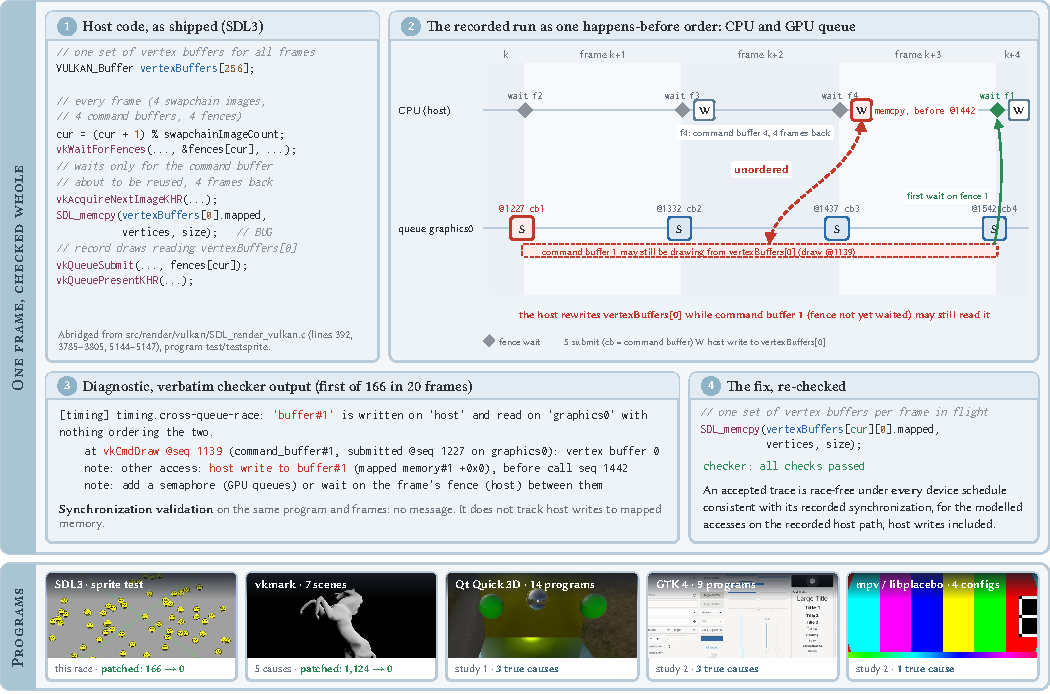
\includegraphics[width=\textwidth]{fig1-teaser.pdf}
  \caption{\textbf{One frame, checked whole: a host-write race in SDL3 that synchronization validation does not
  see.} \circled{1}~SDL3's Vulkan renderer, unmodified (\code{test/testsprite}), runs once against a GPU-free model
  driver that records every call and traps every CPU store to mapped memory. Each frame it waits for the fence of
  the command buffer it is about to reuse, four frames back, and then copies the new vertices into
  \code{vertexBuffers[0]}, of which there is one set for all frames. \circled{2}~\sys orders the recorded run as one
  happens-before relation over the CPU and the GPU queue. The store before call @1442 is ordered after the fence
  wait for command buffer~4 only; command buffer~1, whose draw @1139 reads the same buffer, is waited for only in the
  next frame, so the store and the draw are unordered. \circled{3}~The checker's verbatim diagnostic (the first of
  166 in 20 frames). Synchronization validation, run on the same program and frames on lavapipe, reports nothing: it
  does not track host writes to mapped memory. \circled{4}~With one set of vertex buffers per frame in flight the
  checker reports nothing, and Corollary~\ref{cor:sched} gives race freedom under every device schedule consistent
  with the recorded synchronization, for the modelled accesses on the recorded host path. Diagnostic from the
  checker frozen for the studies of \S\ref{sec:eval-fresh}, unchanged in the release; bug SDL-1 of
  Table~\ref{tab:bugs}; sequence numbers are from the recorded trace.}
  \label{fig:teaser}
\end{teaserfigure}

\maketitle
\hypersetup{pdfauthor={},pdfcreator={},pdfsubject={},pdfkeywords={},pdftitle={COVENANT: Schedule-Independent Verification of Vulkan Frame Synchronization}}

%% ===================================================================
\section{Introduction}
\label{sec:intro}

A graphics frame is a concurrent program. The CPU records command buffers and writes mapped memory. One or more GPU
queues execute the commands. A presentation engine reads finished images on its own clock, and the next frame starts
before the previous one has finished. Vulkan, Direct3D~12 and Metal leave the ordering of all this to the
application, which must express it through barriers, semaphores, fences and image layouts.

Mistakes in this ordering rarely fail loudly. A vertex buffer rewritten while the GPU may still read it
(Figure~\ref{fig:teaser}), a semaphore reused one frame too early, or a swapchain image acquired once too often all
pass most test runs; the last is the likely cause of a public sample freezing in about 3 of 100 runs
(\S\ref{sec:motivation}). Each of these bugs spans frames, queues or the presentation engine.

\paragraph{What existing checks cover}
Khronos synchronization validation~\cite{lunarg2021syncval} (``syncval'') is the standard tool. It runs inside the
Vulkan loader and reports potential hazards implied by the synchronization the application declares, including
hazards across command buffers, queues and swapchain operations, not only the hazards that manifest in the observed
schedule. It does not need a GPU either: on the Khronos mock driver it analyses submitted commands without executing
them, and we use it that way (\S\ref{sec:eval-wholeframe}). It does not track host accesses to mapped
memory~\cite{lunarg2021syncval}. Static GPU
verifiers~\cite{betts2012gpuverify,cogumbreiro2021faial,martinez2026kuiper,bansal2026prism} reason inside one kernel.
Render graphs~\cite{odonnell2017framegraph,amd2022rps} derive barriers at run time from declared accesses.
\rcgp~\cite{sivaram2026rcgp} makes structural misuse a compile-time error for programs written in its embedded
language, within one command recording.

\paragraph{What \sys adds}
None of \sys's ingredients is individually new: vector clocks, FastTrack-style epochs, GPU-free capture and
whole-frame reasoning all exist. What we contribute is their integration into one \emph{specified},
schedule-independent analysis of a captured Vulkan frame, and the evidence that this integration finds bugs and can
be trusted. Concretely, one analysis covers:
\begin{itemize}
\item \textbf{host memory:} CPU stores to mapped memory are captured by page protection and ordered with device
  work, including stores that leave a value unchanged (\S\ref{sec:capture}); eight of the real bugs we report are
  host-write races, a class that validation does not track;
\item \textbf{presentation and overlapping frames:} one presentation queue per swapchain image, acquire and present
  as operations on it, and every frame in flight in one order (\S\ref{sec:model});
\item \textbf{actionable diagnostics:} each report names the scope test that failed, and reports are grouped by site
  and by a repair that was re-checked on the whole frame (\S\ref{sec:algo});
\item \textbf{checked transformations:} the same decision procedure licenses barrier removal on the recorded
  execution (\S\ref{sec:elide});
\item \textbf{a soundness theorem with a full proof} that connects the implemented algorithm, as pseudocode, to a
  transcription of the specification, with a stated trusted computing base and a domain that the checker reports for
  every run (\S\ref{sec:model}, Appendix~\ref{app:proofs}).
\end{itemize}

\paragraph{Scope}
The guarantee is about the recorded host path, in the verified configuration (spec-strict layout transitions,
conservative host capture), under premises we state (\S\ref{sec:premises}). Each run's report says whether the run is
in the guarantee's domain: checking completed, no unmodelled command with a memory effect, and no host write whose
ordering relies on the host-domain premise (\S\ref{sec:eligible}). Swapchain recreation, resizes and error paths that
the run did not take are not covered, and neither are accesses outside the model (\S\ref{sec:cover}).
Semantic conventions such as color encoding or units are outside the synchronization guarantee.

\paragraph{Contributions}
\begin{enumerate}
\item \textbf{A semantics of Vulkan host orchestration and a proved checker} (\S\ref{sec:model}--\S\ref{sec:algo}).
  Soundness of the pairwise algorithm (Theorem~\ref{thm:sound}) and of the fast epoch mode
  (Lemma~\ref{lem:fast}), with full proofs, including framebuffer-local dependencies, the host-write domain
  operation and the descriptor-index refinement; conditional precision on region-uniform traces
  (Proposition~\ref{thm:complete}); and a window theorem that is conditional on periodic continuation
  (Theorem~\ref{thm:window}).
\item \textbf{A conservative capture of host writes} by page protection, with a conservativity argument and its
  measured precision cost (\S\ref{sec:capture}, \S\ref{sec:eval-fresh}).
\item \textbf{Differential validation against synchronization validation} (\S\ref{sec:eval-sem}): 750 barrier
  mutants, 13 ray-tracing and mesh-shading programs and 1,251 generated whole-frame programs with semaphores,
  swapchains, frames in flight and a second queue family, re-run with the released checker.
\item \textbf{\bench and blind evaluation} (\S\ref{sec:eval-bench}--\S\ref{sec:eval-real}): 166 real application
  bugs from 105 projects; six blind rounds with frozen checkers; two pre-registered studies of the proved
  configuration on previously unchecked programs from eight code bases, with every report group triaged by written rules and compared
  with validation; 54 bugs we judge real in public code. For 9 of them we patched the source, rebuilt and re-checked
  (11 source-patch cases); 15 programs become clean.
\end{enumerate}
Section~\ref{sec:motivation} gives motivating examples, \S\ref{sec:overview} an overview, \S\ref{sec:model} the
semantics and theorems, \S\ref{sec:algo} the algorithm, \S\ref{sec:impl} the implementation and capture,
\S\ref{sec:eval} the evaluation, \S\ref{sec:elide} the barrier application and \S\ref{sec:limits} the limitations
in one place. A supplement holds the capture and \code{UNDEFINED} design notes, the checker snapshots used by each
study, the per-engine triage, the bug dossier summary and the full results tables. The code, the model driver, the
tests and the scripts of every experiment are released with the paper.

%% ===================================================================
\section{Motivating Examples}
\label{sec:motivation}

\subsection{What a Vulkan frame must get right}
A Vulkan queue does not execute commands in submission order. Two commands are ordered only by an
\emph{execution dependency}, or by a chain of them. The earlier command must be in the first synchronization scope
(the source stages, expanded to logically earlier stages). The later command must be in the second scope (the
destination stages, expanded to logically later stages).
A write is visible to a later access only if the dependency also makes it available and visible. Availability
requires the write to be in the first \emph{access} scope, and visibility requires the later access to be in the
second. Access scopes contain only the stages named explicitly.
A layout transition is itself a write, and every earlier write must be made available before it executes, even when
the old layout is \code{UNDEFINED}. Semaphores order work between queues, fences order the host after the
device, and a semaphore wait blocks only the stages in its wait mask.
The presentation engine reads swapchain images concurrently with rendering. At most
$n_{\mathit{images}} - n_{\mathit{minImages}} + 1$ images may be held at once.
Shader-level memory models~\cite{tong2024gpuconsistency} formalize what happens inside the GPU. Our concern is the
command-level orchestration around it.

\subsection{Three bugs that span the frame}
\paragraph{A semaphore reused across frames}
\bench case 30 is a typical instance. Its render-finished semaphores are indexed by frame in flight rather than
by swapchain image. The fence the host waits on proves only that the earlier \emph{submission} has finished, not that
the \emph{present} that waits on its semaphore has consumed it, so the next signal of that semaphore may be made while
the semaphore is still signaled. No single command buffer contains the bug: it lives between the queue, the host's
fence wait and the presentation engine of one swapchain image, two frames apart.

\paragraph{Host writes racing the GPU}
In the public Sascha Willems Vulkan samples, the per-frame uniform-buffer descriptors of one sample all point at
buffer~0, while the host rewrites the buffers after waiting on only one frame's fence (SW-T1, \S\ref{sec:eval-bugs}).
The GPU may still read the buffer the CPU is writing. \sys reports a cross-queue race between the host and the
graphics queue:
\begin{lstlisting}[style=diag]
[timing] timing.cross-queue-race: 'buffer#3' is written on 'host' and read on 'graphics0' with nothing
  ordering the two. at vkCmdDrawIndexed @seq 350 (...): set 0 binding 0
    note: other access: host write to buffer#3 (mapped memory#4 +0x0), before call seq 607
\end{lstlisting}
Synchronization validation does not track host writes to mapped memory, so it cannot observe this class of race.
Several such stores write the bytes that are already there; a capture that compares memory snapshots does not see
them at all (\S\ref{sec:capture}).

\paragraph{A swapchain image acquired once too often}
In about 3 of 100 runs on a consumer GPU, one public sample of \rcgp~\cite{sivaram2026rcgp} froze inside
\code{vkAcquireNextImageKHR}. Its runtime treats a suboptimal acquire as a failed one, so the acquired image is
never presented and the swapchain is never rebuilt; the program can then hold more images than the surface allows,
and it waits with an infinite timeout. \sys reports the pattern from one trace of a distilled reproduction, recorded
on a machine with no GPU:
\begin{lstlisting}[style=diag]
[timing] timing.swapchain-overacquire: this acquire would hold 3 images of 'swapchain' at once,
  but only 2 may be held (3 images, minimum 2); it can block forever.
    at vkAcquireNextImageKHR @seq 115 (swapchain[2])
\end{lstlisting}
This is not independent evidence for \sys: the rule was written after we saw the freeze. Like the semaphore reuse
above, it is a protocol check, justified by a valid-usage rule rather than by the race theorem (\S\ref{sec:protocol}).

\subsection{What existing tools see}
\label{sec:rcgp}
Synchronization validation reasons from the declared synchronization of the command stream that the application
submits, on a real device or the mock driver; it does not see host writes, and its verdicts depend on the device and
on its configuration (\S\ref{sec:eval-real}). Render graphs prevent the barrier bugs they own, but not those in code
around them or in their own barrier derivation (VUK-1, \S\ref{sec:eval-bugs}). \rcgp~\cite{sivaram2026rcgp} is a
C++26 embedded language whose resource contracts, typed modules and combinators make programs that misuse its
abstractions fail to compile, for every execution. By design its guarantees are scoped (Table~\ref{tab:scope}):
programs are written in its language, effects cover one recording, and swapchain acquire and present, frames in
flight and multiple queues are outside its effect algebra. \sys starts at these boundaries and gives the weaker,
executed-path guarantee for existing code. The two are complementary (\S\ref{sec:eval-rcgp}).

\begin{table}[t]
\caption{Scope of \rcgp and \sys. The \rcgp column is from its paper, compile-only ports and its source.}
\label{tab:scope}
\small
\resizebox{\columnwidth}{!}{%
\begin{tabular}{@{}lll@{}}
\toprule
Property & \rcgp & \sys \\
\midrule
Input program & its C++26 eDSL & unmodified Slang/GLSL + C++ \\
Barriers & render-to-sample: inserted & stage/access checked (Thm.~\ref{thm:sound}) \\
Guarantee & every execution & executed host path \\
Multiple queues, ownership & no & yes \\
Frames in flight, swapchain & no & yes \\
Host writes to mapped memory & no & yes \\
When it runs & C++ compile time & after one GPU-free run \\
\bottomrule
\end{tabular}}
\end{table}

%% ===================================================================
\section{Overview}
\label{sec:overview}

\begin{figure*}[t]
  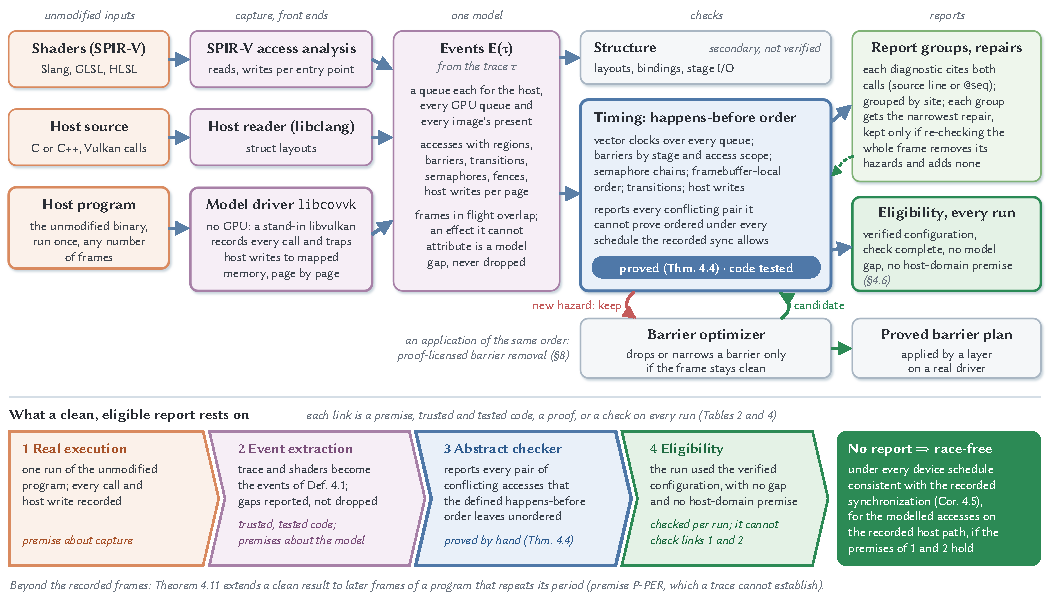
\includegraphics[width=\textwidth]{fig-overview.pdf}
  \caption{\textbf{Overview.} The unmodified host program runs once on the model driver, which records every call and
  traps host writes to mapped memory by page; shaders and host source add per-entry-point accesses and layouts. The
  timing check builds one happens-before order over the CPU, every GPU queue and the present of each swapchain image,
  across frames in flight. In the verified configuration it is proved sound for the recorded host path under the
  premises of \S\ref{sec:premises}. It covers graphics, compute, mesh-shading and ray-tracing work, and reports any
  command it does not model. Secondary structure checks share the trace. Raw diagnostics are grouped by site, and each
  group gets the narrowest barrier or mask repair, kept only if re-checking the whole frame removes the group's
  hazards and adds none. Barrier removal is an application of the same order (\S\ref{sec:elide}).}
  \label{fig:overview}
\end{figure*}

Figure~\ref{fig:overview} shows the pipeline. It has three inputs: shaders in Slang, GLSL or HLSL, compiled to SPIR-V
with debug information so that diagnostics point at source; the host source, read with libclang for struct layouts;
and the host binary, which runs unmodified against \code{libcovvk}. This stand-in \code{libvulkan} returns fake handles
and records a trace of every call (\S\ref{sec:impl}). From the trace, \sys builds an event structure over the host,
every device queue and one presentation engine per swapchain image (\S\ref{sec:model}), computes its happens-before
order and reports every conflicting pair it cannot prove ordered (\S\ref{sec:algo}).

%% =====================================================================
%% formal.tex -- Sections 4 (Formal Semantics) and 5 (Verification Algorithm).
%% The algorithm of Figure fig:alg is transcribed from covenant/timing.py of the release.
%% =====================================================================
\providecommand{\Sc}[1]{\mathit{Sc}_{#1}}
\providecommand{\ASc}[2]{\mathit{ASc}_{#1}^{#2}}
\providecommand{\ESs}{\mathit{ES}^{\mathrm{src}}}
\providecommand{\ESd}{\mathit{ES}^{\mathrm{dst}}}
\providecommand{\AS}{\mathit{AS}}
\providecommand{\chainto}{\rightsquigarrow}
\providecommand{\mspecl}[1]{\ensuremath{\Rightarrow_{m}^{#1}}}
\providecommand{\ordl}[1]{\mathit{ord}_{#1}}
\providecommand{\Hpw}{\ensuremath{\Haz_C^{\mathit{pw}}}}
\providecommand{\Hep}{\ensuremath{\Haz_C^{\mathit{ep}}}}
\providecommand{\Hspec}{\ensuremath{\Haz_{\mathit{spec}}}}
\providecommand{\kw}[1]{\textbf{#1}}
\providecommand{\pc}[1]{\textsc{#1}}
\providecommand{\posof}{\pi}
\providecommand{\Hstrict}{\ensuremath{\Haz_{\mathit{spec}}^{\mathit{dom}}}}

%% ===================================================================
\section{Formal Semantics of the Recorded Frame}
\label{sec:model}

The guarantee of \sys is a chain of steps, from a run of the host program to a statement about that run
(Table~\ref{tab:chain}). Each step is of one of three kinds: a definition or theorem that we prove
(Appendix~\ref{app:proofs}), a named premise about capture or modelling (\S\ref{sec:premises}), or trusted code
that we test but do not prove (\S\ref{sec:tcb}). We keep the three apart.

\begin{table}[t]
\caption{From captured execution to stated guarantee. ``Proved'' means proved in Appendix~\ref{app:proofs} for the
algorithm of Figure~\ref{fig:alg}, relative to our transcription of the specification
(Definitions~\ref{def:events}--\ref{def:spec}). The transcription follows the Vulkan specification at Vulkan-Docs
tag \code{v1.4.365}, the revision of the headers our model driver and validation baseline use.}
\label{tab:chain}
\small
\begin{tabular}{@{}p{0.30\columnwidth}p{0.30\columnwidth}p{0.32\columnwidth}@{}}
\toprule
Step & Bridge & Kind \\
\midrule
run $\to$ trace $\tau$ & A1, A2-H; scope A3 & premise about capture \\
$\tau \to$ events $E(\tau)$ & A2, A-HOST, A-RT/EV/DS & premise about the model \\
$E(\tau) \to \Hspec(\tau)$ & Def.~\ref{def:events}--\ref{def:spec} & definition (our transcription) \\
algorithm $\to \Hspec$ & Thm.~\ref{thm:sound}, Lem.~\ref{lem:fast} & proved, under W1 (and W2 for Lem.~\ref{lem:fast}) \\
source code $\to$ algorithm & \S\ref{sec:tcb} & trusted, tested \\
no report $\to$ run is race-free & Cor.~\ref{cor:sched} & proved from the rows above \\
no premise warning $\to$ host domain & Prop.~\ref{prop:hostdom} & proved; removes the device-to-host part of A-HOST \\
recorded frames $\to$ later frames & Thm.~\ref{thm:window} & proved, conditional on P-PER, which the trace cannot establish \\
\bottomrule
\end{tabular}
\end{table}

\subsection{Events and synchronization}
\label{sec:events}

\begin{definition}[Trace, queues and events]\label{def:events}
A trace $\tau$ is the sequence of Vulkan calls of one run, in host order. From it \sys builds a set of queues
$Q = \{\mathit{host}\} \cup Q_{\mathit{dev}} \cup \{\mathit{present}{:}i\}_i$, with one presentation queue per
swapchain image, and for each queue $q$ a sequence of operations, appended in host order: the $k$-th operation of $q$
is at position $(q,k)$, and $\mathit{call}(o)$ is the host call that appended $o$. An operation is an access, a
barrier struct, a signal $\mathsf{Sig}(x,S)$ or a wait $\mathsf{Wait}(x,W)$ of a name $x$, or an event set/reset
marker. $S$ and $W$ are stage masks or $\top$ (all stages). A queue submission is $\mathsf{Sig}(\mathit{submit}_c)$ on
the host followed by $\mathsf{Wait}(\mathit{submit}_c,\top)$ at the head of the batch on its queue. A fence or idle
wait is a signal on a device queue and a $\top$ wait on the host. Swapchain acquire and present are encoded on the
presentation queues as in \S\ref{sec:impl}. A queue's operations after a wait whose name is never signalled are
dropped.

The events $E(\tau)$ are the accesses and the layout transitions; a transition $t_B$ sits at the position of its
barrier struct $B$. An event $a$ has a queue $q(a)$, a position $p(a)$, a resource $r(a)$ and a region
$R(a)$: a set of elements, which are the bytes of a buffer, or the aspect $\times$ layer slots of one mip level of an
image. It also has a kind $k(a) \in \{\mathsf{R},\mathsf{W}\}$ (transitions are $\mathsf{W}$), a stage $s(a)$ (a
pipeline stage, $\bot$ if unknown, or the pseudo-stage $\mathsf{LT}$ for a transition), an access flag $f(a)$ ($\bot$ if
unknown), and four exemption tags: its command, its render-pass scope, its subpass instance with a load/store
marker, and its atomic mode. A transition is \emph{explicit} if an image memory barrier performs it and
\emph{automatic} if a render pass does. An event may carry a \emph{position token} $\posof(a)$
(\S\ref{sec:fblocal}); $\posof(a) = \bot$ otherwise. The frames of $\tau$ are the segments of the host's call sequence that end at each
\code{vkQueuePresentKHR}; $\mathit{fr}(o)$ is the frame that contains $\mathit{call}(o)$.
\end{definition}

\paragraph{Scopes}
For a stage mask $M$, $\ESs(M)$ and $\ESd(M)$ are its source and destination \emph{execution} stage sets. They add to
each named stage the logically earlier (source) or later (destination) stages of every synchronization pipeline
that contains it, as listed in the Vulkan registry. \code{ALL\_COMMANDS}, \code{BOTTOM\_OF\_PIPE} (source) and
\code{TOP\_OF\_PIPE} (destination) give $\top$; \code{TOP\_OF\_PIPE} (source) and \code{BOTTOM\_OF\_PIPE}
(destination) give $\emptyset$. \code{ALL\_GRAPHICS} gives the graphics and mesh stages, \code{TRANSFER} also gives
\code{COPY}, \code{BLIT}, \code{CLEAR} and \code{RESOLVE}, and the acceleration-structure build stage also gives the
copy stage. $\AS(M)$, the \emph{access} stage set, applies only these group expansions; it adds no earlier or later
stages. $\top$ contains every stage except $\mathsf{LT}$, which is in a set only if it is named, and $\bot$ is in a set
only if the set is $\top$. The two fragment-test stages are interchangeable in access sets (decision M1, as in
validation). $f \in_k A$ is access-mask membership for an access of kind $k$; \code{MEMORY\_READ} and
\code{MEMORY\_WRITE} contain every read or write, including one whose flag is $\bot$, which no other mask contains,
and \code{SHADER\_READ} does not contain \code{UNIFORM\_READ}.

\begin{definition}[Dependencies, chains, ordering and races]\label{def:spec}
A \emph{dependency} $D$ is a barrier struct $B=(S_1,A_1,S_2,A_2,r_B,R_B)$, where $r_B = \ast$ for a global
barrier; a signal; or a wait. Each $D$ has a position $p(D)$ on a queue $q(D)$. A barrier struct also has a call
identity, and an event wait has a cut $c_B$: the position of the latest set of its event before it, or $-\infty$ if
there is none or a reset followed it. Each dependency has a first and a second stage set: $\ESs(S_1)$ and $\ESd(S_2)$
for a barrier, $\ESs(S)$ for a signal and $\ESd(W)$ for a wait (empty on the side that does not apply). Host signals,
host waits and submission waits have $\top$.

\emph{Locality.} A barrier struct or subpass dependency $D$ also has a locality $\lambda(D)$: $\mathsf{loc}$ when its
dependency flags hold \code{BY\_REGION}, or \code{VIEW\_LOCAL} with view offset~0; $\mathsf{nopos}$ for
\code{VIEW\_LOCAL} with a non-zero view offset; and $\mathsf{glob}$ otherwise. Signals and waits are $\mathsf{glob}$.
$F$ is the set of framebuffer-space stages (fragment shader, early and late fragment tests, color attachment output).
An event $a$ is \emph{located} if $s(a) \in F \cup \{\bot, \mathsf{LT}\}$, that is, if it may be a framebuffer-space
operation.

\emph{Synchronization scopes.} An event $a$ with $q(a) = q(D)$ is in $\Sc{1}(D)$ if $p(a) < p(D)$, $s(a)$ is in
$D$'s first stage set, $a$ is not in another struct of $D$'s call, and $p(a) < c_D$ when $D$ is an event wait. It
is in $\Sc{2}(D)$ if $p(a) > p(D)$ and $s(a)$ is in $D$'s second stage set. Transitions are the exception: $t_B$ is
in $\Sc{1}(B)$ and $\Sc{2}(B)$, in $\Sc{1}$ of a later signal with $S = \top$, and in $\Sc{2}$ of an earlier wait
with $W = \top$ or an earlier submission wait, and in no other scope. This is membership in scopes, not in stage
sets: where the ordering below tests the stage of $t_B$ against a dependency whose scope this rule puts $t_B$ in,
the test holds, and for the link classes $t_B$ counts as framebuffer-space ($\mathsf{G}$ and $\mathsf{L}$ links
hold it, $\mathsf{N}$ links do not). No API stage mask contains $\mathsf{LT}$, so two dependencies never chain
through a transition (rule R-LT). So a write in $B$'s first access scope is ordered before $t_B$ through the link
$(B,\mathsf{G})$, and $t_B$ before an access in $B$'s second access scope.

\emph{Access scopes,} for an element $\ell$: $a \in \ASc{1}{\ell}(D)$ if $a \in \Sc{1}(D)$ and, when $D$ is a barrier
struct, $s(a) \in \AS(S_1)$, $f(a) \in_{k(a)} A_1$, and $r_B = \ast$ or ($r_B = r(a)$ and $\ell \in R_B$).
$\ASc{2}{\ell}(D)$ is defined in the same way from $S_2$ and $A_2$. A signal's access scopes are its whole
synchronization scopes, and so are a wait's. A transition is in both access scopes of its own barrier.

\emph{Links.} A \emph{link} $(D,c)$ is a dependency with a class $c \in \{\mathsf{G},\mathsf{N},\mathsf{L}\}$ that
restricts its second stage set: to all of it ($\mathsf{G}$), to its stages outside $F$ ($\mathsf{N}$), or to its
stages in $F$ ($\mathsf{L}$). A link is \emph{entered locally} when $\lambda(D) \ne \mathsf{glob}$ and it is entered
from a located event or from an $\mathsf{L}$ link. A link entered locally has class $\mathsf{N}$ or $\mathsf{L}$
($\mathsf{L}$ only if $\lambda(D) = \mathsf{loc}$); every other link has class $\mathsf{G}$.

\emph{Chaining.} $(D,c) \chainto (D',c')$ if $D$ and $D'$ are on one queue, $p(D) < p(D')$, $D$'s second stage set
restricted by $c$ meets $D'$'s first stage set in a stage other than $\mathsf{LT}$ (or in $\mathsf{LT}$, when
$D$ and $D'$ are one struct of one call: the two halves of a split transition, \S\ref{app:elide}), they are not two
structs of one call, $p(D) < c_{D'}$ when $D'$ is an event wait, and $c'$ follows the rule above; or if $D$ is $\mathsf{Sig}(x,\cdot)$, $D'$ is $\mathsf{Wait}(x,\cdot)$
and $c = c' = \mathsf{G}$. On the host, every earlier dependency chains into every later one.

\emph{Ordering.} $a \xspec b$ if $q(a) = q(b) = \mathit{host}$ and $p(a) < p(b)$, or if there is a chain $(D_1,c_1)
\chainto \dots \chainto (D_n,c_n)$ ($n \ge 1$) with $a \in \Sc{1}(D_1)$, $c_1$ given by the rule above with $D_1$
entered from $a$, $b \in \Sc{2}(D_n)$ with $s(b)$ in $D_n$'s second stage set restricted by $c_n$, and
$\posof(a) = \posof(b) \ne \bot$ if $c_n = \mathsf{L}$. $a \mspecl{\ell} b$ holds if the same is true with $a \in
\ASc{1}{\ell}(D_1)$ and $b \in \ASc{2}{\ell}(D_n)$; host program order is also a memory order, and a host wait is
treated as one (premise A-HOST, \S\ref{sec:hostdom}). The intermediate dependencies need only chain.

\emph{Races.} $a$ and $b$ \emph{conflict} if $r(a) = r(b)$, $R(a) \cap R(b) \ne \emptyset$, one of them writes, and
they are not exempt. Five kinds of pair are exempt: (E1)~two accesses of one command; (E2)~attachment accesses of one
render-pass scope on one queue (rasterization order); (E3)~a load or store operation and an access of its subpass
instance; (E4)~two accesses on one queue with compatible atomic modes, that is, wherever the bytes they may touch
overlap, both are atomic operations whose memory scope holds every invocation of the device (\code{Device},
\code{QueueFamily} or \code{CrossDevice}), or both read (bytes are buffer locations: a block member's offset plus
the descriptor's offset; an access whose member is not known may touch the whole range); (E5)~two transitions on one queue, at least one of them explicit (rule R-LT).
A store through an index taken from an atomic is an ordinary write: the atomic need not hand out distinct indices
(\code{atomicAdd(c, 0)} gives every caller the same one).
They \emph{race at} $\ell \in R(a) \cap R(b)$ if neither $\ordl{\ell}(a,b)$ nor $\ordl{\ell}(b,a)$ holds, where
$\ordl{\ell}(x,y)$ is $x \mspecl{\ell} y$ if $k(x) = \mathsf{W}$ and $x \xspec y$ otherwise. We write $a \spec b$ when
$\ordl{\ell}(a,b)$ holds for every $\ell \in R(a) \cap R(b)$. $\Hspec(\tau)$ is the set of pairs that race at some
element.
\end{definition}

\paragraph{Rule R-LT}
Layout transitions ``performed via image memory barriers execute in their entirety in submission order, relative to
other image layout transitions submitted to the same queue, including those performed by render passes'', so a pair of
transitions on one queue of which at least one is by an image memory barrier is exempt (E5). Two automatic
transitions of render passes are outside this sentence and are checked like any other pair (the matrix of transition
pairs, with the specification text and a regression test for each cell, is in \supp{B}). The order is not
transitive: ``an application must not rely on ordering of image layout transitions to influence ordering of other
commands''. R-LT therefore adds no chain, and a write ordered before the first transition but not before the second
still races the second. This wording entered the specification in v1.4.326; earlier revisions gave transitions an
implicit dependency, so R-LT is the newer, weaker rule. The same paragraph adds that the ordering ``only applies if the
implementation performs actual read/write operations during the transition''; R-LT is consistent with it, since a
transition that performs no read or write leaves nothing for the exempt pair to race on, and R-LT never orders other
commands through a transition.

\paragraph{Framebuffer-local dependencies}
\label{sec:fblocal}
A dependency with \code{BY\_REGION} is \emph{framebuffer-local} for a pair of framebuffer-space operations: it orders
them only where their framebuffer regions overlap, and \code{VIEW\_LOCAL} adds the same restriction per view. A pair
in which either operation is in a stage outside framebuffer space is ordered as by any other dependency, and a chain
with one ordinary link is ordinary. Definition~\ref{def:spec} encodes this with the link classes: $\mathsf{N}$ carries
the ordinary part of a local dependency entered from a located event, $\mathsf{L}$ its framebuffer-space part, and any
ordinary link returns the chain to $\mathsf{G}$. An $\mathsf{L}$ ending orders only an access at the source's own
position, which the trace translation records as a token: for an attachment read or write, a load, store or resolve
operation, an automatic transition of an attachment, or a single-sample input-attachment read, $\posof(a)$ is the image
with the base mip level and base layer of the view through which it is accessed. Every other access has
$\posof(a) = \bot$: a storage, sampled or uniform access of one fragment can reach any byte, so no local dependency
orders it.

\begin{lemma}[Position tokens]\label{lem:tokens}
Let $\posof(a) = \posof(b) \ne \bot$. Then every texel that $a$ and $b$ both access is accessed by each of them at the
same framebuffer coordinate and view.
\end{lemma}
\begin{proof}
A framebuffer-space operation with a token accesses, at framebuffer coordinate $(x,y)$ of view $v$, the texel
$(x,y)$ of layer $\mathit{base}+v$ of mip $\mathit{base}$ of its image, and no other texel; a single-sample input
attachment read is restricted to its own pixel by the specification. Two operations whose views have the same image,
base mip and base layer therefore map each common texel to the same coordinate and view.
\end{proof}

So an $\mathsf{L}$ chain from $a$ orders $b$ at every common texel, and treating \code{nopos} links as $\mathsf{N}$
only, and tokenless accesses as unordered by $\mathsf{L}$ links, can only add races. Traces recorded without subpass
dependency flags are read with every explicit subpass dependency local, the weaker reading. Theorem~\ref{thm:sound}
and Lemma~\ref{lem:fast} are proved for this definition (Appendix~\ref{app:sound}), and the executable reference
implements it.

\paragraph{The verified configuration}
Definition~\ref{def:spec} follows the specification on layout transitions from \code{UNDEFINED}: a write before such a
transition must be made available to it ($\ordl{\ell}$ uses $\mspecl{\ell}$ when the earlier access writes), although the
transition discards the contents. The specification requires that all memory writes be made available before a
layout transition executes, and \code{UNDEFINED} only permits the old contents to be discarded. The \emph{verified
configuration} is \sys's default: spec-strict transitions, conservative host capture (\S\ref{sec:capture}) and the
weaker reading of unrecorded subpass flags. Two opt-in switches leave it, a heuristic that accepts an execution
dependency before a transition from \code{UNDEFINED} (relaxation R1) and byte-difference host capture; each report
records its configuration, and every theorem in this paper is stated for the verified one.

%% ===================================================================
\subsection{Premises}
\label{sec:premises}

Table~\ref{tab:assume} lists the premises. They are of three kinds, plus the periodicity premises of
\S\ref{sec:window}. \emph{Capture} premises (A1, A2-H) relate the run
to the trace, and A3 states the scope. \emph{Model} premises (A2, A-HOST and the rows for ray tracing, events and
dynamic state) relate the trace to the events. \emph{Well-formedness} premises (W1, W2) hold by construction of the
trace translation. The checker's own correctness is not a premise. Section~\ref{sec:tcb} states which code is trusted and how it is
tested.

\begin{table}[tp]
\caption{Premises of the theorems, and their status. TLAS/BLAS: top-/bottom-level acceleration structure; SBT:
shader binding table; BDA: buffer device address.}
\label{tab:assume}
\footnotesize
\begin{tabular}{@{}p{0.27\columnwidth}p{0.68\columnwidth}@{}}
\toprule
Premise & Status \\
\midrule
\multicolumn{2}{@{}l}{\emph{Capture}} \\
A1 trace faithfulness & by construction of the recording driver: every call of the run with its arguments, in one
host order. A command the model does not interpret is reported (\code{timing.unmodelled-command}); no claim is made for it \\
A2-H conservative host capture & page protection: a page written between two calls is charged to every binding it
overlaps, at that call boundary (\S\ref{sec:capture}). The opt-in byte-difference capture is outside A2-H \\
A3 one host path (scope) & only the recorded path and one interleaving of host threads \\
\midrule
\multicolumn{2}{@{}l}{\emph{Model}} \\
A2 device accesses over-approximated & an event per access of a recorded command, with its stage and flag (or $\bot$)
and a region that contains it; exemption tags never claimed falsely. Byte intervals; aspect $\times$ layer per mip;
static binding use; every written element of a bound descriptor array, except under a holding index guard
(Lemma~\ref{lem:guard}). Aliasing of distinct resources is not modelled \\
A-HOST host-domain operations & host-to-device: a submission makes earlier host writes available and visible to the
device. This holds for host-coherent memory, the only host-visible memory the model driver offers, so it holds for
the recorded run; for non-coherent memory on another device it needs the application's
\code{vkFlushMappedMemoryRanges}. Device-to-host: a host wait (fence, timeline value, query with \code{WAIT}, idle)
orders the waited scope before later host events (specified), and Definition~\ref{def:spec} also treats it as a memory
order, which the specification does not grant. \sys reports every pair that relies on the latter as a premise warning;
with none reported, A-HOST is used only for host-to-device (Proposition~\ref{prop:hostdom}). Host reads are not events,
so no claim on host readback \\
A-RT1 TLAS references & read at submission from host-visible instance buffers; if unresolvable, every live BLAS \\
A-RT2 device addresses & resolved at record time against live buffers; an unmatched address is reported \\
A-RT3 shader BDA accesses & not tracked; the pipeline is listed as ``untracked'' \\
A-RT4 query results & not memory (AS properties, compacted sizes, timestamps) \\
A-RT5 \code{vkCmdTraceRays}\-\code{Indirect2KHR} & SBT in GPU memory, unknown; reported \\
A-RT6 host AS builds/copies & a host write of the destination; inputs not tracked \\
A-EV1 events & a wait is a barrier whose first scope is cut at the latest set of the event on its queue; a host
\code{vkSetEvent} orders nothing on the device (reported) \\
A-DS1 dynamic state & whitelisted state folded into the over-approximation (all bound vertex buffers read, all color
attachments written) \\
\midrule
\multicolumn{2}{@{}l}{\emph{Well-formedness} (by construction of the trace translation)} \\
W1 unique signals & each name is signalled at most once (numbered binary instances, timeline values, fence
generations) \\
W2 contiguity & the accesses of one command lie on one queue with nothing between them; no wait, signal or access of
another scope (instance) lies between two accesses of one render-pass scope (subpass instance); the structs of one
barrier call are consecutive (Lemma~\ref{lem:fast} only) \\
\midrule
P-MONO, P-WSI, P-PER & Theorem~\ref{thm:window} only (\S\ref{sec:window}); the first two and periodicity inside
$\tau$ can be checked on $\tau$, continuation beyond it cannot \\
\bottomrule
\end{tabular}
\end{table}

%% ===================================================================
\subsection{Soundness}

Let $\Hpw(\tau)$ be the set of pairs that the pairwise mode of Figure~\ref{fig:alg} reports, and $\Hep(\tau)$ the set
that the epoch mode reports.

\begin{theorem}[Soundness of the checking algorithm]\label{thm:sound}
Let $\tau$ satisfy W1, and run the algorithm of Figure~\ref{fig:alg} in the verified configuration.
If \pc{Ordered}$(a,b)$ returns \emph{ok} for conflicting events $a, b$, then $a \spec b$. Hence
$\Hspec(\tau) \subseteq \Hpw(\tau)$.
\end{theorem}

The proof (Appendix~\ref{app:sound}) follows the algorithm's own structure, in five lemmas. (i)~The order in which the
algorithm processes operations extends program order and the pairing of signals with waits. (ii)~The barrier chain
state of an event reaches exactly the links, with their classes, that a chain of Definition~\ref{def:spec} reaches
from it; in memory mode it reaches only links whose first dependency covers the whole event region. (iii)~A same-queue answer of
\emph{ok} exhibits such a chain. (iv)~An accepted relay entry of a wait record (an entry at or after $p(e)$ that passes its stage filter)
means that a chain leads from $e$ into that wait; this lemma needs W1. (v)~Each way in which a wait is accepted puts
the later event in a scope of a chain that starts at that wait. Finally, the pairwise mode presents every
earlier conflicting event as a candidate. A race is therefore never answered \emph{ok}, and it is reported unless it
is exempt, and exempt pairs are not races.

\begin{corollary}[What an accepted trace guarantees]\label{cor:sched}
Assume also A1, A2, A2-H, A-HOST and the modelling rows of Table~\ref{tab:assume}. If $\Hspec(\tau) = \emptyset$
(in particular, if the pairwise mode reports nothing, or if the epoch mode reports nothing under the premises of
Lemma~\ref{lem:fast}), then on the recorded host path every two conflicting memory accesses that the model covers are
ordered as Definition~\ref{def:spec} requires. Hence no device schedule consistent with $\tau$'s synchronization lets
them race. If, moreover, no premise warning is reported, this holds with host waits given only their specified
execution dependency (Proposition~\ref{prop:hostdom}).
\end{corollary}

The bridge from the run to $E(\tau)$ is an abstraction lemma (Appendix~\ref{app:abstraction}). A2 and A2-H give each
covered access $\alpha$ of the run a representative event $a$ whose scopes are subsets of $\alpha$'s. An ordering
of the representatives therefore implies the same ordering of the accesses, and every race of covered accesses is a
race of their representatives.

\subsection{Host-domain operations}
\label{sec:hostdom}
A device write is visible to a later host write of the same memory only after a \emph{domain operation}: a memory
dependency whose destination access mask holds \code{HOST\_READ} or \code{HOST\_WRITE}. A fence or a host wait alone
gives an execution dependency; the specification states that it does not make device results visible to the host.
Definition~\ref{def:spec} treats a host wait as a memory order, so on its own it would accept a device write followed,
after a fence wait, by a host write with no such barrier. We therefore separate that case.

\begin{definition}[Host-domain ordering]\label{def:hostdom}
A device write $e$ is \emph{host-domain ordered} before a host write $u$ if there is a barrier struct $B$ with $e
\mspecl{\ell} B$ for every $\ell \in R(e) \cap R(u)$ (a chain from $e$ whose last link is $B$), $\mathsf{HOST}$ in $B$'s
second stage and access stage sets, \code{HOST\_READ}, \code{HOST\_WRITE} or \code{MEMORY\_*} in its second access
mask, and a chain from $B$ whose last link holds $u$ in its second scope. $\Hstrict(\tau)$ is $\Hspec(\tau)$ plus every pair of a device write and a later host write
that conflict and are not host-domain ordered.
\end{definition}

\sys checks this for every pair it accepts in which a device write precedes a host write: it looks for such a $B$ on
the write's queue, reached by the write's memory chain and recorded before the latest position of that queue that a
host wait holds through signals of every stage. When there is none, it reports the pair as a premise warning
(\code{timing.premise-host-domain}). The test is conservative: a domain operation on another queue is not credited.

\begin{proposition}[Host domain]\label{prop:hostdom}
Under the premises of Theorem~\ref{thm:sound}, if the pairwise mode, or the epoch mode under W2, reports no error and
no premise warning, then $\Hstrict(\tau) = \emptyset$.
\end{proposition}

The proof (Appendix~\ref{app:hostdom}) shows that an accepted pair without a warning has the barrier the definition
asks for, and that in epoch mode a write that stands in for a dropped device write carries the domain operation over to
it, as in Lemma~\ref{lem:fast}. In the opposite direction no premise is left for the recorded run: the model driver
offers only host-coherent host-visible memory, where a submission performs the host-to-device domain operation. On a
device whose application chooses non-coherent memory, the host path differs (A3) and its flushes become a premise.

\subsection{Descriptor arrays}
\label{sec:guards}
A2 charges a draw with a read of every written element of each descriptor array its shaders use statically, which is
sound but imprecise when a shader selects one element per instance. \sys narrows the read only when it can show which
elements a draw can select. An \emph{index guard} $g$ of a direct, non-indexed draw $d$ holds when: (C1) every index
into the array is a constant or a chain of at most four constant shifts and masks of one flat 32-bit integer vertex
attribute; (C2) the pipeline has only vertex and fragment stages, no dynamic vertex-input state and no instance
divisor; (C3--C4) every attribute word $d$ fetches lies in host-written pages with recorded contents, rebuilt as of
$d$'s submission; (C5) no device command writes those bytes, and no image is bound on them; (C6) no host write to them
races $d$'s vertex-input read, and none recorded after the submission is ordered before it; (C7) every decoded index is
in range; (C8) the array holds sampled images. The decoded set $I(d)$ is the image of the decoded words under the
index chain. Under a holding guard, elements outside $I(d)$ are charged only if the guard fails.

\begin{lemma}[Index guards]\label{lem:guard}
Let $g$ hold for draw $d$ in the final check. Then in every device schedule consistent with $\tau$'s synchronization,
every invocation of $d$ indexes the array only with elements of $I(d)$, so the narrowed events still represent every
access of the run (A2).
\end{lemma}

The proof (Appendix~\ref{app:guard}) has three steps: the vertex fetch reads the rebuilt bytes in every schedule,
because no device command writes them (C5), every host write to them is ordered before the draw at or before its
submission or makes the guard fail (C6), and a race with any of them would be reported by Theorem~\ref{thm:sound}; the
shader maps those bytes into $I(d)$ (C1, C2, C7); and the events dropped therefore stand for no access. The guard is
not self-supporting: C5 and C6 mention only events on the attribute bytes, which are buffer bytes, and the
happens-before order, while the events a guard removes are image reads (C8), and accesses create no dependencies. So
the set of failing guards is the same whether or not the conditional reads are present; the checker computes it by
re-running with failed guards widened until no new guard fails. Any other index source (push constants, uniforms,
storage buffers, indirect or indexed draws) keeps the full charge.

\subsection{Guarantee eligibility}
\label{sec:eligible}
Every check reports three facts separately. \emph{Checking complete}: every queue ran to its end (no wait was left
without a signal). \emph{Reporting complete}: report grouping finished within its budget; when it does not, every
diagnostic is still reported, as a site group without a repair, and the result is marked incomplete (grouping never
removes a diagnostic, so this does not affect the guarantee). \emph{Guarantee-eligible}: the verified configuration,
checking complete, no detected capture or coverage violation (an unmodelled command, an untracked mapping, a capture
warning, host writes from another thread, a pipeline whose shader code is missing or cannot be read, or that reaches
descriptor memory through a value the shader analysis cannot attribute to a descriptor), and no premise
warning. The configuration is resolved once per check, from the environment and any explicit argument, and the
same values drive the check and the reported eligibility, so a check run with an opt-in heuristic is never reported
as verified. For an eligible trace, an empty error report is an
instance of Corollary~\ref{cor:sched} and Proposition~\ref{prop:hostdom}; P2 and the model premises remain assumptions.
\S\ref{sec:eval} reports eligibility per evaluated trace.

\paragraph{What the theorem covers, and what it does not}
\label{sec:cover}
\emph{Proved:} Theorem~\ref{thm:sound} and Lemma~\ref{lem:fast} relate the algorithm to
Definitions~\ref{def:events}--\ref{def:spec}. They are proved by hand, not mechanized, and relative to our
transcription of the specification, whose fidelity the differential tests of \S\ref{sec:eval-sem} test against
synchronization validation. \emph{Assumed about capture:}
\begin{itemize}
\item \emph{trace faithfulness} (A1): the trace holds the calls of this run, in host order;
\item \emph{conservative host capture} (A2-H): for every CPU store $\sigma$ to mapped memory, the trace has a host
  write event $w$ whose region contains $\sigma$'s bytes on every resource bound there, and every event ordered
  before $w$ (after $w$) is ordered before (after) $\sigma$. Page protection gives this: the first store to a page
  after a call faults and marks the page, the driver re-protects every page at the next call, and the write is
  placed between those two calls, where the host queue has no other operation. It does not depend on whether the
  store changed a value. The byte-difference mode charges only changed bytes, and is therefore a heuristic outside
  the corollary; so is the page-straddle rule that charges a shared page only to recently bound buffers;
\item \emph{the recorded host path only} (A3): no other path or host-thread interleaving.
\end{itemize}
\emph{Assumed about the model:} over-approximated device accesses (A2), the host-domain operations (A-HOST) and the
modelling rows of Table~\ref{tab:assume}. \emph{Not covered:} host paths the run did not take, including other
driver responses such as image counts, \code{VK\_SUBOPTIMAL\_KHR} results and swapchain recreation; other
interleavings of a multithreaded host; host \emph{reads} of mapped memory; accesses through aliased memory of distinct
resources; shader device-address accesses (A-RT3), query results (A-RT4), the inputs of host acceleration-structure
builds (A-RT6) and unmodelled commands; memory ordering inside a shader; and semantic conventions. The protocol checks
of \S\ref{sec:protocol} are separate guarantees, not consequences of Theorem~\ref{thm:sound}.

%% ===================================================================
\subsection{Precision}
\label{sec:precision}

An exact access abstraction does not, by itself, make the checker exact. Exact accesses fix $E(\tau)$, but they do
not make the decision procedure exact. The algorithm decides whether a
dependency covers an access with one region test (``the barrier's region contains the whole access region''), while
Definition~\ref{def:spec} decides element by element. For example, let a write $a$ cover bytes $[0,256)$, let one
barrier call carry two buffer structs for $[0,128)$ and $[128,256)$, and let a read $b$ of $[0,256)$ follow. Every
byte is ordered, so the pair is not a race. Neither struct contains all of $R(a)$, however, so the pairwise mode
reports it. What does hold is the following.

\begin{proposition}[Conditional precision of the pairwise mode]\label{thm:complete}
Let $\tau$ satisfy the premises of Theorem~\ref{thm:sound}. Assume further that (i)~no signal has a stage mask other
than $\top$, and (ii)~$\tau$ is \emph{region-uniform}: for every barrier struct $B$ with a region on resource $r$ and
every event $a$ on $r$, either $R_B \supseteq R(a)$ or $R_B \cap R(a) = \emptyset$. Then $\Hpw(\tau) = \Hspec(\tau)$.
\end{proposition}

Condition (ii) is the missing condition, and it can be met by construction. Splitting every access at all barrier
region bounds on its resource yields a region-uniform trace $\tau^\sharp$ with the same races (the parts of one access
are disjoint, so they never conflict, and Definition~\ref{def:spec} is decided per element; Appendix~\ref{app:precision}).
The pairwise mode on $\tau^\sharp$ is exact under (i). The checker does not split, so it may report
pairs that are not races when barrier regions cut accesses (the generator setting with partial region coverage,
\S\ref{sec:eval-sem}).
Without (i), the relay of a masked signal keeps a bounded number of stage-filtered entries per queue
(Figure~\ref{fig:alg}), and dropping one only removes orderings, so the checker can be stricter there.
The proposition is exact relative to $E(\tau)$. Relative to the \emph{run}, a report can also come from the
abstraction: an over-approximated region, an unknown stage or flag (which lies only in scopes of every stage or every
access), a captured host page, or a choice of the transcription that is stricter than the specification
(\S\ref{sec:eval-wholeframe}). Exact events remove the first three, but not a region cut, which is why an exact access
abstraction alone does not make the checker exact. The epoch mode reports a subset of $\Hpw$
(Lemma~\ref{lem:modes}), so it can miss pairs, but it flags at least one event of every race (Lemma~\ref{lem:fast}).

%% ===================================================================
\subsection{Periodic executions}
\label{sec:window}

A trace covers finitely many frames. A program usually runs longer, so we ask when a finite window decides the race
freedom of every later frame. The answer is conditional, because the future is not in the trace.

\begin{definition}[Periodic continuation]\label{def:periodic}
$\tau$ is \emph{periodic after warm-up $w$ with period $p$} if there is a shift $\sigma$ from the operations of frames
$\ge w$ onto those of frames $\ge w+p$. The shift preserves queues (up to a permutation of the swapchain images),
program order, all attributes up to a renaming of resources and synchronization objects, and the pairing of waits with
signals, and it maps frame $i$ onto frame $i+p$. Its \emph{periodic continuation} $\tau^\infty$ is the unique infinite
event structure whose first frames are those of $\tau$ and on which $\sigma$ extends to all frames $\ge w$.
\end{definition}

The premises are these. \textbf{P-MONO}: every wait is paired with a signal appended earlier in host order (no
wait-before-signal). \textbf{P-WSI}: every device access to a swapchain image is recorded in a command submitted
after an acquire of that image and before its next present, and no other event touches a swapchain image.
\textbf{P-PER}: the run continues as $\tau^\infty$. The parameters are properties of $\tau^\infty$; because $\sigma$
preserves them, they can be measured on the first $w+p+D$ frames of $\tau$. $N$ is the least number such
that, before the first submission or host access of each frame $j \ge w$, the host has waited on a $\top$ signal of
every device queue that follows all that queue's operations of frames $\le j - N$. $G$ is the largest frame distance
between a device access $b$ to a swapchain image and the acquire it is held under or the present that ends it.

\begin{theorem}[Window, conditional on periodic continuation]\label{thm:window}
Let $\tau$ be periodic after $w$ with period $p$, satisfy P-MONO, P-WSI and the premises of Theorem~\ref{thm:sound},
and let $D = \max(N, G+1)$ and $M = w + p + D - 1$. Every race of $\tau^\infty$ has a translate of a witness race in
the first $M$ frames. Hence, if $\tau$ has at least $M$ frames, $\Hspec(\tau^\infty) = \emptyset$ if and only if the
first $M$ frames of $\tau$ have no race. Under P-PER, a checker-clean window therefore implies race freedom of the
whole run (Corollary~\ref{cor:sched}).
\end{theorem}

The derivation (Appendix~\ref{app:window}) uses three facts. First, by P-MONO every chain runs forward in host order,
so the ordering of two events depends only on the operations appended between them, and a prefix of $\tau^\infty$ has
the same races as $\tau^\infty$ on its events. Second, two events that are not presentation-engine events and lie $N$
or more frames apart are ordered through the host's fence or idle wait. Third, presentation-engine accesses are
\emph{not} bounded by any frame fence. A fence proves that a submission has completed, never that the present waiting
on its semaphore, or the engine's read of the image, has. They are bounded through the acquire of the same image
instead. Under P-WSI, if a device access $b$ races any presentation-engine read of its image, then it also races
either the read that ends at the acquire that $b$ is held under, or the read of the present that ends it, and both lie
within $G$ frames of $b$. $G$ is 0 when every frame acquires, renders to and presents its own image.

\paragraph{What the trace can and cannot establish}
P-MONO, P-WSI, $N$, $G$ and periodicity within $\tau$ are properties of the trace, and can be checked on it.
P-PER is a claim about host behaviour after the trace ends, which input, resizing or streaming can change, and no
finite trace establishes it. Theorem~\ref{thm:window} therefore does not by itself license applying a barrier plan to
frames that were not traced. Section~\ref{sec:elide} restricts the transformation guarantee to the recorded execution,
and makes no claim about reusing a plan beyond it. The window analysis of the checker
computes $N$ from device queues only, compares frame signatures that abstract which signal each wait consumes, and
checks $w + N + 2$ frames. That bound reaches $M$ only when $p + \max(N, G+1) \le N + 3$, for example when $p \le 3$
and $G < N$, and its $N$ ignores the presentation queues. We therefore report it as a measurement on the traces and
not as an instance of the theorem (\S\ref{sec:eval-sem}).

%% ===================================================================
\subsection{Trusted computing base}
\label{sec:tcb}

Theorem~\ref{thm:sound} and Lemma~\ref{lem:fast} are proved for the algorithm of Figure~\ref{fig:alg}, not for its
Python source. We do not assume that ``the checker implements the specification relation''. Instead we state an
explicit trusted computing base: the code whose agreement with the model we trust, and how each
part is tested (Table~\ref{tab:tcb}). Everything else (report grouping and repair synthesis, diagnostic text, the
structure checks, the window analysis, the optimizer's search) is outside it. Their errors can cost precision or
readability, but they cannot turn a race into an accepted trace, because every verdict passes through T4.

\begin{table}[t]
\caption{Trusted computing base and how each part is tested.}
\label{tab:tcb}
\small
\begin{tabular}{@{}p{0.30\columnwidth}p{0.64\columnwidth}@{}}
\toprule
Trusted code & Tested by \\
\midrule
T1 recording driver (\code{covvk.cpp}): calls, arguments, host-write pages (A1, A2-H) & the same binaries under
synchronization validation in the whole-frame (1,251 programs) and ray-tracing/mesh (13) differential tests; capture
tests \\
T2 trace translation (\code{host\_trace}, \code{ranges}, SPIR-V access analysis): events, regions, exemption tags,
W1, W2 & unit tests, including assembled SPIR-V that varies helper calls, descriptor offsets and atomic against
plain accesses; the two whole-frame differential tests; 114 \bench reproductions. The executable reference consumes
T2's events, so it does not test T2 \\
T3 stage and access algebra (pipeline tables, scope expansion) & regression unit tests; an executable reference
with independently written tables; 750 barrier mutants under validation \\
T4 checker core (run loop, \pc{Ordered}, chain state, \pc{Access}) & executable reference agreement
(\S\ref{sec:eval-sem}); property tests of $\Hspec \subseteq \Hpw$, $\Hep \subseteq \Hpw$ and criterion E on random
frames; the differential tests above \\
\bottomrule
\end{tabular}
\end{table}

%% ===================================================================
\section{Verification Algorithm}
\label{sec:algo}

Figure~\ref{fig:alg} gives the algorithm as \sys implements it. One pass processes every queue in
turn, as far as its next unsatisfied wait, until no queue can progress. Each queue has a vector clock
$\mathit{VC}[q]$~\cite{mattern1989virtual}. A signal records a copy of its queue's clock, and a wait joins the
recorded clock into its own and keeps a \emph{wait record}. A signal also records a \emph{relay}: for each queue,
the positions of that queue known to be in the signal's first scope along the whole path of semaphores that reached
it, each with the stage filter of a masked signal at its first hop. Barrier structs are appended to a per-queue list. Each
access, and each transition, is handed to \pc{Access}, which compares it with earlier events on the same resource.

\begin{figure*}[tp]
\scriptsize
\begin{minipage}[t]{0.49\textwidth}
\begin{tabbing}
\quad\=\quad\=\quad\=\quad\=\quad\=\kill
\kw{procedure} \pc{Check}$(\tau, \mathit{mode})$ \hfill \emph{Algorithm 1} \\
1\>$\mathit{VC}[q] \gets 0$; $\mathit{Bars}[q], \mathit{Waits}[q] \gets [\,]$; $\mathit{Full}[q] \gets 0$; $\mathit{RA}[q], \mathit{RF}[q] \gets \emptyset$ \quad for all $q$ \\
2\>\kw{repeat} \kw{for} $n$ \kw{in} queues \kw{while} $n$ has a next operation $o$: \\
3\>\>\kw{if} $o = \mathsf{Wait}(x,W)$: \kw{if} $x$ not yet signalled: \kw{break} \\
4\>\>\>$(c, \rho) \gets \mathit{Sig}[x]$; $E \gets \top$ \kw{if} $W{=}\top$ or $n{=}\mathit{host}$ \kw{else} $\ESd(W)$ \\
5\>\>\>\kw{if} $E \setminus \{\mathsf{LT}\} \ne \emptyset$: $\mathit{VC}[n] \gets \max(\mathit{VC}[n], c)$; push $w = (E, |\mathit{Bars}[n]|, \rho)$ onto $\mathit{Waits}[n]$ \\
6\>\>\>\>$\mathit{RA}[n] \gets \mathit{RA}[n] \sqcup \rho$; \kw{if} $E = \top$: $\mathit{RF}[n] \gets \mathit{RF}[n] \sqcup \rho$ and \\
\>\>\>\>\>$\mathit{Full}[n][m] \gets \max(\cdot, t)$ for every unfiltered $(t, \bot) \in \rho[m]$ \\
7\>\>$\mathit{VC}[n][n] \mathrel{+}= 1$; $t \gets \mathit{VC}[n][n]$ \hfill $\triangleright$ $t = p(o)$ \\
8\>\>\kw{if} $o = \mathsf{Sig}(x,S)$: $\mathit{Sig}[x] \gets (\mathit{VC}[n], \pc{Relay}(n, t, S))$ \\
9\>\>\kw{if} $o$ is a barrier struct $B$: append $(t,B)$ to $\mathit{Bars}[n]$; \kw{if} $B$ transitions: \pc{Access}$(t_B)$ \\
10\>\>\kw{if} $o$ is an access: \pc{Access}$(o)$ \\
11\>\kw{until} no queue progressed; report \code{deadlock} for blocked queues \\[3pt]
\kw{function} \pc{Relay}$(n, t, S)$ \quad $\triangleright$ per queue $m$: entries $(t_m, \varphi)$ \\
1\>$\varphi_0 \gets \bot$ \kw{if} $S{=}\top$ \kw{else} $(n, t, |\mathit{Bars}[n]|, \ESs(S))$; $\rho \gets \{n \mapsto (t, \varphi_0)\}$ \\
2\>\kw{if} $S = \top$: \kw{return} $\rho \sqcup \mathit{RA}[n]$ \hfill $\triangleright$ every wait chains into it \\
3\>\kw{if} $\ESs(S) \setminus \{\mathsf{LT}\} \ne \emptyset$: $\rho \gets \rho \sqcup \mathit{RF}[n]$ \\
4\>\kw{for} $w$ \kw{in} $\mathit{Waits}[n]$ with $w.E \ne \top$: \kw{if} $\pc{Chain}(w).X_{\mathit{tot}}$ meets $\ESs(S)$: $\rho \gets \rho \sqcup w.\rho$ \\
5\>\kw{return} $\rho$ \\[3pt]
\kw{function} \pc{Ordered}$(e, u)$ \quad $\triangleright$ $e$ processed before $u$; $m{=}q(e)$, $n{=}q(u)$ \hfill \emph{Algorithm 2} \\
1\>$\mathit{mem} \gets (k(e) = \mathsf{W})$;\ $O \gets R(e) \cap R(u)$ \hfill $\triangleright$ verified configuration$^\dagger$ \\
2\>\kw{if} $m = n = \mathit{host}$: \kw{return} ok \\
3\>\kw{if} $m = n$: $C \gets \pc{Chain}(e)$ advanced over $\mathit{Bars}[n]$ \\
4\>\>\kw{if} $u = t_B$: \kw{if} $C$ reached $B$ last, globally, or locally with $\posof(e){=}\posof(u){\ne}\bot$ \\
\>\>\>\>\kw{or} $e \in \Sc{1}(B)$ (and $e \in \ASc{1}{\ell}(B)\ \forall \ell \in O$ if $\mathit{mem}$; and, if \\
\>\>\>\>$\lambda(B) {\ne} \mathsf{glob}$ and $e$ located, $\lambda(B){=}\mathsf{loc}$ and $\posof(e){=}\posof(u){\ne}\bot$): \kw{return} ok \\
5\>\>\kw{elif} $C.\pc{Reaches}(u, \mathit{mem}, O)$: \kw{return} ok \\
6\>\>\kw{return} ok \kw{if} \pc{ViaWait}$(e,u,\mathit{mem},O)$ \kw{else} \emph{same} \\
7\>\kw{if} $\mathit{VC}[n][m] < p(e)$: \kw{return} \emph{race} \\
8\>\kw{return} ok \kw{if} \pc{ViaWait}$(e,u,\mathit{mem},O)$ \kw{else} \emph{wait} \\[3pt]
\kw{function} \pc{ViaWait}$(e,u,\mathit{mem},O)$ \\
1\>\kw{if} $\mathit{Full}[n][m] \ge p(e)$: \kw{return} true \\
2\>\kw{for} $w$ \kw{in} $\mathit{Waits}[n]$, newest first: \\
3\>\>\kw{if} no $(t, \varphi) \in w.\rho[m]$ has $t \ge p(e)$ and ($\varphi = \bot$ or $\pc{InSignal}(e, \varphi)$): \kw{continue} \\
4\>\>\kw{if} $w.E = \top$: \kw{return} true \hfill $\triangleright$ transitions included \\
5\>\>\kw{if} $u = t_B$: \kw{if} $\pc{Chain}(w).x_{\mathit{last}} = p(u)$: \kw{return} true; \kw{continue} \\
6\>\>\kw{if} $s(u) \in w.E$ \kw{or} $\pc{Chain}(w).\pc{Reaches}(u,\mathit{mem},O)$: \kw{return} true \\
7\>\kw{return} false \\[3pt]
\kw{function} \pc{InSignal}$(e, \varphi = (q, t, k, E_S))$ \quad $\triangleright$ $e$ in the first scope of a masked signal \\
1\>\kw{if} $E_S = \top$ \kw{or} ($e$ not a transition and $s(e) \in E_S$): \kw{return} true \\
2\>$C \gets$ fresh $\pc{Chain}(e)$ advanced over $\mathit{Bars}[q][0..k)$ \\
3\>\kw{return} all reached $M$ and $M^L$ sets meet $E_S$ \kw{if} $k(e){=}\mathsf{W}$ \kw{else} $C.X_{\mathit{tot}} \cup C.X^L_{\mathit{tot}}$ meets $E_S$
\end{tabbing}
\end{minipage}\hfill
\begin{minipage}[t]{0.49\textwidth}
\begin{tabbing}
\quad\=\quad\=\quad\=\quad\=\quad\=\kill
\kw{state} \pc{Chain}$(e)$: global sets $X, M$ and local sets $X^L, M^L$, each \hfill \emph{Algorithm 3} \\
\>as $(\cdot)_o$ for earlier calls and $(\cdot)_c[\cdot]$ per struct of the current call; \\
\>$X_{\mathit{tot}}, X^L_{\mathit{tot}}$; $M_{\mathit{ends}}, M^L_{\mathit{ends}}$; last reached positions; $\mathit{snap}[\cdot]$; $\posof_e$ \\
\>starts at the first barrier at or after $p(e)$ with all sets empty; \\
\>a wait record's chain starts after the wait, seeded $X_o = M_o = X_{\mathit{tot}} = w.E$ \\
\kw{procedure} \pc{Advance} over the next barrier $(t, B)$ of $q(e)$: \\
1\>\kw{if} $B$ sets (resets) event $v$: save (delete) $\mathit{snap}[v]$ of all four sets; \kw{next} \\
2\>\kw{if} $B$ starts a new call: fold $(\cdot)_c$ into $(\cdot)_o$ for all four sets \\
3\>$Y_f \gets Y_o \cup Y_c[B.\mathit{st}]$ for $Y \in \{X, M, X^L, M^L\}$; or $\mathit{snap}[v]$ if $B$ waits on $v$ \\
4\>$d_x \gets e \in \Sc{1}(B)$ (a transition only for its own $B$); $\mathit{lo} \gets d_x \wedge e$ located \\
5\>$d_m \gets d_x \wedge k(e){=}\mathsf{W} \wedge s(e) \in \AS(S_1) \wedge f(e) \in_{\mathsf{W}} A_1 \wedge (r_B{=}\ast \vee (r_B{=}r(e) \wedge R_B \supseteq R(e)))$ \\
\>\>(a transition: $d_m \gets d_x$) \\
6\>\kw{if} $\lambda(B) = \mathsf{glob}$: $g_x \gets d_x \vee (X_f \cup X^L_f)$ meets $\ESs(S_1)$; $l_x \gets$ false \\
\>\kw{else}: $g_x \gets (d_x \wedge \neg\mathit{lo}) \vee X_f$ meets $\ESs(S_1)$; $l_x \gets \mathit{lo} \vee X^L_f$ meets $\ESs(S_1)$ \\
7\>\kw{if} $g_x$: $X_c[B.\mathit{st}], X_{\mathit{tot}} \mathrel{\cup}= \ESd(S_2)$ \hfill $\triangleright$ class $\mathsf{G}$ \\
8\>\kw{if} $l_x$: $X_c[B.\mathit{st}], X_{\mathit{tot}} \mathrel{\cup}= \ESd(S_2) \setminus F$; \hfill $\triangleright$ $\mathsf{N}$ \\
\>\>\kw{if} $\lambda(B) = \mathsf{loc}$: $X^L_c[B.\mathit{st}], X^L_{\mathit{tot}} \mathrel{\cup}= \ESd(S_2) \cap F$ \hfill $\triangleright$ $\mathsf{L}$ \\
9\>the same for $g_m, l_m$ from $d_m$, $M_f$, $M^L_f$, adding $(r_B, R_B, S_2, A_2)$ to $M_{\mathit{ends}}$ \\
\>\>(restricted to stages outside $F$ for $\mathsf{N}$) or to $M^L_{\mathit{ends}}$ (stages in $F$) \\
\kw{function} \pc{Reaches}$(u, \mathit{mem}, O)$: \quad $\mathit{at} \gets \posof_e = \posof(u) \ne \bot$ \\
1\>\kw{if} $\neg\mathit{mem}$: \kw{return} $s(u) \in X_{\mathit{tot}}$ \kw{or} ($\mathit{at}$ \kw{and} $s(u) \in X^L_{\mathit{tot}}$) \\
2\>\kw{return} $\exists (r_B, R_B, \Sigma, A_2)$ in $M_{\mathit{ends}}$, or in $M^L_{\mathit{ends}}$ if $\mathit{at}$: \\
\>\>($r_B{=}\ast$ \kw{or} $r_B{=}r(u) \wedge R_B \supseteq O$) $\wedge$ $s(u) \in \Sigma \cap \AS(S_2) \wedge f(u) \in_{k(u)} A_2$ \\[3pt]
\kw{procedure} \pc{Access}$(u)$ \quad $\triangleright$ per resource: an interval map of segments \hfill \emph{Algorithm 4} \\
\>\>$\triangleright$ each segment $\varsigma$ holds $\mathit{Wr}_\varsigma$, $\mathit{Rd}_\varsigma[\kappa]$, $\mathit{Sh}_\varsigma$ \\
1\>$K \gets \mathit{Wr}_\varsigma$ (+ all $\mathit{Rd}_\varsigma$ if $k(u){=}\mathsf{W}$) for segments $\varsigma \subseteq R(u)$, \\
\>\>+ $\{e : (e,d) \in \mathit{Sh}_\varsigma \text{ live},\ d,u \text{ exempt},\ k(e){=}\mathsf{W} \vee k(u){=}\mathsf{W}\}$ \\
2\>\kw{for} each $e \in K$ once: \kw{if} $e,u$ exempt (E1--E4): $v[e] \gets$ \emph{exempt}; \kw{next} \\
3\>\>$y \gets \pc{Ordered}(e,u)$ \\
4\>\>\kw{if} $y \ne$ ok \kw{and} $(e,u)$ an E5 pair: $v[e] \gets$ \emph{lt}; $K \mathrel{+}= e.\mathit{hid}$ \\
5\>\>\kw{elif} $y \ne$ ok: report $(e,u,y)$; $v[e] \gets y$ \\
6\>\>\kw{elif} $e$ a device write, $u$ a host write, \kw{not} \pc{HostDomain}$(e,u)$: \\
\>\>\>warn $(e,u)$; $v[e] \gets$ \emph{premise} \quad \kw{else} $v[e] \gets$ ok \\
7\>\kw{if} $\mathit{mode} = \mathit{pairwise}$: add $u$ to each $\varsigma$; \kw{return} \\
8\>\kw{for} each segment $\varsigma \subseteq R(u)$: \hfill $\triangleright$ epoch mode \\
9\>\>\kw{if} $k(u) = \mathsf{W}$: \kw{for} $e \in \mathit{Wr}_\varsigma$ with ($v[e]{=}$ok and $u$ not atomic) or \pc{Supersedes}$(u,e)$, \\
\>\>\>\>and $e \in \mathit{Rd}_\varsigma$ with $v[e]{=}$ok and $u$ not atomic: \pc{Drop}$(e,u)$; add $u$ to $\mathit{Wr}_\varsigma$ \\
10\>\>\kw{else} $\kappa \gets (q,s,\text{scope},\text{instance},\text{load/store},\text{atomic},\posof)(u)$; \\
\>\>\>$\mathit{Rd}_\varsigma[\kappa] \gets [u]$, plus the newest read of another command if $u$ has one \\
\pc{Drop}$(e,u)$: remove $e$ from $\varsigma$; \kw{if} $u$ has a command, scope or instance: \\
\>\>add $(e,u)$ to $\mathit{Sh}_\varsigma$; \kw{if} $u$ is a transition: $u.\mathit{hid} \mathrel{+}= e$ \hfill $\triangleright$ R-LT \\
\pc{Supersedes}$(u,e)$: same queue, stage, flag, scope, instance, load/store \\
\>marker, atomic mode and token; both writes, neither a transition \\
\>nor in a barrier call, and not one command \\
\pc{HostDomain}$(e,u)$: $C \gets$ fresh \pc{Chain}$(e)$ over $\mathit{Bars}[q(e)]$ up to $\mathit{Full}[\mathit{host}][q(e)]$; \\
\>\kw{return} $C.\pc{Reaches}(h, \mathsf{true}, O)$ for a host access $h$ of $r(e)$ with \\
\>flag \code{HOST\_READ} or \code{HOST\_WRITE} \hfill $\triangleright$ Def.~\ref{def:hostdom}
\end{tabbing}
\end{minipage}
\caption{The checking algorithm as implemented in \sys (\code{covenant/timing.py}), verified configuration. ``Meets''
is intersection of stage sets, where $\top$ meets every set that has a stage other than $\mathsf{LT}$. A relay $\rho$
maps each queue $m$ to entries $(t, \varphi)$: the operations of $m$ at positions $\le t$ are in the first scope of
the signal along the whole path, all of them if $\varphi = \bot$, or only those that pass \pc{InSignal} for the
masked signal $\varphi$ at the first hop. $\sqcup$ merges relays, keeping per queue the largest unfiltered entry and
at most four newer filtered ones; dropping an entry only removes orderings. $\mathit{RA}[n]$ and $\mathit{RF}[n]$
merge the relays of all waits and of the full waits on $n$. A shadow entry is live while its dominator's command,
scope or instance is still current on its queue. In Algorithm~3, the global sets hold links of classes $\mathsf{G}$
and $\mathsf{N}$ and the local sets links of class $\mathsf{L}$ (Definition~\ref{def:spec}); a local link orders only
an access with the source's token $\posof_e$. \pc{InSignal} tests the union of global and local sets, since a signal
is an ordinary link. $^\dagger$Under the opt-in heuristic R1, $\mathit{mem}$ is false when $u$ is a transition from
\code{UNDEFINED}; that mode is outside the theorems.}
\label{fig:alg}
\end{figure*}

\paragraph{Invariants}
Four invariants carry the proof, and they are the reason for each data structure of Figure~\ref{fig:alg}.
\begin{enumerate}
\item \emph{Processing order is a linearization.} Operations are processed queue by queue, each wait only after its
  signal, so every chain of Definition~\ref{def:spec} runs forward in processing order (Lemma~\ref{lem:lin}). An
  earlier event is therefore always available when a later one is checked, and a queue whose clock entry for $m$ is
  below $p(e)$ has no chain from $e$ at all (Algorithm~2, line~7).
\item \emph{The chain state is exactly the reachable links.} For a source event $e$, \pc{Chain}$(e)$ walks the barriers
  after $e$ on its queue once, incrementally, and keeps the union of the second stage sets of the links it has
  reached, split by class: $X$ and $M$ hold the $\mathsf{G}$ and $\mathsf{N}$ links (orderings valid for every access
  of those stages) and $X^L$, $M^L$ the $\mathsf{L}$ links (valid only at $e$'s own framebuffer position). The structs
  of the current call are kept apart, because structs of one call never chain into one another, and an event wait
  continues only from what had been reached at its event's set. The memory sets admit a first link only if it holds
  all of $R(e)$ in its first access scope (Lemma~\ref{lem:chain}).
\item \emph{A relay entry is a chain into the signal.} An entry $(t,\varphi)$ for queue $m$ in a signal's relay
  means that every operation of $m$ up to $t$ that passes the stage filter $\varphi$ reaches the signal by a chain
  (Lemma~\ref{lem:clock}). A wait record keeps that relay, so a cross-queue question becomes a same-queue question on
  the waiting queue: does the wait's own chain reach $u$ (Algorithm~2, \pc{ViaWait})?
\item \emph{Every dropped entry has a live stand-in.} In epoch mode an entry is removed only when a later access
  orders everything it would order: a write ordered after it, a write with the same stage, flag, scope, instance,
  atomic mode and token, or a read with the same key (including the token). Where the stand-in may be exempt from a
  later access that the dropped entry is not (same command, scope or instance), the entry is kept in a shadow list
  (Lemma~\ref{lem:fast}).
\end{enumerate}
In \emph{pairwise} mode no entry is dropped, so every earlier conflicting event is compared with every later one. In
\emph{epoch} mode, in the manner of FastTrack~\cite{flanagan2009fasttrack}, invariant~4 keeps the candidate lists
short. A transition keeps the entries it dropped, because under R-LT it does not stand in for them against a later
transition. Theorem~\ref{thm:sound} is stated for the pairwise mode, which the optimizer also uses to re-check its
final plans (\S\ref{sec:elide}). The epoch mode is related to it as follows.

\begin{lemma}[Modes]\label{lem:modes}
\pc{Ordered}$(e,u)$ does not depend on the mode, so $\Hep(\tau) \subseteq \Hpw(\tau)$.
\end{lemma}

\begin{lemma}[Fast mode]\label{lem:fast}
Under the premises of Theorem~\ref{thm:sound} and W2, every race $\{a,b\} \in \Hspec(\tau)$ has $a$ or $b$ in
some pair of $\Hep(\tau)$ (criterion E). In particular, $\Hep(\tau) = \emptyset$ implies $\Hspec(\tau) = \emptyset$.
\end{lemma}

The proof (Appendix~\ref{app:fast}) shows that every drop keeps a stand-in: a later access $x$ that races the dropped
entry $e$ either is compared with an access $v$ that stands in for $e$, where an \emph{ok} for $(v,x)$ would order $e$
before $x$ by transitivity of Definition~\ref{def:spec} through $v$, or finds $e$ in the shadow list. Two remarks
qualify the lemma. First, it relates $\Hep$ to $\Hspec$, not to $\Hpw$. An empty epoch result does not imply an empty
pairwise result: when an entry is dropped piecewise by stand-ins with smaller regions, the epoch mode can be more
precise than the pairwise mode, which tests regions as a whole. Second, two stand-in rules are necessary. An access
with an atomic mode never stands in for what it is ordered after: after a fill of a counter, a barrier from transfer
to compute, an atomic add in a compute shader and an atomic add in a fragment shader on one queue, the fragment add is
exempt from the compute add (E4) but races the fill. And a read stands in only for a read with the same token: after a
sampled read and an input-attachment read of one image in a fragment shader, a \code{BY\_REGION} dependency and a
color write at the same position, the write is ordered after the input-attachment read but races the sampled read.
Both frames are regression tests (Appendix~\ref{app:counter}).

\paragraph{Diagnostics}
\begin{sloppypar}
Diagnostics include \code{timing.missing-barrier}, \code{barrier-scope}, \code{cross-queue-race},
\code{wait-stage-scope}, \code{signal-scope}, \code{wrong-layout}, \code{stale-barrier}, \code{ownership-missing},
\code{free-while-in-use} and \code{deadlock}, and the warnings \code{unmodelled-command} and
\code{premise-host-domain}. Each same-queue report names the
scope test that failed, in the specification's terms: the first synchronization scope (execution), the first access
scope (availability), the second access scope (visibility), or a broken chain. A cross-queue report through a relay
whose stage mask cuts the chain is \code{signal-stage-scope}.
\end{sloppypar}

\paragraph{Protocol checks are not race checks}
\label{sec:protocol}
Some valid-usage rules concern synchronization objects, not memory, and Theorem~\ref{thm:sound} says nothing about
them. \sys checks them along the recorded host order, and each is justified by the rule it cites, not by
Definition~\ref{def:spec}.
\begin{sloppypar}
\begin{itemize}
\item \code{swapchain-overacquire}. Let $S$ be the swapchain's image count and $M$ the surface's
  \code{minImageCount}. The specification says that \code{vkAcquireNextImageKHR} should not be called while the
  application holds more than $S-M$ images. It guarantees that an acquire returns in finite time only when at most
  $S-M$ are held, and it forbids an infinite timeout when that forward progress cannot be guaranteed
  (\code{VUID-vkAcquireNextImageKHR-}\allowbreak\code{surface-07783}). The check counts acquires minus presents in host order and
  reports an acquire made while more than $S-M$ images are held. With an infinite timeout this is a
  valid-usage violation that can block forever; with a finite one, a call the specification advises against. The
  count is exact for the recorded order and says nothing about other driver responses.
\item \code{present-semaphore-reuse}. A binary semaphore must be unsignaled when a signal operation on it executes
  (\code{VUID-vkQueueSubmit-}\allowbreak\code{pSignalSemaphores-00067}, \code{VUID-vkQueueSubmit2-}\allowbreak\code{semaphore-03868},
  \code{VUID-vkAcquireNextImageKHR-}\allowbreak\code{semaphore-01286}). A present unsignals its wait semaphores at a time that no
  submission fence bounds. The specification offers two ways to know that it has happened: a present fence
  (\code{VK\_KHR\_swapchain\_maintenance1}), or acquiring the same image again and waiting on that acquire's semaphore
  or fence. The justified rule is therefore an ordering obligation: a re-signal must happen after the signal of a
  later acquisition of the same image. The check reports a re-signal made before the image is acquired again. It
  approximates ``happens after the acquisition's signal'' by ``follows the acquire call in host order''. It therefore
  accepts a re-signal from a batch that does not wait on that acquisition, and it does not model present fences.
\item The in-use rules (a command buffer, fence or acquire semaphore reused while pending:
  \code{VUID-vkBeginCommandBuffer-}\allowbreak\code{commandBuffer-00049}, \code{VUID-vkResetFences-}\allowbreak\code{pFences-01123},
  \code{VUID-vkAcquireNextImageKHR-}\allowbreak\code{semaphore-01779}) and \code{free-while-in-use}
  (\code{VUID-vkFreeDescriptorSets-}\allowbreak\code{pDescriptorSets-00309}) are encoded as accesses to pseudo-resources and checked by
  the same order. Theorem~\ref{thm:sound} applies to them formally, but their meaning comes from these rules, not
  from the memory model. A binary semaphore signalled while a signal is pending, a timeline value that does not
  increase, and a wait that is never satisfied are reported by the trace translation.
\end{itemize}
\end{sloppypar}

\paragraph{Report grouping by checked repair}
Raw diagnostics are produced per accessing command and per frame, which is far too many to read. \sys reduces them
in three steps:
\begin{enumerate}
\item It canonicalizes each diagnostic to a site key: code, resource role, command site and barrier site.
\item For each group it synthesizes the narrowest barrier or mask repair and re-runs the checker in the pairwise
  mode. A repair is \emph{checked} when the group's hazards disappear and no racing pair appears that was not
  reported before, with pairs compared by event identity (call, command and access index), the same rule as for
  barrier transformations (\S\ref{sec:elide}). Groups that one repair eliminates are merged.
\item It labels as technicalities the hazards on discarded content and the ownership issues that only matter with
  a single queue family.
\end{enumerate}
The result groups diagnostics by site and by checked repair. It is not one report per mistake: one root cause can
still produce several groups, for example once per recreated swapchain, and we measure how often in
\S\ref{sec:eval-fresh}. Grouping runs the checker as an oracle within a budget of hazard pairs and memory. When a run
exceeds it, grouping falls back to site groups without repairs and marks the result \emph{incomplete}; every
diagnostic is still a member of exactly one group, and an incomplete result is never presented as clean. Lemma~\ref{lem:repair} below shows that the repairs \sys synthesizes cannot add a race under
the specification. It says nothing about the checker's reports, which over-approximate, so the event-pair comparison
remains a safeguard that may reject a repair whose new reported pair is not a race.

\begin{lemma}[Repair monotonicity]\label{lem:repair}
Let $\tau_r$ be $\tau$ with a repair $r$ applied, where $r$ either widens the stage and access masks of one
dependency (an explicit barrier struct, a subpass dependency or the implicit external dependency of a render pass,
whose masks the explicit one then contains) without changing its layouts or regions, or inserts a barrier without
a layout transition. Then the events of $\tau_r$ are those of $\tau$, identified as above, and
$\Hspec(\tau_r) \subseteq \Hspec(\tau)$.
\end{lemma}

The proof is in Appendix~\ref{app:repair}. A source fix must keep the lemma's premise: replacing an implicit external
dependency by an explicit one with \emph{smaller} masks is not a widening. As a test, every candidate repair the
grouper synthesizes on 300 random frames (4,791 repairs) was applied and checked against the executable reference
semantics; none added a racing pair.


%% ===================================================================
\section{Implementation}
\label{sec:impl}

\paragraph{The model driver}
\code{libcovvk} is a stand-in \code{libvulkan} that returns fake handles and records a JSON-lines trace containing
object creation (with formats and usages), descriptor writes and command streams, submissions with their semaphores
and fences, swapchain acquire and present, and host writes to mapped memory (\S\ref{sec:capture}). Shaders are lifted
from SPIR-V, and the C++ host is read with libclang for struct layouts.

\subsection{Host-write capture}
\label{sec:capture}
Host writes are the part of the trace that a recording driver does not see as calls, so they need their own
argument (premise A2-H). The full design, its tests and its counts are in \supp{C}.

\emph{Mechanism.} The driver allocates each mappable \code{VkDeviceMemory} as an anonymous mapping and, at
\code{vkMapMemory}, makes it read-only. The first store to a page raises a fault; the driver's handler marks the
page dirty, records the faulting thread, makes that page writable and returns, so the store is retried and succeeds.
Every entry point of the driver takes the driver lock and, before anything else, flushes: it collects the dirty pages,
re-protects the region \emph{before} reading its bytes (so a store racing the flush lands in this record or faults
into the next), and emits one host-write record. Only then is the call's own record written.

\emph{Placement.} Let $C_1, C_2, \dots$ be the calls in lock order. Every store to a trapped page between the flush of
$C_{k-1}$ and that of $C_k$ is in the record emitted at $C_k$, and the record becomes host write events placed
between $C_{k-1}$ and $C_k$ on the host queue. Every operation that orders host and device work is itself a call
(submission, fence and semaphore waits, idle waits, acquire), so it lies wholly before or after that interval: the
record is on the same side of every synchronizing call as the store it stands for.

\emph{What is charged.} In \emph{conservative} capture, the default, each dirty page is charged to every buffer
or image bound to the memory that overlaps the page, without looking at its bytes. A store that writes the value
already present, or that is undone before the next call, still faults and is still an access. In \emph{observed}
capture, only the bytes that differ from a shadow copy are charged; it misses those stores and is outside the
theorems.

\emph{Preconditions.} The argument needs four conditions: the driver's fault handler is in effect (P1, checked; a
replaced handler or an untrapped mapping is reported, and a clean verdict then excludes those writes); stores go
through the mapping the driver returned (P2, not checkable); each store is ordered between its two bounding calls in
trace order (P3, which holds for one thread and is checked as far as the trap allows: a fault from a thread other than
the one making the surrounding calls is reported); and the bytes are bound when the interval ends (P4). Host
\emph{reads} of mapped memory are not trapped and are not events.

\emph{Cost.} Page granularity charges a page to neighbours that the store did not touch. Where a program
sub-allocates host-visible memory below page size while earlier sub-allocations are in flight, this produces false
alarms, which we measure in \S\ref{sec:eval-fresh} and \S\ref{sec:eval-posthoc}. The observed mode avoids them,
outside the theorem.

\paragraph{From trace to events}
\begin{itemize}
\item \textbf{Submissions.} A submission is preceded by a host signal that the queue waits on. Then come each
  batch's waits, the commands of its command buffers as recorded at submit time, its signals, and the fence.
\item \textbf{Draws.} Draws read their bound descriptors and their vertex, index and indirect buffers, and they
  write their attachments. Byte ranges come from descriptor ranges, dynamic offsets and index ranges.
\item \textbf{Shader accesses.} A per-entry-point analysis of the SPIR-V call graph yields each shader's reads and
  writes and classifies storage bindings as atomic-only, atomically allocated slots, or plain. A descriptor access is
  charged at the stages whose entry point uses the binding; the set layout's stage flags are only the fallback when no
  entry point is known. A descriptor-array read is charged to every written element, unless the guard conditions of
  \S\ref{sec:guards} hold and the element is selected by host-written index bytes.
\item \textbf{Semaphores.} Each signal of a binary semaphore is a separate instance. A timeline wait is matched
  first against the initial value, then against the first sufficient signal.
\item \textbf{Swapchain.} \code{vkAcquireNextImageKHR} places three events on $\mathit{present}{:}i$: a wait for
  the previous present of image $i$, a read of the image, and the acquire signal. \code{vkQueuePresentKHR} places
  the present-semaphore wait, a read in the present layout and a ``presented'' signal on the same presentation
  queue.
\item \textbf{Compute, mesh shading and ray tracing.} Dispatches and mesh-task draws access their descriptors at the
  compute, task and mesh stages; indirect and count buffers are read at \code{DRAW\_INDIRECT}. An acceleration
  structure is the byte range of its backing buffer. A build writes its destination, reads and writes its scratch
  range, and reads its inputs and, for a top-level build, every bottom-level structure its instances reference
  (A-RT1). \code{vkCmdTraceRaysKHR} reads its shader-binding-table regions and its descriptors at the ray-tracing
  stage.
\item \textbf{Stage order.} Logically earlier and later stages follow the synchronization pipelines of the Vulkan
  registry. Expansion applies to execution scopes only.
\item \textbf{Events and ownership.} \code{vkCmdWaitEvents} is a barrier whose first scope contains only what precedes
  the latest \code{vkCmdSetEvent} of that event on the queue (A-EV1). Queue-family ownership is tracked per byte
  range, and per subresource for images; a read of elements last written on another family without a release and
  acquire of that range is reported.
\item \textbf{Unmodelled commands.} The driver records every command it does not implement with its command buffer
  and position, and the checker emits \code{timing.unmodelled-command} when that buffer is submitted. The verdict
  makes no claim for such a command.
\end{itemize}

\subsection{Structure checks (secondary)}
\label{sec:structure}
The same trace and IR support a few structural checks, which carry no guarantee: stage interfaces, host/shader struct
layouts (\code{structure.host-layout}), bindings used by an entry point but not bound (\code{structure.missing-binding}),
push-constant ranges and framebuffer extents. Blind, they detected 6 of 21 structure bugs (\S\ref{sec:eval-bench}).

%% ===================================================================
\section{Evaluation}
\label{sec:eval}

The evaluation asks four questions: is the checker's semantics right (E1, \S\ref{sec:eval-sem}); how much of \bench
does it detect blind (E2, \S\ref{sec:eval-bench}); how precise is the proved configuration on previously unchecked code
(E3, \S\ref{sec:eval-fresh}); and what did the earlier studies find (E4, \S\ref{sec:eval-real}).

\paragraph{Provenance}
Every study below was run with a checker snapshot frozen, by source hash, before the study's first run. We call such
results \emph{fresh} and report them as scored; a checker defect found during a study was fixed only after it. A result
of a later checker on code already seen is \emph{post-hoc} and is marked \posthoc{} in tables. The checker that the
theorems of \S\ref{sec:model} describe is the release (fingerprint \relhash, a hash of its source that it prints in every report); Table~\ref{tab:release}
gives its results on every corpus of this section, re-run on the recorded traces. The snapshot of each study is
listed in \supp{E}. All comparisons use the Khronos validation layer at one fixed commit, run on lavapipe (Mesa's
software Vulkan driver); \supp{A} lists the exact version of it and of every program we tested.

\begin{table*}[t]
\caption{The released checker (verified configuration) on every corpus, re-run on the
recorded traces. All rows are post-hoc: every corpus was seen before the release was fixed. \emph{In domain}: runs that are guarantee-eligible (\S\ref{sec:eligible}): checking completed, no
unmodelled command with a memory effect, no host write that relies on premise A-HOST. Report groups are
true / technicality / unresolved / false alarm. \emph{Incomplete}: grouping stopped at its budget and gives site
groups without repairs; no incomplete report counts as clean.}
\label{tab:release}
\small
\begin{tabular}{@{}lrrp{0.52\textwidth}@{}}
\toprule
Corpus & runs & in domain & Release result \\
\midrule
Test suite & 378 & -- & all pass: 2,550 random frames against the reference semantics, 300 with host writes, the
minimal frames of Appendix~\ref{app:counter}, regression frames \\
Barrier mutants (\S\ref{sec:eval-sem}) & 750 & 750 & 95.9\% agreement with validation (86 / 633 / 31 / 0); per-mutant
diagnostics unchanged \\
Ray tracing and mesh shading & 15 & 15 & 12 of 13 programs agree with validation; codes and counts unchanged \\
Whole-frame suite, regenerated & 1,251 & 1,251 & 97.9\% hazard agreement; 0 verdict changes \\
\bench reproductions & 228 & -- & blind timing: strict 29 / 35, root cause 33 / 35; 8 of 98 blind fixed variants
draw a diagnostic; statuses and codes of all 114 cases as with the second fresh-study snapshot \\
Study 1 traces, conservative & 32 & 32 & 130 / 10 / 2 / 1,026 groups, 11.1\% true; grouping complete \\
Study 1 traces, observed & 32 & -- & 130 / 10 / 2 / 0 groups, 91.5\% true (outside the verified configuration) \\
Study 2 traces, conservative & 25 & 25 & 24 programs complete: 260 / 1 / 8 / 6 groups, 94.5\% of 275 true;
\code{gtk\_path\_walk} incomplete: 35 site groups, 22 / 0 / 12 / 1 \\
Study 2 traces, observed & 25 & -- & identical to conservative \\
Repaired programs & 15 & 15 & no diagnostic in either mode \\
Archived sample, engine and adjudication traces & 13 & 13 & no diagnostic of the second fresh-study snapshot lost;
four minimal traces gain 2 automatic-transition pairs each; one trace recorded without dependency flags gains 172
framebuffer-local pairs (flags read as local) \\
\bottomrule
\end{tabular}
\end{table*}

%% -------------------------------------------------------------------
\subsection{E1: Semantics, soundness and differential validation}
\label{sec:eval-sem}

\paragraph{Reference semantics}
\code{timing\_ref} is an executable, closure-based transcription of the definitions in \S\ref{sec:model}, written
independently of the checker's data structures: it computes $\spec$ by closing the link relation of
Definition~\ref{def:spec} and lists every unordered conflicting pair. The test suite compares the release with it on
2,550 random frames in the verified configuration (17 generator settings $\times$ 150 seeds, covering signal stage
masks, relays through a third queue and through the host, host-signalled waits, load and store operations, atomic
accesses, framebuffer-local dependencies and automatic transitions). On every frame, no race of the reference is
missed by the pairwise mode, every epoch-mode pair is a pairwise pair, and every reference race has a flagged event in
epoch mode (criterion E of Lemma~\ref{lem:fast}); the checker is stricter than the reference only on the generator
setting with partial region coverage, which is the region cut of Proposition~\ref{thm:complete}. A further 300 random
frames with host writes check that the epoch mode raises the host-domain warning on every pair the pairwise mode
does. The reference shares the checker's reading of the specification, so this agreement tests the implementation
against the transcription, not the transcription itself. The suite also holds the minimal frames of
Appendix~\ref{app:counter} and one regression frame for each implementation error the reference has exposed, for
example \code{ALL\_COMMANDS} in a later barrier taken to contain an earlier transition, or a wait with an empty stage
mask taken to order something. The release passes all 378 tests of its suite.

\paragraph{Barrier mutants against synchronization validation}
\begin{figure*}[t]
  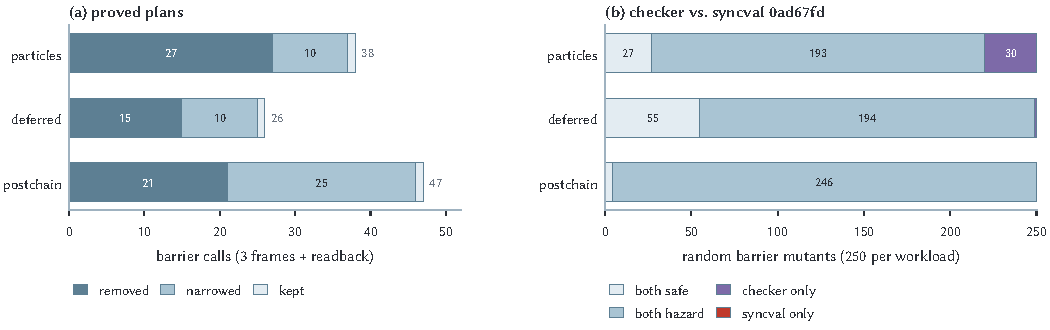
\includegraphics[width=\textwidth]{fig-barriers.pdf}
  \caption{\textbf{Barrier mutants and proved plans.} (a) Of 111 recorded barrier calls in three
  microbenchmarks, the proved plans of \S\ref{sec:elide} remove 63 and narrow 45; the 3 kept are host-readback
  barriers that the optimizer never touches. (b) The 750 random barrier mutants checked by \sys and by Khronos
  synchronization validation (lavapipe): no mutant is reported by validation only. ``Checker only''
  mutants remove the barrier after an \code{atomicAdd} (a write that validation still misses) or narrow a readback
  transition to a stage that excludes the copy. The released checker gives the same diagnostics on every mutant as
  the snapshot shown.}
  \label{fig:barriers}
\end{figure*}
We generated 750 random barrier plans for three headless single-queue workloads, each removing or narrowing barrier
structs within the recorded masks, and ran each under validation at the commit fixed for every later study
(full synchronization settings, lavapipe) and through the checker frozen for the first fresh study;
the release gives identical diagnostics on every mutant (Figure~\ref{fig:barriers}b, Table~\ref{tab:release}).
Mutant-level agreement is 95.9\%: 86 both safe, 633 both hazardous, 31 checker only and \textbf{none validation only}.
Thirty of the 31 checker-only mutants remove the barrier between an \code{atomicAdd} into a histogram and the
dispatch that reads it, a read-after-write race (an atomic read-modify-write is a write) that validation misses,
confirmed by a minimal reproduction; the last narrows a readback transition to \code{dstStageMask = ALL\_GRAPHICS},
which does not contain the copy that follows. These workloads have no semaphores, swapchain or host writes; the
whole-frame test below covers those.

\paragraph{Ray tracing and mesh shading}
Thirteen raw-Vulkan programs on one queue, run under validation (HEAD-max, lavapipe) and under \sys, give 12 equal
verdicts. In the thirteenth, a top-level build reads a bottom-level structure whose build is not made available to it;
only \sys reports it, because validation records only the instance buffer of a top-level build. Every correct program
is clean under both tools. The release gives the same codes and counts in all 15 modes of this test.

\paragraph{Whole-frame differential test}
\label{sec:eval-wholeframe}
A second harness covers what the mutants lack: three hand-written workloads of six frames each (an offscreen pass
blitted to the swapchain, an async-compute frame on two timeline semaphores, and a staging-ring upload with a shared
depth buffer), in five configurations with two or three frames in flight and, for the timeline workload, a second,
compute-only queue family with ownership transfers. In every frame the host waits on an earlier frame, writes mapped
memory, acquires and presents. A generator mutates semaphore waits and signals, per-frame indexing, fence waits,
presents, every barrier and both halves of each ownership transfer, for 1,251 programs in all. Each runs under \sys
and under validation (full synchronization settings) on lavapipe with a real X11 surface; the
multi-queue configuration ran on the Khronos mock driver, patched to give the second family a compute queue, where
validation analyses the submitted commands without executing them. Findings are normalized to (class, object) keys and
every disagreement is classified by explicit rules (Table~\ref{tab:wholeframe}).

\begin{table}[t]
\caption{Whole-frame differential test, 1,251 programs, regenerated and re-checked with the release (all 1,251
guarantee-eligible). Agreement: share of programs on which both tools report a finding or neither does. Pairs:
(program, object) for hazards, (program, finding) for all classes. Frozen: the checker frozen before the test (fresh).
The two release columns differ only in whether the \code{acquire-first-use} warning is scored as a hazard. Lower part:
the remaining disagreements of the middle column, by cause.}
\label{tab:wholeframe}
\small
\resizebox{\columnwidth}{!}{%
\begin{tabular}{@{}lrrr@{}}
\toprule
& frozen & \multicolumn{2}{c}{release} \\
\cmidrule(l){3-4}
first-acquire scored as hazard & -- & no & yes \\
\midrule
agreement, hazards & 88.4\% & 97.9\% & 98.3\% \\
agreement, all finding classes & 84.3\% & 95.4\% & 95.8\% \\
hazard pairs: both / \sys only / validation only & 1,132 / 17 / 322 & 1,440 / 32 / 14 & 1,454 / 65 / 0 \\
all pairs: both / \sys only / validation only & 1,270 / 413 / 1,199 & 2,353 / 478 / 116 & 2,367 / 511 / 102 \\
\midrule
\multicolumn{4}{@{}l}{\emph{reported by \sys only (478)}} \\
\multicolumn{3}{@{}l}{\quad host-write race; missing ownership acquire (validation limits)} & 205 + 3 \\
\multicolumn{3}{@{}l}{\quad same root cause under another object or code (key mapping)} & 201 \\
\multicolumn{3}{@{}l}{\quad model driver's acquire order; lavapipe hung or crashed} & 51 + 4 \\
\multicolumn{3}{@{}l}{\quad write-after-write without a destination access (strict reading)} & 14 \\
\multicolumn{4}{@{}l}{\emph{reported by validation only (116)}} \\
\multicolumn{3}{@{}l}{\quad unwaited acquire as a message of its own (both report the race)} & 75 \\
\multicolumn{3}{@{}l}{\quad surface minimum image count 3 on lavapipe vs.\ 2} & 23 \\
\multicolumn{3}{@{}l}{\quad first use of a never-presented image} & 18 \\
\bottomrule
\end{tabular}}
\end{table}

\emph{Fresh result and release.} The checker frozen before the test agreed with validation on 88.4\% of the
programs on hazards. The disagreements exposed six errors in \sys, all fixed since, each a case that validation caught
and \sys missed: a binary semaphore signalled again while a signal was pending was not reported; neither was a
timeline signal whose value did not increase; the sync2 transfer stages \code{COPY}, \code{BLIT} and \code{CLEAR} were
merged into \code{TRANSFER}; the stage mask of a sync2 semaphore signal was ignored; command buffers, fences and acquire
semaphores reused while pending were not reported; and grouping split one over-acquire site. We regenerated all 1,251
programs and checked them with the release (validation's stored verdicts are reused): agreement is 97.9\% on hazards,
and every program is guarantee-eligible. Of the 116 remaining validation-only finding pairs, 75 are an unwaited
acquire that validation reports as a message of its own while both tools report the resulting race, 23 come from
lavapipe's surface allowing one fewer held image, and 18 are first uses of a never-presented image, which the release
reports as an \code{acquire-first-use} warning; scored as a hazard, it leaves no validation-only hazard pair (98.3\%).
The traces, the per-program results and a script that re-checks them are part of the artifact.

\emph{What \sys adds, and what validation adds.} \sys alone reports 205 races between host writes and GPU reads of an
earlier frame still in flight, and three reads of an exclusive buffer on a queue family that never acquired it;
validation checks only that an acquire matches a pending release. Fourteen pairs are a modelling choice: \sys
requires a memory dependency for a write-after-write. The other way, validation's model of the acquire as an access
was what \sys lacked for never-presented images. Neither tool needs a race to manifest: on the mock driver,
validation gives the same findings as on lavapipe in 967 of the 989 completed single-queue runs.

\emph{Limits of this test.} The workloads are small and hand-written, the mutation catalogue is designed rather than
mined, there is one swapchain per program and no recreation, events or ray tracing, and the second queue family was
never executed concurrently. The programs use dynamic rendering, no framebuffer-local dependency, no descriptor
array and no host write after a device write, so they do not exercise those parts of the model. The key mapping can misattribute a disagreement within a class: 201 pairs are the same
root cause under another object or code. We claim no speed advantage: on these programs a lavapipe run with validation
takes a median 0.081\,s and \sys 0.092\,s. What \sys adds here is coverage.

\paragraph{Window measurements}
Of the 187 stored sample traces, 138 are periodic with a fence bound ($N = 1$ for 26, 2 for 85, 3 for 27). On them,
checking only the first $w + N + 2$ frames found 1,229 of the 1,262 normalized diagnostic sites of the full traces;
the 33 missing sites are \code{unmodelled-command} warnings from stubbed commands, and no race or protocol site was
missing. These are measurements on the traces. They are not instances of Theorem~\ref{thm:window}, whose bound $M =
w + p + \max(N, G+1) - 1$ the window analysis does not compute (\S\ref{sec:window}).

%% -------------------------------------------------------------------
\subsection{E2: Blind detection on \bench}
\label{sec:eval-bench}

\begin{figure}[t]
  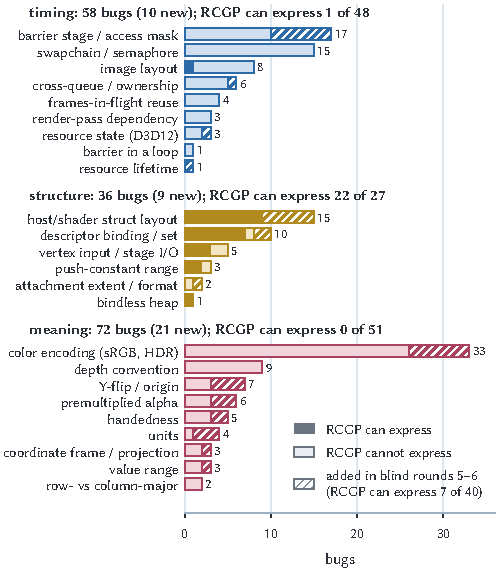
\includegraphics[width=\columnwidth]{fig-gpubugbench.pdf}
  \caption{\textbf{\bench.} 166 real bugs from 105 projects, by kind: the 126 bugs of the first collection
  (79 projects) and 40 collected fresh for blind rounds 5 and 6 (hatched). Filled bars are the first-collection bugs
  that \rcgp's contracts can express (23 of 126). This paper's guarantee concerns the timing bugs; the benchmark keeps
  all three kinds.}
  \label{fig:bench}
\end{figure}

\paragraph{The benchmark}
Existing GPU bug collections cover CUDA synchronization~\cite{wu2020simulee}, CUDA
numerics~\cite{rathnasuriya2025numerical}, shader compilers~\cite{donaldson2017graphicsfuzz,xiao2025shadiv} and
WebGPU implementations~\cite{wong2025webglitch}; none targets application graphics code. \bench follows the Defects4J
recipe~\cite{just2014defects4j}: we searched issue trackers by validation-message strings, fix phrases and
convention-related phrases, read every issue, pull request or commit page, and kept a bug only if it was real and lived
in application, engine or sample code. It has 166 bugs from 105 projects (Figure~\ref{fig:bench}) in three kinds:
\emph{timing} (synchronization), \emph{structure} (host/shader layout, bindings, interfaces) and \emph{meaning}
(semantic conventions). The first collection, 126 bugs from 79 projects (48 timing, 27 structure, 51 meaning), is the
basis of a taxonomy (\supp{H}) and of 74 distilled buggy/fixed reproductions in Slang and C++/Vulkan. Swapchain or
semaphore misuse accounts for 15 of its 48 timing bugs, and about half (24 of 48) span frames or queues. The other 40
bugs were collected fresh, each with a merged upstream fix, and reproduced blind for rounds 5 and 6.
\emph{Threats.} Validation-message queries favour Vulkan timing reports, most projects are small, root causes were
read from issue pages, and reproductions keep the upstream root cause but are not upstream code.

\paragraph{Protocol}
Before each round the checker was frozen (by source hash from round 3 on), and the outcome of every case was predicted
and timestamped before the run. Round 2 was written by a separate party that never ran the checker; rounds 3--6 were
written without reading checker code, and rounds 5 and 6 used bugs collected fresh from public trackers. After each
round, misses became general rules and the round's cases became development data.

\paragraph{Metrics}
The preregistered headline is \emph{strict paired-detection success}: a case counts only if its buggy variant reports
every expected diagnostic code \emph{and} its fixed variant reports nothing. It is stricter than bug-detection recall:
a real report under a different code, or any diagnostic on the fixed variant, is a failure. We keep it unchanged, and
add two measures whose case keys were fixed before any post-hoc re-run: \emph{root-cause detection} (the buggy
variant reports at least one timing diagnostic on the case's root-cause resource, whatever its code), and
\emph{fixed-variant diagnostics} (fixed variants that report anything).

\begin{table}[t]
\caption{Blind detection on \bench, as run: each round scored by the checker frozen for it (fresh). Timing: strict
paired-detection success and root-cause detection. Structure and meaning are outside the synchronization guarantee and
are given for completeness (strict). Fixed: fixed variants (all categories) with any diagnostic / with a timing
diagnostic. Pred.: predictions that held.}
\label{tab:blind}
\small
\resizebox{\columnwidth}{!}{%
\begin{tabular}{@{}lrrrrrr@{}}
\toprule
& \multicolumn{2}{c}{timing} & & & & \\
\cmidrule(lr){2-3}
Round (cases) & strict & root cause & struct. & meaning & fixed & pred. \\
\midrule
1 (17--29) & 3/7 & 4/7 & 1/2 & 2/4 & 1 / 1 & 13/13 \\
2 (30--44) & 4/7 & 4/7 & 2/4 & 0/4 & 2 / 0 & 13/15 \\
3 (45--59) & 3/6 & 3/6 & 1/3 & 0/6 & 0 / 0 & 14/15 \\
4 (60--74) & 3/5 & 4/5 & 1/3 & 0/7 & 8 / 5 & 13/15 \\
5 (75--94) & 5/6 & 5/6 & 0/5 & 0/9 & 2 / 1 & 17/20 \\
6 (95--114) & 3/4 & 4/4 & 1/4 & 0/12 & 1 / 0 & 14/20 \\
\midrule
total & \textbf{21/35} & 24/35 & 6/21 & 2/42 & 14 / 7 & 84/98 \\
Wilson 95\% & \textbf{44--74\%} & 52--81\% & 14--50\% & 1--16\% & & \\
\bottomrule
\end{tabular}}
\end{table}

\begin{figure}[t]
  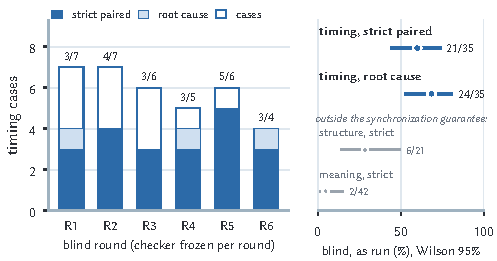
\includegraphics[width=\columnwidth]{fig-heldout.pdf}
  \caption{\textbf{Blind detection, as run.} Left: timing cases per blind round; strict paired-detection successes
  (dark), cases whose root cause was reported (light), all timing cases (outline). Right: pooled rates with Wilson
  95\% intervals. Structure and meaning are outside the synchronization guarantee (grey).}
  \label{fig:heldout}
\end{figure}

\paragraph{Results}
Table~\ref{tab:blind} and Figure~\ref{fig:heldout} give all six rounds. Strict paired-detection success on timing is
21 of 35 (60\%, Wilson 95\% interval 44--74\%), and root-cause detection 24 of 35 (69\%, 52--81\%). The three cases
with the root cause found but no strict success are 28 and 63, detected with a fixed variant that is not clean, and
98, a buffer returned to a decoder pool before the copy that reads it has finished, reported as a cross-queue race
instead of its expected \code{free-while-in-use} code. Eleven timing cases were missed entirely; the misses were
synchronization not yet modelled (semaphore stage masks, ownership pairs, object lifetime, stencil-only aspects) and
rules that did not fire.
Fourteen of 98 fixed variants (14\%, 9--23\%) drew some diagnostic, seven of them a timing diagnostic: cases 28 and 63
(above); 94, a structure case whose binding the checker charged at a stage whose entry point does not use it (the
release charges a binding only at the stages whose entry point uses it); and 65, 66, 68 and 69, which report a true race in the shared harness that the
cases' fixes do not touch (\supp{H}). The 21 of 35 pools six checkers, developed between rounds, so it
is evidence about the development sequence, not an estimate of one checker's recall. Predictions held in 84 of 98
cases, a statement about predictability, not coverage.

Outside the synchronization guarantee, the structure checks detected 6 of 21 structure bugs. An earlier component
that tried to infer semantic conventions detected 2 of 42 meaning bugs blind, and none of 21 in the last two rounds,
after two redesigns; we make no claim about conventions and keep those bugs in the benchmark (\S\ref{sec:limits}).

\paragraph{The release on \bench (post-hoc)}
After round 6, all 114 reproductions are development data. Re-run with the release, strict paired detection succeeds
on 29 of the 35 blind timing cases and the root cause is found in 33; 8 of the 98 blind fixed variants draw a
diagnostic, 6 of them a timing diagnostic (cases 61, 62, 65, 66, 68 and 69; \supp{H}). These numbers are tuned, not blind; the step from 21 and 24 as run is development between rounds.

\paragraph{\rcgp}
\label{sec:eval-rcgp}
For every first-collection bug we asked whether \rcgp's contract language rules it out through its typed API, from its
API and source, confirmed by 35 compile-only ports compiled by its own compiler. \rcgp can express 23 of the 126: 22
of 27 structure bugs, 1 of 48 timing bugs and none of the meaning bugs. Head to head on the 98 blind cases, \rcgp rules
out 17, \sys detects 29 under strict scoring (all categories), and together they cover 40: \rcgp alone catches 11,
all structure, and \sys alone 23. The comparison is one of scope, not a contest; ports, verdict changes and \rcgp's own
samples are in \supp{H}.

%% -------------------------------------------------------------------
\subsection{E3: The proved configuration on previously unchecked code}
\label{sec:eval-fresh}

\paragraph{Design}
Two studies measure the configuration the theorems cover (strict \code{UNDEFINED} transitions, conservative capture)
on workloads \sys had not been run on before, with prior exposure disclosed (below). For each, a protocol fixing the programs, the run length, the triage rules
and the metrics was written before the checker was frozen by source hash and before any program was checked; every
\code{check.json} carries the frozen hash. Each program ran unmodified under the model driver for 20 presents and was
checked in conservative capture (primary) and observed capture. Report groups were triaged by written, mechanical
rules into true bug, technicality, false alarm or \emph{unresolved} (the verdict depends on a reading of the
specification we cannot settle), and into two families: \emph{race} diagnostics, about unordered accesses, and
\emph{protocol} diagnostics, about the use of semaphores, fences and swapchain images. A group takes the most
consequential class of its members. A checker defect found during triage is not fixed in the frozen checker; it is
counted as it fell and fixed only for the next study. The baseline is synchronization validation
(all synchronization checks enabled) on lavapipe, on the same programs and number of presents, with two exceptions:
one wgpu program crashes under lavapipe and has no validation result, and the mpv runs could not be limited to 20
presents and play their test video to the end. Comparisons with validation are over the 56 programs it completed.

\emph{Study 1} froze a checker snapshot and ran 32 programs from four code bases: the Qt~6.4 rendering hardware interface (14 Qt Quick
3D and Qt Quick examples), wgpu (15 examples), Dear ImGui (2 Vulkan backends) and vkcube. \emph{Study 2} froze a
later snapshot, which fixed the three defects study~1 exposed and modelled two more commands, and ran 25 programs
from four others: GTK~4.14 (9 programs of its Vulkan renderer), vkmark (7 scenes), mpv~0.37 with libplacebo~6.338
(4 renderer configurations) and the GStreamer~1.24 Vulkan plugins (5 pipelines). The programs were chosen from a
bring-up run that recorded only whether a program starts and presents; programs that render only on demand or need a
compiled module were excluded, so the sample is conditioned on workloads this capture procedure can run and is not
representative of arbitrary applications. Prior exposure: Dear ImGui's Vulkan backend had been linked into two
earlier programs as an overlay, and a libplacebo change had been considered (and rejected) as an earlier benchmark
case; neither was checked. The protocols, the disclosures and every per-program number are in \supp{I}. All 57
programs were checked in both modes; 56 were grouped with the frozen checkers (Cost, below).

\begin{table}[t]
\caption{The proved configuration on previously unchecked code, as frozen (study 2: 24 of 25 programs grouped). Report groups true / technicality / false alarm
(/ unresolved) and the share that is true; causes: distinct root causes in the same classes.}
\label{tab:fresh}
\small
\resizebox{\columnwidth}{!}{%
\begin{tabular}{@{}llrrrr@{}}
\toprule
Study & family & conservative & true & observed & true \\
\midrule
1 (32) & race & 44 / 12 / 1270 & 3.3\% & 44 / 12 / 205 & 16.9\% \\
 & protocol & 86 / 0 / 701 & 10.9\% & 86 / 0 / 701 & 10.9\% \\
 & all & 130 / 12 / 1971 & 6.2\% & 130 / 12 / 906 & 12.4\% \\
 & causes & 5 / 3 / 4 & 41.7\% & 5 / 3 / 3 & 45.5\% \\
\midrule
2 (24) & race & 229 / 0 / 1048 / 13 & 17.8\% & \multicolumn{2}{l}{identical} \\
 & protocol & 31 / 0 / 0 & 100\% & \multicolumn{2}{l}{identical} \\
 & all & 260 / 0 / 1048 / 13 & 19.7\% & \multicolumn{2}{l}{identical} \\
 & causes & 11 / 2 / 2 / 2 & 64.7\% & \multicolumn{2}{l}{identical} \\
\bottomrule
\end{tabular}}
\end{table}

\begin{figure}[t]
  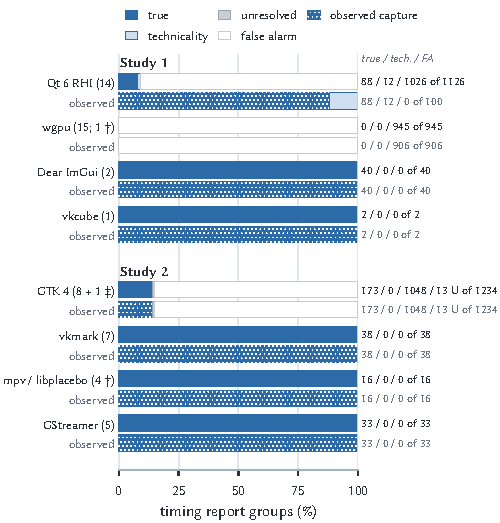
\includegraphics[width=\columnwidth]{fig-precision.pdf}
  \caption{\textbf{The proved configuration on previously unchecked code}, by code base: share of timing report groups
  that are true bugs, technicalities, unresolved and false alarms, with conservative capture (solid, the theorem's
  configuration) and observed capture (dotted). Each study's checker was frozen before the study's first run.
  \dag: programs outside the premises (an unmodelled command; one wgpu program, all four mpv programs).
  \ddag: \code{gtk\_path\_walk}, checked but not grouped (memory), not in the bar.}
  \label{fig:precision}
\end{figure}

\paragraph{Precision}
Table~\ref{tab:fresh} and Figure~\ref{fig:precision} give the results as frozen. They are not uniformly good, and we
report them as they fell. In study~1, 6.2\% of report groups were true. Two causes produced almost every false alarm.
Qt writes only the current frame's slot of each dynamic uniform buffer, after waiting for that slot's fence; the
conservative capture takes each host write to cover its whole page, which the slot in flight shares (1,026 groups,
all 14 Qt programs, none in observed capture). And three checker defects, a timeline counter query not treated as a
host wait, whole-image layouts treated as unbounded ranges, and a combined depth format treated as color, produced all
of wgpu's 945 groups. With observed capture and the three defects fixed, the same traces give 130 / 12 / 0, but that
number is post-hoc, which is why study~2 exists.
In study~2, 19.7\% of groups and 64.7\% of causes were true. vkmark, GStreamer and mpv produced 87 groups,
all true. Every false alarm is GTK's and has two causes. GTK's renderer binds all of a frame's images in one
descriptor array and selects one per draw instance through a vertex attribute; \sys charges a read to every written
element of a statically used binding, which is sound but here wrong 1,042 times, since only the dynamically used
descriptors count; the release removes this cause (\S\ref{sec:eval-release}). Six more groups are uploads into disjoint rectangles of one texture atlas, which \sys models per
subresource. In study~2 observed capture gives exactly the conservative result: on these code bases, the proof costs
no precision. Thirteen GTK groups are unresolved: they depend on whether a render pass's automatic layout transitions
are ordered with a later barrier and with each other, which the specification does not state (\S\ref{sec:limits}).

\paragraph{What a developer reads}
Grouping shrinks the output, but it is not one report per mistake. In conservative capture, the 28,370 group members
of study~1 fall into 2,113 groups and 12 causes, and the 189,900 of study~2 into 1,321 groups and 17 causes. A
developer of one program sees on average 3.7 groups per true cause in study~1 and 4.4 in study~2; only 4 of 35 and
25 of 59 program--cause pairs produce a single group. Most repetition comes from per-frame and per-image structure: a
Dear ImGui example recreates its swapchain every frame under the model driver and shows its one bug in 20 groups, and
GTK's missing render-before-present ordering appears in 15 groups per program. False-alarm causes repeat far
more (the descriptor-array over-approximation: up to 927 groups in one program). Cause-level numbers in this section are our manual consolidation,
not something the tool shows; we did not measure how long diagnosis takes.

\paragraph{From report to clean run}
To show the workflow end to end, we patched the source of every true cause in four projects (vkmark, GStreamer,
Dear ImGui, and SDL3 from E4), rebuilt each program with its original flags and re-ran it with the same command. There
are 11 source-patch cases covering nine causes: one per cause, plus one case per project that applies all of its
patches together (vkmark and GStreamer). We re-checked every patched run with the release in conservative capture
(\supp{I}). For each case, the patched run has no diagnostic of the repaired cause and no diagnostic kind the
original lacked, and every remaining diagnostic belongs to another listed cause. Applying all patches of a project
leaves 15 programs with no diagnostic in either capture mode and no synchronization-validation message: all seven
vkmark scenes (1,124 diagnostics before, five causes, 18 files changed), all five GStreamer pipelines (495 before, two
one-line patches), both ImGui examples (40 before, a 75-line deletion) and SDL's sprite test (166 before). With the
release, all 15 have no diagnostic in either capture mode, raise no model warning, and are guarantee-eligible in the
verified configuration; re-tracing each three more times gives the same result.
These are source repairs in the sense of \S\ref{sec:eval-bugs}: evidence through re-running, not through
Lemma~\ref{lem:repair}.

The same check tests upstream repairs. For each of the nine causes already changed upstream we distinguish an
\emph{initial fix attempt} (a commit that changes the implicated pattern but, re-run, leaves diagnostics of the
cause), a \emph{commit changing the pattern} (read in the source, not re-run) and a \emph{verified complete repair}
(re-run, no diagnostic of the cause). We re-ran vkmark's two commits. Both are initial fix attempts: the
uniform-buffer commit leaves 136 of the cause's 152 diagnostics, because it rewrites image $i$'s
buffer once acquire returns $i$, which does not show the host that the frame that read it has finished, and in one
scene it drops a fragment stage from a descriptor layout, which vkmark corrected later; the acquire commit
leaves 119 diagnostics, and validation still reports its semaphore error. The other seven are
commits changing the pattern.

\paragraph{Premises}
We report for each program whether a capture or coverage violation was \emph{detected}, which is weaker than
establishing every premise. Of the capture premises (\S\ref{sec:capture}), P1 (the trap is in effect) is checked; P2
(stores go through the returned mapping) is assumed, since no trace can show it; and P3 (one host order) is checked
only as far as the trap reveals, at the first store to each page between two calls. The model premises of
Table~\ref{tab:assume} are assumed. No program raised a capture warning. In the frozen runs, five programs used
commands the frozen checker did not model: wgpu's mipmap example (query result copies, which the second study's
checker models) and the four mpv configurations (timestamp queries, which have no memory effect on the checked
resources). The release reports, for each run, whether it is in the guarantee's domain
(Table~\ref{tab:release}).

\paragraph{What validation sees}
Validation found the same root causes as \sys in study~1 (5 shared, none unique to either tool). In study~2 the tools
share 10 true causes, and one is unique to \sys: vkmark rewrites its uniform buffer with \code{memcpy} every frame
without waiting for the frame that reads it, a host-write race that validation does not track. Validation is unique
on none, and it reported no synchronization false alarm in either study; it is silent on every false-alarm and
unresolved cause of \sys. Both tools report potential hazards implied by the declared synchronization without
needing them to manifest. On this evidence, \sys adds host-write capture and an explicit correctness argument for
its stated domain, not a larger set of findings on device work.

\paragraph{The bugs}
The 16 true causes of the two studies are listed in \supp{I}. For nine of them the project's current source has a
commit that changes the implicated pattern (Qt's acquire- and present-semaphore reuse, vkcube's present semaphore,
vkmark's acquire semaphore and its uniform-buffer race, libplacebo's barrier that does not chain to an external
semaphore wait, and GTK's three swapchain bugs). All nine commits predate our analysis, landing 11 to 27 months before
the studies, and five of them name an earlier issue report; they corroborate the triage and were not caused by us.
As shown above, two of them are initial fix attempts and the other seven were read, not re-run; \supp{I} lists, per
cause, the tested revision, the commit, its date and its label. Seven causes are still present in the current
sources: Dear ImGui transitions swapchain images before acquiring them; Qt makes a texture visible only to the vertex
stage and samples it in the fragment shader; vkmark reuses one present semaphore, its clear scene's barrier does not
chain to the acquire wait, and its depth image is shared across frames with only a color dependency; GStreamer waits
for the acquire semaphore at \code{BOTTOM\_OF\_PIPE}, so the wait blocks nothing, and makes a sampled image visible to
input-attachment reads only. Two of these, ImGui's and vkmark's present semaphore, already have open reports and
proposed fixes by other users.

%% -------------------------------------------------------------------
\subsection{The release on the studies' traces}
\label{sec:eval-release}
After the two studies we changed the checker in four ways: framebuffer-local dependencies are modelled with position
tokens (Definition~\ref{def:spec}); two layout transitions on one queue are exempt only if one is explicit (E5); a
descriptor-array read is narrowed to the elements its index bytes select when the guard conditions of
\S\ref{sec:guards} hold; and grouping has a memory budget. The release also reports the host-domain warning and each
run's eligibility (\S\ref{sec:eligible}). All numbers in this subsection are post-hoc: they re-check the traces the
studies recorded, with the release. On these traces the release loses no true group of the frozen runs.

\emph{Study 1} (32 programs, all grouped completely): in conservative capture, 130 / 10 / 2 / 1,026 groups (true /
technicality / unresolved / false alarm), 11.1\% true; in observed capture, 130 / 10 / 2 / 0, 91.5\% true. Every
false alarm is Qt's page-granular host capture. The two unresolved groups are pairs of automatic render-pass
transitions in two Qt programs, the question of \S\ref{sec:limits}. All 15 wgpu programs report nothing.

\emph{Study 2} (25 programs): grouping completes on 24 of them, which give 260 / 1 / 8 / 6 groups, so 94.5\% of these
275 groups are true (19.7\% when frozen). The 25th, \code{gtk\_path\_walk}, reaches the grouping budget and is reported
\emph{incomplete}: 35 site groups without repairs, of which 22 are true (the same three GTK causes), 12 unresolved and
1 a false alarm, with all 15,595 diagnostics kept; it is not in the 94.5\%. The false alarms of the 24 programs fall
from 1,048 groups to 6 because a draw that selects its texture with a flat per-instance index whose bytes the host
wrote, with no racing write, is charged only the elements those bytes select; every other indexing keeps the
over-approximation. The six that remain are texture-atlas uploads into disjoint rectangles of one image.

\emph{Domain.} On all 114 runs (57 programs, two capture modes) the release raises no host-domain warning. In
conservative capture all 57 runs are in the
guarantee's domain: checking completed, no unmodelled command has a memory effect (the timestamp queries of the four
mpv programs have none), and no host write relies on premise A-HOST. The observed-capture runs are outside the
verified configuration by definition. Checking is complete for all 57 programs; reporting is complete for 56, the
exception being \code{gtk\_path\_walk}.

\emph{Cost.} Checking one program in one capture mode takes 0.01--10\,s for vkmark, GStreamer and mpv and up to a
few minutes for the GTK programs (Table~\ref{tab:cost}). The largest, \code{gtk\_path\_walk} (308,815 recorded calls,
40,100 host writes in 20 frames), needs about 8\,GB to group; the frozen checker exceeded the container's 15\,GB, so
the frozen results of Table~\ref{tab:fresh} exclude it.

\begin{table}[t]
\caption{Cost on the largest study-2 programs, conservative capture, one core, with the checker frozen for study~2
and with the release: wall-clock seconds and peak resident
memory of the check and of grouping. $^\ast$The frozen checker's grouping was killed at the 15\,GB limit; the release's
grouping stops at its budget and reports \emph{incomplete}.}
\label{tab:cost}
\small
\setlength{\tabcolsep}{4pt}
\begin{tabular}{@{}lrrrr@{}}
\toprule
program, checker & check s & check MB & group s & group MB \\
\midrule
\code{gtk\_iconscroll}, frozen & 170 & 2,033 & 571 & 2,489 \\
\code{gtk\_iconscroll}, release & 118 & 1,685 & 75 & 268 \\
\code{gtk\_widget\_factory}, frozen & 51 & 770 & 37 & 132 \\
\code{gtk\_widget\_factory}, release & 50 & 752 & 23 & 70 \\
\code{gtk\_path\_walk}, frozen & 719 & -- & -- & $>$15,000$^\ast$ \\
\code{gtk\_path\_walk}, release & 469 & 7,487 & 1,620 & 8,353$^\ast$ \\
\bottomrule
\end{tabular}
\end{table}

%% -------------------------------------------------------------------
\subsection{E4: Earlier studies}
\label{sec:eval-real}

Before the verified configuration existed, earlier checker snapshots were run on sample collections, tutorials and
three engine pairs. These results are reported as they ran, each with the snapshot frozen for it; \supp{E} lists the
snapshots and \supp{F} every triaged group.

\paragraph{Development data: two sample collections and a render graph}
We ran all 99 SaschaWillems/Vulkan samples, the 49 Khronos\-Group/\-Vulkan-\-Samples that record work under the model
driver, and, once ray tracing and mesh shading were modelled, 9 further Khronos ray-tracing and mesh-shading samples,
unmodified for 10 frames (157 programs; the 27 ray-tracing, mesh-shading and compute samples we examined in detail are
these 9 and 18 of the 99 Sascha Willems samples), plus the 78 tests of the vuk render-graph library. Every report was
triaged against the specification and the source. These samples became development data as soon as we fixed the
false-alarm causes they revealed (at the study snapshot 53 of 154 Sascha Willems report groups and 164 of 271 Khronos
ones were false alarms). They yielded 26 root causes that we judge real, including six host-write races (T1--T6), a
semaphore signal submitted with \code{stageMask = 0} so that its first scope is empty (KS-1), the ray-traced storage
image transitioned with no source access in all nine Sascha Willems ray-tracing samples (SW-13) and three Khronos
ones, and a bug in vuk's own barrier derivation (VUK-1). Validation reports some of these and misses others; it cannot
see the host races.

\begin{table*}[t]
\caption{One diagnostic per kind of bug (shortened with ``...''), as the release reports it on the stored traces.}
\label{tab:diag-examples}
\scriptsize
\begin{tabular}{@{}p{0.11\textwidth}p{0.15\textwidth}p{0.70\textwidth}@{}}
\toprule
Kind & Source & Diagnostic \\
\midrule
Missing barrier & ks/dynamic\_rendering (K3) & \texttt{[timing] timing.missing-barrier: 'swapchain[0]' is written and then read on queue 'graphics0' with no barrier in between. at vkCmdBeginRendering @seq 179 (...) (load op LOAD of color attachment swapchain[0]); note: earlier access: vkCmdBeginRendering @seq 164 (...) (load op CLEAR ...)} \\
Host-write race & sw/dynamic\-uniformbuffer (T1) & \texttt{[timing] timing.cross-queue-race: 'buffer\#3' is written on 'host' and read on 'graphics0' with nothing ordering the two. at vkCmdDrawIndexed @seq 350 (...): set 0 binding 0; note: other access: host write to buffer\#3 (mapped memory\#4 +0x0), before call seq 607} \\
Present / acquire & sw/dynamicrendering\-multisampling (T9a) & \texttt{[timing] timing.wait-stage-scope: the layout transition of 'swapchain[0]' is not ordered after the earlier read on 'present:swapchain[0]': the semaphore wait that orders the queues only blocks later stages, and this barrier's first scope (TOP\_OF\_PIPE) does not chain to it. note: include the wait's stage in the barrier's srcStageMask (for an acquired swapchain image: COLOR\_ATTACHMENT\_OUTPUT)} \\
Ray tracing & sw/raytracing\-basic (SW-13) & \texttt{the earlier write (RAY\_TRACING\_SHADER, SHADER\_STORAGE\_WRITE) is not made available before the layout transition of 'image\#5' (to 'transfer\_src'): the transition is ordered after the write by an execution dependency (the first synchronization scope ALL\_COMMANDS holds RAY\_TRACING\_SHADER), but the barrier's first access scope does not hold the write: srcAccessMask (NONE) does not include SHADER\_STORAGE\_WRITE. ... fix: add SHADER\_STORAGE\_WRITE to srcAccessMask (with RAY\_TRACING\_SHADER in srcStageMask)} \\
Render graph & vuk test \emph{lift compute 2} (VUK-1) & \texttt{[timing] timing.barrier-scope: the barrier on 'buffer\#1' does not cover this access: the earlier written (TRANSFER, TRANSFER\_WRITE) and this read (COMPUTE\_SHADER, UNIFORM\_READ) are not both in its stage/access masks. at vkCmdDispatch @seq 40 (...): set 0 binding 1} \\
\bottomrule
\end{tabular}
\end{table*}

\paragraph{Tutorials and three engine pairs}
\label{sec:eval-engine}
Each of these studies, too, froze its checker and triage protocol before its first scored run, and each study's false
alarms were then fixed, so a study is fresh only for the checker frozen before it (Table~\ref{tab:engines}).
On Khronos' Vulkan-Tutorial and vulkan-guide, the checker found three bugs in vulkan-guide chapters 5--6 (VG-1 to VG-3); 12 of
its 13 technicality groups are one per-chapter pattern. On vkQuake and Diligent, the false alarms were mostly host
writes into per-frame halves of ring buffers charged to the whole buffer; the true groups are three bugs: vkQuake's
indirect-draw and index buffers are rewritten by the next frame's compute dispatches while the previous frame's draws
may still read them (VQ-1), its render pass has no outgoing dependency (VQ-2), and Diligent's state tracker does not
count depth writes as writes (VD-1). On SDL3 and bgfx, all 13 false alarms came from one checker defect (a semaphore
wait with stage mask \code{ALL\_COMMANDS} was not allowed to order a layout transition in the same batch); the true
groups are SDL-1 (Figure~\ref{fig:teaser}). On Granite and VulkanSceneGraph, the checker reported no false alarm; the five bugs
are VulkanSceneGraph's semaphores waiting at \code{BOTTOM\_OF\_PIPE} by default (VSG-1), unordered consecutive transfer
submits (VSG-2), and three bugs in its examples (VSG-3 to VSG-5); 3 of the 12 programs were unchecked because the
frozen checker aborted on push constants declared for \code{VK\_SHADER\_STAGE\_ALL}. Validation found one bug the
checker missed (VD-2, the first transition of a never-presented swapchain image), which a first-acquire rule added
after that study now reports; validation's 16
write-after-write hazards in Granite's ambient-occlusion chain, on images bound through descriptor update templates
that \sys does not model, show that \sys is incomplete.

\begin{table}[t]
\caption{Earlier studies: timing precision of the checker frozen before each study, on code it had never been run on. Groups: report
groups true / technicality / false alarm; ``true'' and ``actionable'' (true or technicality) are shares of groups.
Causes: distinct root causes, true / technicality / false alarm. Raw: share of raw diagnostics that are true.}
\label{tab:engines}
\small
\resizebox{\columnwidth}{!}{%
\begin{tabular}{@{}lrrrrr@{}}
\toprule
Study (programs) & groups & true & actionable & causes & raw \\
\midrule
Tutorials (43) & 11 / 13 / 1 & 44.0\% & 96.0\% & 3 / 2 / 1 & 96.0\% \\
vkQuake, Diligent (4) & 8 / 0 / 44 & 15.4\% & 15.4\% & 3 / 0 / 7 & 97.9\% \\
SDL3, bgfx (12) & 2 / 0 / 13 & 13.3\% & 13.3\% & 1 / 0 / 1 & 57.2\% \\
Granite, VSG (12; 9 checked) & 8 / 12 / 0 & 40.0\% & 100\% & 5 / 1 / 0 & 39.3\% \\
\bottomrule
\end{tabular}}
\end{table}

\paragraph{Re-running the earlier corpora (post-hoc)}
\label{sec:eval-posthoc}
We re-ran the earlier corpora in the verified configuration; all of it is post-hoc, and the full table is in
\supp{H}. Conservative capture finds what observed capture cannot, the same-value host-write races T2--T5 in four
Sascha Willems samples, and it costs false alarms where host memory is sub-allocated below page size while neighbours
are in flight (+24 groups in vulkan-guide, +23 in vkQuake and Diligent, whose result falls from 7 / 2 / 11 of 20
groups to 7 / 2 / 34 of 43). All 12 Granite and VulkanSceneGraph programs now run. \code{vsg\_depthpeel} reports one
group we leave unresolved: whether a render pass's automatic final transition, whose implicit outgoing dependency has
an empty second scope, is ordered before a later pass's load operation (\S\ref{sec:limits}); \sys reports the pair.
Of these corpora, 13 traces are archived; the release re-checks them without losing a diagnostic
(Table~\ref{tab:release}).

\paragraph{A disagreement in the accept direction}
On VSG-5, validation reports 19 cross-frame write-after-write pairs that \sys finds ordered, so here \sys's verdict
is the more permissive one, and a clean verdict could rest on it. The ordering is a chain from frame $k$'s depth store
through the \code{EXTERNAL}$\to$0 dependency of the library's window pass ($\mathsf{LATE\_FRAGMENT\_TESTS}$,
\code{DEPTH\_STENCIL\_ATTACHMENT\_WRITE}) into frame $k{+}1$'s depth transition. The specification states that the
first synchronization scope of such a dependency includes the commands submitted before the render pass, and that its
first access scope is limited by the source stage and access masks only, not to the pass's attachments (render-pass
chapter, external dependencies); with these clauses the chain exists. Validation itself accepts the same pair when the
window pass's dependency is replaced by a pipeline barrier with identical masks (minimal reproduction in \supp{F}),
which suggests that it applies an external subpass dependency only to the pass's own attachments. Since the cited text
decides the case, no accepted ordering in our results rests on an unresolved reading (\S\ref{sec:limits}).

\paragraph{The bugs}
\label{sec:eval-bugs}
Over all studies we judge 54 bugs to be real: 26 in the samples and vuk, 3 in the tutorials, 9 in the earlier engine
studies and 16 in the two fresh studies. This triage is ours. We prepared 11 historical dossiers, one for each of the
11 strongest bugs of the earlier studies (Table~\ref{tab:bugs}), each with the affected revision, the code, the frozen diagnostic, the
validation messages on the same frames where validation can see the bug, a specification argument with a concrete bad
schedule, a repair, and the result after the repair.

\emph{Three kinds of repair evidence.} We distinguish them because they carry different guarantees. A
\emph{synthesized repair} widens masks or inserts a barrier without a transition; Lemma~\ref{lem:repair} shows it adds
no race under the specification, and the grouper checks it on the recorded frame. A \emph{trace-checked repair} is
any edit applied to the recorded trace and re-checked on the whole frame by event pairs. A \emph{source repair}
changes the program, for example from one shared buffer to one per frame; it changes the program's resources and
accesses, is outside the lemma, and is evidence only through rebuilding, re-running and re-checking. The dossiers'
repairs are source repairs: after rebuilding and re-running, \sys's count on the bug is 0, validation's count is 0
where validation can see the bug, and no new diagnostic kind appears. Eight of the 11 dossiers are corroborated by
validation on the same resource and command pair; the other three are host-write races, which validation does not
track. VSG-3 and VSG-5 are in vsgExamples, not in the library. The dossiers are distinct from the 11 source-patch cases
of \S\ref{sec:eval-fresh}, which cover nine causes of the fresh studies (SDL-1 is in both). The dossier summary is in
\supp{G}.

\begin{table}[t]
\caption{The 11 historical dossiers. Syncval: validation reports the same resource and command pair (n/a: a host-write
race, which validation does not track). Repair: \sys count before $\to$ after, with the snapshot frozen for the third
engine study; validation in parentheses.}
\label{tab:bugs}
\scriptsize
\resizebox{\columnwidth}{!}{%
\begin{tabular}{@{}llllr@{}}
\toprule
Bug & Project & Class & Syncval & Repair \\
\midrule
KS-1 & Vulkan-Samples & signal with \code{stageMask = 0} & yes & 99 $\to$ 0 (11 $\to$ 0) \\
KS-3 & Vulkan-Samples & no barrier between two rendering instances & yes & 40 $\to$ 0 (8 $\to$ 0) \\
SW-T1 & Sascha Willems & host write to a UBO in flight & n/a & 500 $\to$ 0 \\
SW-T6 & Sascha Willems & host write after the compute submit & n/a & 2 $\to$ 0 \\
SDL-1 & SDL3 & host write to vertex buffers in flight & n/a & 166 $\to$ 0 \\
VUK-1 & vuk & render graph derives a storage read & yes & 1 $\to$ 0 (1 $\to$ 0) \\
VSG-1 & VulkanSceneGraph & semaphore waited at \code{BOTTOM\_OF\_PIPE} & yes & 19 $\to$ 0 (18 $\to$ 0) \\
VSG-3 & vsgExamples & no barrier, compute write to vertex input & yes & 58 $\to$ 0 (19 $\to$ 0) \\
VSG-5 & vsgExamples & depth clear vs.\ layout transition & yes & 120 $\to$ 0 (39 $\to$ 0) \\
VD-1 & DiligentCore & depth write not a write state & yes & 114 $\to$ 0 (14 $\to$ 0) \\
VQ-1 & vkQuake & indirect buffers rewritten in flight & yes & 302 $\to$ 0 (19 $\to$ 0) \\
\bottomrule
\end{tabular}}
\end{table}

%% ===================================================================
\section{Verified Barrier Transformations}
\label{sec:elide}

Because the checker decides hazard-freedom for the whole recorded frame, it can serve as the oracle of a barrier
optimizer. This is an application of the verifier, not a headline result; the measurements are summarized here,
with details in \supp{H}.

%% =====================================================================
%% elision.tex -- replaces the theorem and proof sketch of Section 8 (paper-wo/main.tex, from
%% "\begin{theorem}[Elision soundness]" through the "\end{proof}" that follows it). Keeps label thm:elide;
%% Proof: appendix-proofs.tex, \S app:elide.
%% =====================================================================
\begin{theorem}[Elision soundness on the recorded execution]\label{thm:elide}
Let $P$ be a plan that removes or narrows barrier structs and keeps every layout transition, and let $\tau_P$ be the
trace with the plan applied. Let $F^*$ be the strengthened frame, in which each transition is split into a struct that
ends at the transition, the transition itself and a struct that starts from it, and load and store operations are
accesses. Let $F^*(\tau_P)$ satisfy the premises of Theorem~\ref{thm:sound}. If
$\Hpw(F^*(\tau_P)) \subseteq \Hpw(F^*(\tau))$, where pairs are compared by event identity (call, command and access
index), then $\Hspec(\tau_P) \subseteq \Hpw(F^*(\tau))$. In particular, if the pairwise mode reports nothing on
$F^*(\tau)$, then $\tau_P$ is race-free, and Corollary~\ref{cor:sched} applies to the transformed run on the recorded
host path.
\end{theorem}

The proof (Appendix~\ref{app:elide}) has two steps. First, $F^*$ only adds events and removes exemptions, and its
split structs chain exactly as the original struct did, so every race of a trace is a race of its strengthened frame.
Second, Theorem~\ref{thm:sound} on $F^*(\tau_P)$ and the premise give the inclusion. The premise is checked on the final
plan, so the order of the greedy search does not matter. Two requirements of the theorem are easy to lose in an
implementation. The comparison must be by event pairs. A comparison by diagnostic text or site can hide a new pair
behind an existing report of the same site, for example when a command buffer is submitted twice. It must also use the
pairwise mode. The epoch mode reports only a subset (Lemma~\ref{lem:modes}), so ``no new epoch report'' does not
imply the premise.

\paragraph{Beyond the recorded frames}
The theorem covers the frames that were traced, and nothing more. Reusing a plan on later frames would need the run to
continue as the recorded one, and a runtime matcher that falls back safely when it does not. We do not claim such a
reuse guarantee. Two obstacles show why a simple matcher is not enough: draining the device queues at a mismatch does
not drain the presentation engine, which may still read an image whose transition the plan narrowed; and a host write
can land in mapped memory before the matcher sees the call that reveals the mismatch. The layer
\code{VK\_LAYER\_COVENANT\_elide} matches each barrier call by its recorded key and applies the plan only to the
recorded ordinals; runs that go beyond them are measurements, not instances of Theorem~\ref{thm:elide}.


\paragraph{Method and lesson}
A greedy search visits barrier calls in recording order and tries removal, then narrower masks built from the accesses
around each occurrence, keeping a candidate when the whole frame reports no new racing event pair. Barriers with
\code{HOST} stages, ownership transfers and barriers around unmodelled commands are pinned; layout transitions are
only narrowed. The premise is checked on racing event pairs, not on diagnostic keys: a key comparison lets one
existing witness hide new races (on one Khronos sample, a key-based plan adds 1,560 races under the reference
semantics). Likewise the strengthened frame charges the presentation engine's read of an image from its acquisition
on, not from its first present. A proof-licensed transformation is only as sound as the frame and the comparison its
premise is checked on.

\paragraph{Measurements}
\label{sec:eval-elide}
On three headless microbenchmarks we wrote with a full barrier after every pass, the plans remove 63 of 111 recorded
barrier calls and narrow 45 (Figure~\ref{fig:barriers}a); GPU-time measurements on one consumer GPU are in
\supp{H} and are not a claim of this paper. On eight unmodified samples the prover removes none of 414 per-frame barrier calls:
318 sit between accesses that already race and are pinned, and the other 96 are transitions it proved necessary.

%% ===================================================================
\section{Limitations}
\label{sec:limits}
We collect here the limitations stated next to the claims they affect.

\paragraph{Scope of the guarantee}
Every guarantee is relative to the executed host path, in the verified configuration, for runs in the domain the
checker reports (\S\ref{sec:eligible}). Other driver responses, swapchain recreation and error paths are not covered.
Multithreaded host code is modelled as one host queue; capture precondition P3 is checked only as far as the trap
allows, and Granite and vkQuake trigger its warning in every program, so their clean pairs are outside the premise.
Host reads of mapped memory are not events, aliasing of distinct resources is not modelled, and shader device-address
accesses, query results, the inputs of host acceleration-structure builds, descriptor update templates, push
descriptors and unmodelled commands are outside the model; unmodelled commands are reported. A host write whose
ordering after device work relies on the host-domain premise (A-HOST) draws a warning and takes the run out of the
domain; the model driver exposes only host-coherent memory, so non-coherent memory, which needs explicit flushes and
invalidations, is not covered.

\paragraph{The proofs}
The proofs are by hand, not mechanized, and relative to our transcription of the specification. The executable
reference shares that transcription; the differential tests test it, but only on small or designed programs. The
proofs are for the algorithm as pseudocode; the code is trusted and tested (\S\ref{sec:tcb}). The window theorem is
conditional on periodic continuation, which no trace establishes, and the window numbers we report are measurements.
Proposition~\ref{thm:complete} needs region-uniform traces, which the checker does not construct.

\paragraph{Protocol checks}
The present-semaphore check approximates ``after the acquisition's signal'' by host order and does not model present
fences. The over-acquire count is exact only for the recorded order.

\paragraph{Precision}
Conservative capture costs precision on programs that sub-allocate host-visible memory below page size while
neighbours are in flight (Qt: 1,026 false-alarm groups in study~1). The observed mode avoids it but is outside the
theorem. A descriptor-array read is narrowed only when its index is a flat vertex attribute with host-written,
race-free bytes; indices from push constants, uniforms, storage buffers or indirect draws widen to every element.
Images are modelled per subresource, so writes into disjoint rectangles of one atlas overlap. Precision on unseen
code therefore depends on the code base's idioms: in the frozen studies, five of eight code bases drew no false alarm
and three were dominated by them. Grouping the largest program stays within its memory budget only by reporting an
incomplete grouping, with site groups and no repairs.

\paragraph{Unresolved questions of the specification}
Whether a render pass's automatic final layout transition is ordered before later work by a dependency whose source
stage is \code{COLOR\_ATTACHMENT\_OUTPUT}, or by the transitions of a later render pass, is not stated by the
specification. \sys reads the text literally and reports these pairs; validation accepts them. Both readings lie in
the report direction for \sys: they can only add reports, never remove one, so no clean verdict depends on them. The
unresolved GTK and Qt groups and \code{vsg\_depthpeel} depend on this question, and we count none of them as bugs.
The one disagreement in the accept direction, VSG-5, is decided by the cited text (\S\ref{sec:eval-real}).

\paragraph{Evidence}
The evidence for the verified configuration is two studies of eight code bases, 20 frames each, on the paths a GPU-free
run takes. Each study is fresh only for the checker frozen before it; the release's results on the same traces are
post-hoc. The triage is ours, by written rules that we wrote. The blind \bench result pools six checkers, developed
between rounds. Recall on real code was not measured. The 54 bugs are our triage; 11 have historical dossiers, 8 of
them corroborated by validation, and nine causes had already been changed upstream before our analysis. The
barrier-removal measurements come from three microbenchmarks we wrote.

\paragraph{Semantic conventions}
An earlier component of \sys tried to infer conventions such as color encoding and units, and failed blind (2 of 42).
Conventions are outside this paper's claims.

%% ===================================================================
\section{Related Work}
\label{sec:related}

\paragraph{Graphics programming systems}
Spark~\cite{foley2011spark}, Spire~\cite{he2016spire}, Shader Components~\cite{he2017shadercomponents},
Slang~\cite{he2018slang} and staged metaprogramming~\cite{seitz2019staged} make shader code modular across stages and
with the host. Braid~\cite{sampson2017braid} types the CPU/GPU stage boundary.
RenderKernel~\cite{yang2024renderkernel} type-checks buffer usage and formats in a DSL.
Dr.Jit~\cite{jakob2022drjit} and Halide~\cite{raganKelley2013halide} hide scheduling behind a compiler.
\rcgp~\cite{sivaram2026rcgp} declares resource contracts and makes misuse unrepresentable at compile time; \sys
checks existing code across queues and frames, with a weaker, executed-path guarantee.

\paragraph{GPU verification and race detection}
GPUVerify~\cite{betts2012gpuverify}, Faial~\cite{cogumbreiro2021faial}, Kuiper~\cite{martinez2026kuiper},
Descend~\cite{kopcke2024descend}, Prism~\cite{bansal2026prism} and GPUMC~\cite{gpumc2025} reason inside kernels.
BARRACUDA~\cite{eizenberg2017barracuda}, iGUARD~\cite{kamath2021iguard} and SuperCollider~\cite{supercollider2026}
detect CUDA races dynamically. Tong et al.~\cite{tong2024gpuconsistency} formalize GPU memory models, including
Vulkan's. We use vector clocks~\cite{lamport1978time,mattern1989virtual} and FastTrack-style
epochs~\cite{flanagan2009fasttrack}. What is new is the event model of a graphics frame they run on, which treats the
presentation engine as a queue and host stores to mapped memory as captured accesses, and the proof that connects the
implemented algorithm to it.

\paragraph{Resource state and synchronization}
Typestate~\cite{strom1986typestate,garcia2014typestate,revocable2026typestate} and fractional
permissions~\cite{boyland2003fractional} underlie per-resource state. TypeSec~\cite{bicanic2025typesec} applies
typestate to OpenCL buffers. Render graphs~\cite{odonnell2017framegraph,amd2022rps} derive barriers at run time.
Synchronization validation~\cite{lunarg2021syncval} checks the declared synchronization of the submitted command
stream, across command buffers, queues and swapchain operations, on a real device or the mock driver; \sys
complements it with host-write capture, an explicit correctness argument for a stated domain, and checked repairs
and transformations. Blade~\cite{malyshau2026blade} measures how much dropping barrier tracking recovers, without a
correctness guarantee.

\paragraph{Bug benchmarks}
Defects4J~\cite{just2014defects4j} set the recipe. GPU-related collections cover CUDA~\cite{wu2020simulee,
rathnasuriya2025numerical}, shader compilers~\cite{donaldson2017graphicsfuzz,xiao2025shadiv}, WebGPU
implementations~\cite{wong2025webglitch}, WGSL uniformity~\cite{leejones2026uniformity} and visual glitches in canvas
games~\cite{macklon2022canvas}.

%% ===================================================================
\section{Conclusion}
\label{sec:conclusion}
\sys treats a graphics frame as what it is, a concurrent program, and checks its synchronization from one GPU-free run
of the unmodified program: host memory, presentation and overlapping frames in one specified order, with diagnostics
that name the failed scope test and repairs that are re-checked. For a run in its stated domain, which the checker
reports, an accepted trace is race-free under every device schedule consistent with its synchronization, for the
modelled accesses on the recorded host path, by a complete proof written by hand and relative to our transcription of
the specification. Blind, frozen checkers achieved strict paired detection on 21 of 35 timing bugs and found the root
cause of 24. On eight code bases not checked before, the frozen checkers found 16 true root causes, one of which
validation cannot see, with no false alarm on five code bases. On the same traces, the release reports 94.5\% of
report groups true on the 24 programs of the second study whose grouping completes. Patching nine of the causes makes
15 programs clean under both \sys and validation. What remains is to narrow sub-page host writes, to settle the open
questions of the specification, to measure recall on real code and to run on GPUs with several concurrent queues.

\bibliographystyle{ACM-Reference-Format}
\bibliography{refs}

\appendix
%% =====================================================================
%% appendix-proofs.tex -- proofs for formal.tex (Sections 4 and 5) and elision.tex (Section 8).
%% Defines: app:proofs, app:sound, app:abstraction, app:hostdom, app:guard, app:fast, app:precision, app:window,
%% app:elide, app:repair, app:counter.
%% =====================================================================
\providecommand{\Sc}[1]{\mathit{Sc}_{#1}}
\providecommand{\ASc}[2]{\mathit{ASc}_{#1}^{#2}}
\providecommand{\ESs}{\mathit{ES}^{\mathrm{src}}}
\providecommand{\ESd}{\mathit{ES}^{\mathrm{dst}}}
\providecommand{\AS}{\mathit{AS}}
\providecommand{\chainto}{\rightsquigarrow}
\providecommand{\mspecl}[1]{\ensuremath{\Rightarrow_{m}^{#1}}}
\providecommand{\ordl}[1]{\mathit{ord}_{#1}}
\providecommand{\Hpw}{\ensuremath{\Haz_C^{\mathit{pw}}}}
\providecommand{\Hep}{\ensuremath{\Haz_C^{\mathit{ep}}}}
\providecommand{\Hspec}{\ensuremath{\Haz_{\mathit{spec}}}}
\providecommand{\pc}[1]{\textsc{#1}}
\providecommand{\reach}{\hookrightarrow}
\providecommand{\posof}{\pi}
\providecommand{\Hstrict}{\ensuremath{\Haz_{\mathit{spec}}^{\mathit{dom}}}}

\section{Proofs}
\label{app:proofs}

The proofs refer to the algorithm of Figure~\ref{fig:alg} by procedure and line. Throughout, $\tau$ is fixed and the
algorithm runs in the verified configuration (no relaxation for transitions from \code{UNDEFINED}). An event is
\emph{processed} when \pc{Access} is called for it.

\paragraph{Notation}
For an event $e$ and a link $(D,c)$ we write $e \reach_x (D,c)$ if there is a chain $(D_1,c_1) \chainto \dots
\chainto (D_k,c_k) = (D,c)$ ($k \ge 1$) with $e \in \Sc{1}(D_1)$ and $c_1$ given by the class rule of
Definition~\ref{def:spec}, and $e \reach_m (D,c)$ if moreover $e \in \ASc{1}{\ell}(D_1)$ for every $\ell \in R(e)$. We
write $e \reach (D,c)$ for $e \reach_m (D,c)$ when $k(e) = \mathsf{W}$ and for $e \reach_x (D,c)$ otherwise, and drop
the class when it is $\mathsf{G}$. If $e \reach (D,c)$ and $(D,c) \chainto (D',c')$ then $e \reach (D',c')$, because
the intermediate dependencies of a chain need only chain. For a signal or a wait, the access scopes equal the
synchronization scopes, so $e \in \Sc{1}(\mathsf{Sig})$ gives $e \reach_m \mathsf{Sig}$. We say that a link $(D,c)$
\emph{holds} $u$ for source $e$ if $s(u)$ is in $D$'s second stage set restricted by $c$, and $\posof(u) = \posof(e)
\ne \bot$ when $c = \mathsf{L}$. Two facts about classes are used throughout. (C1)~A $\mathsf{G}$ link dominates the $\mathsf{N}$ and
$\mathsf{L}$ links of the same dependency: its restricted second stage set contains theirs and it holds without a
token condition, so it holds every access they hold, and every link they chain into is chained into from it in class
$\mathsf{G}$, which again dominates. (C2)~Signals and waits have class $\mathsf{G}$, whatever class the link before
them has.

Two facts about the trace translation are used repeatedly. (F1)~The structs of one barrier call are consecutive on
their queue, and only their transitions lie at their positions (W2). (F2)~A semaphore wait has an empty first stage set
and a signal an empty second stage set, so a barrier never chains into a wait, and a chain leaves a queue only through
a signal and enters one only through the paired wait.

%% -------------------------------------------------------------------
\subsection{Soundness (Theorem~\ref{thm:sound})}
\label{app:sound}

\begin{lemma}[Linearization]\label{lem:lin}
Positions on a queue are assigned in processing order, a wait is processed after its signal, and host operations are
processed in host order. Hence if $D \chainto D'$ then $D$ is processed before $D'$, and if $a \xspec b$ then $a$ is
processed before $b$.
\end{lemma}
\begin{proof}
Line~7 of \pc{Check} assigns $p(o) = \mathit{VC}[n][n]$ after incrementing it, once per operation, in queue order.
Line~3 processes a wait only after its name has been signalled. A chain step is either a step on one queue to a later
position, a step on the host to a later position, or a signal to its paired wait (W1 makes the pairing unique).
Each goes forward in processing order, and so does the first step $a \in \Sc{1}(D_1)$ ($p(a) < p(D_1)$) and the last
$b \in \Sc{2}(D_n)$ ($p(D_n) < p(b)$).
\end{proof}

\begin{lemma}[Chain state]\label{lem:chain}
Let \pc{Chain}$(e)$ have been advanced over the barriers of $q(e)$ up to some point. Call a link $(B,\mathsf{G})$
\emph{x-reached} if $g_x$ held at $B$ (line~7 of \pc{Advance}), $(B,\mathsf{N})$ x-reached if $l_x$ held, and
$(B,\mathsf{L})$ x-reached if $l_x$ held and $\lambda(B) = \mathsf{loc}$ (line~8); m-reached likewise with $g_m$,
$l_m$ (line~9).
(a)~If $(B,c)$ is x-reached then $e \reach_x (B,c)$ through a chain of barrier structs on $q(e)$.
(b)~If $(B,c)$ is m-reached then $e \reach_m (B,c)$, and $e$ is in the first access scope of the first struct of that
chain on every element of $R(e)$.
(c)~Conversely, if $e \reach_x (B,c)$ through barrier structs of $q(e)$ only, then $(B,c)$ or $(B,\mathsf{G})$ is
x-reached, and the same for m-reached.
For the chain of a wait record, the same statements hold with ``$e \in \Sc{1}(D_1)$'' replaced by ``$W \chainto D_1$''
for the wait $W$ (all its links have class $\mathsf{G}$), and the m-reached and x-reached sets coincide.
\end{lemma}
\begin{proof}
Invariant: when \pc{Advance} reaches struct $B$, $X_o$ is the union, over the x-reached links of earlier calls, of
their second stage sets restricted by class ($\mathsf{G}$ and $\mathsf{N}$), $X^L_o$ the same for the $\mathsf{L}$
links, $X_c[s]$ and $X^L_c[s]$ those over the current call with struct identity $s$, and $\mathit{snap}[v]$ the four
unions at the latest set of event $v$ since the chain started, deleted by a reset. The same holds for the $M$ sets and
m-reached links, whose ends $M_{\mathit{ends}}$ ($\mathsf{G}$, and $\mathsf{N}$ restricted to stages outside $F$) and
$M^L_{\mathit{ends}}$ ($\mathsf{L}$) keep the second access masks. The invariant holds initially (all sets empty, or
$X_o = M_o = E$ for a wait record, which stands for the wait's second stage set in class $\mathsf{G}$) and is kept by
lines~1--3 and~6--9, since a new call folds the current one into the earlier ones. Advancing incrementally is a left
fold over the barrier list, so it computes the same sets as one pass.

(a) by induction over the order in which links are reached. Write $X_f$, $X^L_f$ for the sets of line~3.
\emph{Base:} $d_x$ holds, so $e \in \Sc{1}(B)$: line~4 tests $p(e) < p(B)$ (the chain starts at the first barrier at
or after $p(e)$, and a transition is admitted only at its own struct), the stage, the call condition and, for an
event wait, that $\mathit{snap}[v]$ exists, which holds exactly when a set of $v$ lies between $e$ and $B$ without a
later reset, that is $p(e) < c_B$. The class rule of Definition~\ref{def:spec} enters $B$ locally exactly when
$\lambda(B) \ne \mathsf{glob}$ and $e$ is located, which is $\mathit{lo}$; line~6 then sets $l_x$ (classes
$\mathsf{N}$, and $\mathsf{L}$ if $\mathsf{loc}$) and otherwise $g_x$ (class $\mathsf{G}$). \emph{Step:} $X_f$ or
$X^L_f$ meets $\ESs(S_1)$. Then some x-reached link $(B',c')$ has its restricted second set meeting $\ESs(S_1)$, with
$p(B') < p(B)$, $B'$ not another struct of $B$'s call, and $p(B') < c_B$ for an event wait, so $(B',c') \chainto
(B,c)$ for the class $c$ that the rule gives: from $X^L_f$ ($c' = \mathsf{L}$) into a local $B$, classes $\mathsf{N}$
and $\mathsf{L}$, which is $l_x$; from $X_f$ ($c' \in \{\mathsf{G},\mathsf{N}\}$) or into a global $B$, class
$\mathsf{G}$, which is $g_x$. By induction $e \reach_x (B',c')$.

(b) is the same argument for line~9. Its base case $d_m$ adds to $d_x$ that $k(e) = \mathsf{W}$, $s(e) \in
\AS(S_1)$, $f(e) \in_{\mathsf{W}} A_1$ and $r_B = \ast$ or ($r_B = r(e)$ and $R_B \supseteq R(e)$), which is $e \in
\ASc{1}{\ell}(B)$ for every $\ell \in R(e)$. A transition is in both access scopes of its own barrier.

(c) by induction on the length of the chain, with the same case split read backwards: if $(B',c') \chainto (B,c)$ and
$(B',c')$ is x-reached, its restricted second set is in $X_f$ or $X^L_f$ (by the invariant; same call and struct, or
an earlier call, or the snapshot of an event wait with $p(B') < c_B$), and it meets $\ESs(S_1)$, so line~6 fires for
the class the rule gives. If only $(B',\mathsf{G})$ is x-reached, (C1) gives $(B,\mathsf{G})$.

For a wait record, $d_x = d_m = \mathit{false}$, the seeds of $X$ and $M$ are equal and the local sets start empty,
so only class $\mathsf{G}$ arises and lines~7 and~9 fire together.
\end{proof}

\begin{lemma}[Same queue]\label{lem:same}
Let $q(e) = q(u)$ and let line~4 or line~5 of \pc{Ordered} return \emph{ok}. Then $\ordl{\ell}(e,u)$ holds for every
$\ell \in O = R(e) \cap R(u)$.
\end{lemma}
\begin{proof}
All barriers in $\mathit{Bars}[n]$ precede $u$. \emph{Line~5}, execution mode: $s(u) \in X_{\mathit{tot}}$, so some
x-reached link $(B,c)$ with $c \in \{\mathsf{G},\mathsf{N}\}$ has $s(u)$ in its restricted second set (for $s(u) =
\bot$, only a $\mathsf{G}$ set of $\top$ contains it), hence it holds $u$ and $e \reach_x (B,c)$ by
Lemma~\ref{lem:chain}(a); or $\posof(u) = \posof(e) \ne \bot$ and $s(u) \in X^L_{\mathit{tot}}$, so an x-reached
$(B,\mathsf{L})$ holds $u$. Memory mode: some m-reached link holds $u$ with $u \in \ASc{2}{\ell}(B)$ for every $\ell
\in O$ (the test of \pc{Reaches}: $r_B = \ast$ or $R_B \supseteq O$, stage in the restricted set and in $\AS(S_2)$,
flag in $A_2$, and the token for an $\mathsf{L}$ end), and $e \reach_m (B,c)$ with $e$ in the first access scope on
all of $R(e) \supseteq O$ (Lemma~\ref{lem:chain}(b)).
\emph{Line~4}, $u = t_B$: $u$ is processed when $B$ is appended, so $B$ is the last barrier. If the chain reached $B$
last globally, then $e \reach (B,\mathsf{G})$ or $e \reach (B,\mathsf{N})$ and $t_B$ is in both scopes of its own $B$;
a transition is located, so an $\mathsf{N}$ link alone does not hold it, but the chain reached $B$ in class
$\mathsf{G}$ there, since line~8 adds no stage of $\mathsf{LT}$ to the global sets and the last global position is set
only by line~7. If it reached $B$ last locally, then $\posof(e) = \posof(u)$ and the $\mathsf{L}$ link holds $t_B$.
Otherwise $e \in \Sc{1}(B)$ directly (the test repeats the conditions of $\Sc{1}$, including the event cut and the
exclusion of other structs of the call and of transitions), in memory mode $e \in \ASc{1}{\ell}(B)$ on $O$, and, when
$B$ is entered locally from $e$, $\lambda(B) = \mathsf{loc}$ and $\posof(e) = \posof(u)$, so the one-link chain
$(B,\mathsf{L})$ holds $t_B$; when $B$ is not entered locally the link is $(B,\mathsf{G})$.
\end{proof}

\begin{lemma}[Relays]\label{lem:clock}
Assume W1. Let $\mathsf{Sig}(x,S)$ be processed on queue $q_s$ with relay $\rho$, let $e$ be an event on queue $m$,
and let $(t, \varphi) \in \rho[m]$ with $p(e) \le t$, where $\varphi = \bot$ or \pc{InSignal}$(e,\varphi)$ holds. Then
$e \reach \mathsf{Sig}$.
\end{lemma}
\begin{proof}
By induction on processing order, over the signals. An entry of $\rho$ is never created by $\sqcup$, which only keeps
or drops entries, so every entry of $\rho[m]$ was put there by one of the lines of \pc{Relay}$(q_s, p(\mathsf{Sig}),
S)$. \emph{Line~1}, the signal's own entry ($m = q_s$, $t = p(\mathsf{Sig})$): $e$ is an operation of $q_s$ other than
$\mathsf{Sig}$, so $p(e) < p(\mathsf{Sig})$. If $S = \top$, $e \in \Sc{1}(\mathsf{Sig})$ (every stage, $\bot$ and
transitions included), which is also the signal's first access scope. Otherwise $\varphi$ describes $\mathsf{Sig}$ and
Lemma~\ref{lem:insig} below gives $e \reach \mathsf{Sig}$. \emph{Lines~2--4}, an entry of the relay $\rho'$ of a wait
$W$ on $q_s$ processed before $\mathsf{Sig}$, whose signal $\mathsf{Sig}'$ was processed earlier still. By induction,
$e \reach \mathsf{Sig}'$, and $\mathsf{Sig}' \chainto W$ by W1. It remains to show that $W$ chains into $\mathsf{Sig}$,
possibly through barriers of $q_s$. Line~2: $S = \top$, and $W$'s second stage set has a stage other than $\mathsf{LT}$
(line~5 of \pc{Check} keeps no other wait), so it meets $\top$ and $W \chainto \mathsf{Sig}$. Line~3: $W$ has $E =
\top$, and $\ESs(S)$ has a stage other than $\mathsf{LT}$, so they meet. Line~4: $\pc{Chain}(W).X_{\mathit{tot}}$ meets
$\ESs(S)$. Either the seed $E$ meets it, and $W \chainto \mathsf{Sig}$; or some link $(B,\mathsf{G})$ that the wait
record's chain x-reaches has $\ESd(S_2)$ meeting $\ESs(S)$, so $W \reach_x B$ by Lemma~\ref{lem:chain} (wait-record
form) and $B \chainto \mathsf{Sig}$. The intermediate dependencies of a chain need only chain (Definition~\ref{def:spec}), so in
every case $e \reach \mathsf{Sig}$, and in memory mode the first link is still the one that holds $e$ in its first
access scope.
\end{proof}

\begin{lemma}[Signal filter]\label{lem:insig}
If \pc{InSignal}$(e,\varphi)$ holds for the masked signal $\mathsf{Sig}$ that $\varphi$ describes, and $e$ precedes it
on its queue, then $e \reach \mathsf{Sig}$.
\end{lemma}
\begin{proof}
Line~1: $e$ is not a transition and $s(e)$ is in the signal's first stage set, so $e \in \Sc{1}(\mathsf{Sig})$, which is
also its first access scope. Line~3: the chain of $e$ is advanced over the barriers before the signal. For a write,
some m-reached link $(B,c)$, of any class, has its restricted second stage set meeting the signal's first stage set,
so $(B,c) \chainto \mathsf{Sig}$, a link of class $\mathsf{G}$ by (C2), and $e \reach_m (B,c)$
(Lemma~\ref{lem:chain}(b)). For a read, the same with an x-reached link. This is why \pc{InSignal} tests the union of
the global and the local sets: a local chain followed by a signal is an ordinary chain.
\end{proof}

\begin{lemma}[Waits]\label{lem:viawait}
Assume W1. If \pc{ViaWait} returns true for $(e,u,\mathit{mem},O)$, then $\ordl{\ell}(e,u)$ holds for every $\ell \in
O$.
\end{lemma}
\begin{proof}
Let $m = q(e)$, $n = q(u)$. \emph{Line~1.} $\mathit{Full}[n][m] \ge p(e)$ means that some wait $W$ on $n$ processed
before $u$ has $E = \top$ and an unfiltered entry $(t, \bot) \in W.\rho[m]$ with $t \ge p(e)$ (line~6 of \pc{Check}).
By Lemma~\ref{lem:clock}, $e \reach \mathsf{Sig} \chainto W$, and $u \in \Sc{2}(W)$ because $W$ has every stage. A
transition is in $\Sc{2}$ of an earlier wait of every stage, and the access scope of a wait is its synchronization
scope. No other shortcut exists: in particular, a wait on a semaphore signalled by the host is accepted here only if
it has $E = \top$. \emph{Lines~2--6.} The record $w$ of a wait $W$ is used only if (line~3) its relay holds an entry
$(t,\varphi)$ for $m$ with $t \ge p(e)$ and $\varphi = \bot$ or \pc{InSignal}$(e,\varphi)$. Lemma~\ref{lem:clock}
then gives $e \reach \mathsf{Sig} \chainto W$, so $e \reach W$. Then: line~4, $u \in \Sc{2}(W)$ as above. Line~5, $u =
t_B$ and $W$'s chain reaches $B$, the last barrier on $n$, so $W \reach B$ (Lemma~\ref{lem:chain}) and $t_B$ is in both
scopes of $B$. Line~6, $s(u) \in E$ gives $u \in \Sc{2}(W)$, or $W$'s chain reaches $u$ as in Lemma~\ref{lem:same},
line~5. In memory mode the first link of the chain from $e$ is a signal, or a barrier that covers $R(e)$
(Lemma~\ref{lem:insig}), and the last link holds $u$ in its second access scope on all of $O$.
\end{proof}

\begin{proof}[Proof of Theorem~\ref{thm:sound}]
Let \pc{Ordered}$(e,u)$ return \emph{ok}, with $\mathit{mem} = (k(e) = \mathsf{W})$, which is the choice of
$\ordl{\ell}$. Line~2: both are on the host, and host order is an execution and memory order (A-HOST). Lines~4--5:
Lemma~\ref{lem:same}. Lines~6 and~8: Lemma~\ref{lem:viawait}. So $\ordl{\ell}(e,u)$ holds for all $\ell \in O$, that
is, $e \spec u$.

For the inclusion, let $\{a,b\}$ race at $\ell$, and let $e$ be the one that is processed first and $u$ the other. In pairwise
mode $e$ is never removed from any segment, and $u$'s segments partition $R(u)$, so $e$ is in the segment that holds
$\ell$. It is a candidate of \pc{Access}$(u)$: writes always are, and reads are when $u$ writes, which a conflict
requires. The pair is not exempt by E1--E4, so \pc{Ordered}$(e,u)$ is called. It cannot return \emph{ok}, since that
would give $\ordl{\ell}(e,u)$. Line~4 of \pc{Access} does not apply, because an E5 pair is exempt
and does not race. So line~5 reports the pair.

The locality of Definition~\ref{def:spec} enters this proof only through Lemmas~\ref{lem:chain} and~\ref{lem:same}: the
chain state distinguishes the three classes exactly as the definition does, and a local ending is accepted only with
equal tokens. Lemma~\ref{lem:clock} needs no change beyond (C2), because every relay entry passes through a signal, and
Lemma~\ref{lem:viawait} none, because a wait record's chain starts in class $\mathsf{G}$.
\end{proof}

%% -------------------------------------------------------------------
\subsection{From the run to the events (Corollary~\ref{cor:sched})}
\label{app:abstraction}

Model the run as the trace $\tau$ (A1) with its \emph{true} accesses $\alpha$ in place of the events. Each $\alpha$
has its exact stage, flag and byte or element set. The dependencies are those of $\tau$, and the true accesses are
ordered by Definition~\ref{def:spec} applied to them. A device access $\alpha$ is \emph{represented} by an event $a$ (A2)
if they have the same queue and position (that of the command), $R(a) \supseteq R(\alpha)$, $s(a) \in \{s(\alpha),
\bot\}$, $f(a) \in \{f(\alpha), \bot\}$, $k(a) = \mathsf{W}$ if $\alpha$ writes, and every exemption tag of $a$ is
also a true exemption of $\alpha$. A CPU store $\sigma$ is represented by a host write $w$ as in A2-H.

\begin{lemma}[Abstraction]\label{lem:abs}
If $a$ represents $\alpha$ and $b$ represents $\beta$, then for $\ell \in R(\alpha) \cap R(\beta)$,
$\ordl{\ell}(a,b)$ implies $\ordl{\ell}(\alpha,\beta)$. Hence, if $\alpha$ and $\beta$ race at $\ell$, then $a$ and
$b$ race at $\ell$.
\end{lemma}
\begin{proof}
Scope membership is monotone in the direction we need. $\bot$ lies only in a set of every stage, which contains
$s(\alpha)$. A $\bot$ flag lies only in a mask that contains \code{MEMORY\_READ} or \code{MEMORY\_WRITE}, which contains
$f(\alpha)$. Access-scope membership at an element $\ell$ depends on $\ell \in R_B$, not on the rest of the region, and
positions are equal. So $a \in \Sc{i}(D)$ implies $\alpha \in \Sc{i}(D)$, and $a \in \ASc{i}{\ell}(D)$ implies
$\alpha \in \ASc{i}{\ell}(D)$, and a chain for $a,b$ is a chain for $\alpha,\beta$. If $\alpha$ writes, so does $a$, so
$\ordl{\ell}(a,b)$ uses the memory relation whenever $\ordl{\ell}(\alpha,\beta)$ does, and the memory relation implies
the execution relation. For a store $\sigma$ represented by $w$, A2-H states directly that $w$ and $\sigma$ have the
same predecessors and successors. It holds for page capture because $w$ sits between the two host calls that
bracket $\sigma$, where the host queue has no other operation, and host-queue orderings depend only on the position
relative to host signals and waits. For the race: $\ell \in R(a) \cap R(b)$, one of $a,b$ writes, and they are not
exempt, because a claimed exemption would be a true one. Neither $\ordl{\ell}(a,b)$ nor $\ordl{\ell}(b,a)$ holds,
since either would order $\alpha,\beta$.
\end{proof}

\begin{proof}[Proof of Corollary~\ref{cor:sched}]
By Lemma~\ref{lem:abs}, a race of covered accesses gives a race in $\Hspec(\tau)$, which is empty. The pairwise case
follows from Theorem~\ref{thm:sound} and the epoch case from Lemma~\ref{lem:fast}. For a device schedule consistent
with $\tau$'s synchronization, an ordered pair executes in that order with the required availability and visibility,
by the specification's definition of the dependencies.
\end{proof}

%% -------------------------------------------------------------------
\subsection{Index guards (Lemma~\ref{lem:guard})}
\label{app:guard}

The specification counts a descriptor as accessed only if an invocation \emph{dynamically uses} it, that is, evaluates
an access chain into the array with its index; the layout and synchronization requirements attach to that access. So
it suffices to show that in every schedule consistent with $\tau$, every invocation of $d$ indexes the array only with
elements of $I(d)$.

\begin{proof}[Proof of Lemma~\ref{lem:guard}]
Let $V$ be the attribute bytes that $d$ fetches (the words of vertices or instances $\mathit{first}, \dots,
\mathit{first}+n-1$ at the recorded offset and stride), let $r$ be $d$'s vertex-input read, which covers $V$ and
carries $g$, and let $S$ be the position of $d$'s submission in host order.

\emph{Step 1: in every schedule the fetch returns the bytes rebuilt at $S$.} By C5 no device command writes $V$ and no
image is bound on it, so the only writes to $V$ are host stores, which A2-H represents as host write events $w$ at the
call boundary of each store, over every byte of each written page. Consider such a $w$ on $V$. If $w$ and $r$ are
unordered, they race, so the race is reported: in pairwise mode by Theorem~\ref{thm:sound}; in epoch mode against $r$,
or against a later read that stands in for $r$ and inherits its guard, or against a host write that $r$ was compared
with and that $w$ precedes in host order, by Lemma~\ref{lem:fast}. A reported pair with $r$ or its stand-in fails $g$
(C6), contradicting the premise; a reported pair of $r$ and an earlier host write likewise. If $w$ is ordered before
$r$ and recorded before $S$, its bytes are in the rebuilt contents, since contents are rebuilt from every record before
$S$ in host order (one host thread, P3, checked per memory by C4). If $w$ is ordered before $r$ and recorded after
$S$ (for example through a host-signalled timeline value), then when $r$ is checked, $w$ or a later host write that
supersedes it is a live write entry on $V$ recorded after $S$, which fails $g$ (C6). If $r$ is ordered before $w$, $w$
does not affect what $r$ reads. Hence the fetch returns the rebuilt bytes, which C4 requires to be recorded for all of
$V$.

\emph{Step 2: the shader maps them into $I(d)$.} By C1 and C2 the index of every access chain into the array is, on
every path, a constant or the index chain applied to the attribute value delivered to the invocation: a flat fragment
input receives the provoking vertex's output, which the vertex shader sets to the chain applied to the attribute on
every path (an output not set on some path, or set through a derived pointer, makes the index unknown, and the binding
is widened). The analysis follows local variables and pointer parameters through stores, loads and calls and joins
over all paths, ignoring branch conditions, which can only add values. Attribute fetch of a 32-bit integer format at
the recorded stride, offset and input rate of a non-indexed direct draw (C2, C3) is a function of $V$. So every index
lies in $I(d)$, and by C7 none is out of range.

\emph{Step 3: the dropped events stand for no access.} The elements outside $I(d)$ are not dynamically used in any
schedule, so their events correspond to no access of the run, and the remaining events still represent every access
as A2 requires. Lemma~\ref{lem:abs} and Corollary~\ref{cor:sched} apply to the narrowed event set.

\emph{No circularity.} Whether $g$ holds depends on the checker's verdicts, which depend on the event set, which
depends on which guards hold. The conditions C5 and C6 mention only events on $V$, which are buffer bytes, and the
happens-before order. The events a guard adds when it fails are image reads (C8), and accesses create no dependencies
in Definition~\ref{def:spec}. So neither the events on $V$ nor any ordering changes when conditional reads are added or
removed, and the set of failing guards is the same in every run; the checker reaches it by re-running with the failed
guards widened. The executable reference defines $\Hspec$ with the same rule, and the property tests of
$\Hspec \subseteq \Hpw$ include guarded frames.
\end{proof}

%% -------------------------------------------------------------------
\subsection{Host-domain operations (Proposition~\ref{prop:hostdom})}
\label{app:hostdom}

\begin{proof}[Proof of Proposition~\ref{prop:hostdom}]
Since no error is reported, Theorem~\ref{thm:sound} and Lemma~\ref{lem:fast} give $\Hspec(\tau) = \emptyset$. Let $e$ be a
device write and $u$ a later host write that conflict; then $e \spec u$, and we show that $e$ is host-domain ordered
before $u$.

\emph{Pairwise mode.} \pc{Access}$(u)$ compares $u$ with $e$, \pc{Ordered} returns \emph{ok}, and since no warning is
reported \pc{HostDomain}$(e,u)$ holds: the fresh chain of $e$, advanced over the barriers of $q(e)$ up to $t =
\mathit{Full}[\mathit{host}][q(e)]$, m-reaches a link $(B,c)$ that holds a host access at \code{HOST\_READ} or
\code{HOST\_WRITE} on all of $O$. By Lemma~\ref{lem:chain}(b), $e \mspecl{\ell} (B,c)$ for every $\ell \in O$, and $B$
has $\mathsf{HOST}$ in its second stage and access stage sets and a host access in its second access mask ($\mathsf{HOST}$
is outside $F$, so the class does not matter). $\mathit{Full}[\mathit{host}][q(e)] = t$ means that a host wait $W$
before $u$ has an unfiltered relay entry $(t,\bot)$ for $q(e)$, so by Lemma~\ref{lem:clock} every operation of $q(e)$
at a position up to $t$, $B$ among them, is in the first scope of a chain of signals and waits of every stage that ends
at $W$; and $u \in \Sc{2}(W)$, because a host wait holds every later host event. This is the chain from $B$ that
Definition~\ref{def:hostdom} asks for.

\emph{Epoch mode.} Suppose $e$ is not compared with $u$. Then $e$ was dropped before $u$ was processed, by an access $v$
that stands in for it, and we show by induction on drops that $v$ carries the domain operation over to $e$. If $v$ is
a host write, it dropped $e$ only with \pc{Ordered}$(e,v)$ = \emph{ok} and no warning (a warning marks the pair
\emph{premise}, which keeps $e$), so $e$ is host-domain ordered before $v$ by the pairwise argument, and the chain
from $B$ to $v$'s host wait also reaches $u$, which follows $v$ in host order. If $v$ is a device write ordered after
$e$ (D1), or a write that supersedes $e$ (D2), then, by the induction, $v$ is host-domain ordered before $u$ through
some $B$, possibly on another queue. For D1, $e \mspecl{\ell} v$ and $v \mspecl{\ell} (B,c)$ compose as in
Lemma~\ref{lem:trans}, with $B$ treated as an access at stage $\mathsf{HOST}$: $e \mspecl{\ell} (B,c)$. For D2,
Lemma~\ref{lem:subst} gives $e \mspecl{\ell} (B,c)$ directly. A transition $v$ is a D1 drop. Shadow entries are
compared with $u$ as in Lemma~\ref{lem:fast}. In every case $e$ is host-domain ordered before $u$.
\end{proof}

The test is conservative in two ways that the property test of the checker exercises: a domain operation on another
queue is credited only through a stand-in, and in pairwise mode not at all; and a domain operation reached only
through stage-masked signals is not credited. On random frames with one and two device queues, every pair that the
pairwise mode warns about has its host write flagged (by a warning or a hazard) in epoch mode, and the epoch mode adds
no warning.

%% -------------------------------------------------------------------
\subsection{The epoch mode (Lemmas~\ref{lem:modes} and~\ref{lem:fast})}
\label{app:fast}

\begin{proof}[Proof of Lemma~\ref{lem:modes}]
\pc{Ordered} reads only the clocks, wait records, barrier lists and chains, and none of them depends on the
mode. Every candidate of the epoch mode, including shadow and $\mathit{hid}$ entries, is an earlier event that
overlaps $u$ and conflicts with it, so it is also a candidate in pairwise mode. The exemption test and the R-LT
test are the same in both modes.
\end{proof}

The epoch mode removes an entry $e$ from a segment $\varsigma \subseteq R(u)$ in three ways. (D1)~The write $u$ is
ordered after it: \pc{Ordered}$(e,u) = $ \emph{ok}. (D2)~The write $u$ supersedes the write $e$. (D3)~The read $u$
replaces the read $e$ of the same key $\kappa$. The proof needs two facts about the definition.

\begin{lemma}[Transitivity]\label{lem:trans}
Let $\ell \in R(a) \cap R(v) \cap R(x)$. If $a \xspec v$ and $v \xspec x$ then $a \xspec x$. If $a \mspecl{\ell} v$ and $v
\mspecl{\ell} x$ then $a \mspecl{\ell} x$.
\end{lemma}
\begin{proof}
Host order is transitive, and a host event before (after) the first (last) host dependency of a chain is in its
scope, so host-order steps compose with chains. Otherwise take chains $C_1 = D_1 \dots D_n$ for $(a,v)$ and $C_2 =
D'_1 \dots D'_k$ for $(v,x)$, with $v \in \Sc{2}(D_n) \cap \Sc{1}(D'_1)$. In memory mode $a$ is in the first access
scope of $D_1$ and $x$ is in the second access scope of $D'_k$ at $\ell$.

\emph{$v$ is not a transition.} $D_n$ and $D'_1$ are on $q(v)$ with $p(D_n) < p(v) < p(D'_1)$. Both stage sets contain
$s(v)$, or both are $\top$ if $s(v) = \bot$, so they meet. By (F1), no access lies between two structs of one call, so
they are not two structs of one call. If $D'_1$ is an event wait, $p(D_n) < p(v) < c_{D'_1}$. Hence $D_n \chainto
D'_1$ and $C_1C_2$ is a chain.

\emph{$v = t_B$.} By Definition~\ref{def:spec}, $D_n$ is $B$ or a wait $W$ of every stage before $B$, and $D'_1$ is $B$
or a signal $\mathsf{Sig}$ of every stage after $B$. (i)~$D_n = D'_1 = B$: concatenate and share $B$. (ii)~$D_n = W$ and
$D'_1 = \mathsf{Sig}$: $W$'s second set is $\top$ and meets $\top$, so $W \chainto \mathsf{Sig}$. (iii)~$D_n = W$ and
$D'_1 = B$: if $k \ge 2$ then $D'_2$ follows $B$ on $q(B)$ (by F2, $D'_2$ is not a wait) or is a signal there. Its
first stage set meets $B$'s second set, so it has a stage other than $\mathsf{LT}$ and $W \chainto D'_2$; event cuts
carry over, since $p(W) < p(B)$. Use $C_1 D'_2 \dots D'_k$. If $k = 1$, then $x$ follows $B$ on $q(B)$, so $x \in
\Sc{2}(W)$, which equals $\ASc{2}{\ell}(W)$, and $C_1$ alone orders $a$ before $x$. (iv)~$D_n = B$ and $D'_1 =
\mathsf{Sig}$: if $n \ge 2$, $D_{n-1} \chainto B$, so $D_{n-1}$'s second set has a stage other than $\mathsf{LT}$ and
$D_{n-1} \chainto \mathsf{Sig}$ ($D_{n-1}$ precedes $B$ on $q(B)$ by F2), so use $D_1 \dots D_{n-1} C_2$. If $n = 1$,
$a$ precedes $B$ on $q(B)$, so $a \in \Sc{1}(\mathsf{Sig})$, which equals the signal's first access scope, and $C_2$
alone orders $a$ before $x$. In every case the first link keeps $a$ in its first (access) scope and the last link keeps
$x$ in its second, so the memory statement follows too.

\emph{Classes.} It remains to check that the concatenated chain has classes that still hold $x$ for source $a$. The
chain for $(v,x)$ starts at $D'_1$ in the class that $v$ enters it with: locally if $D'_1$ is local and $v$ is
located. The chain for $(a,v)$ ends at $D_n$ in a class $c_n$ that holds $v$. If $c_n = \mathsf{G}$, the
concatenation enters $D'_1$ in class $\mathsf{G}$, which by (C1) dominates whatever class $v$ entered it with, so
every later link of $C_2$ has a dominating counterpart and $x$ is held without a token condition. If $c_n =
\mathsf{N}$, $s(v) \notin F$, so $v$ is not located and enters $D'_1$ in class $\mathsf{G}$, as does the
concatenation. If $c_n = \mathsf{L}$, then $\posof(v) = \posof(a) \ne \bot$ and $v$ is located; the concatenation
enters $D'_1$ from an $\mathsf{L}$ link, which by the class rule gives the same classes as entering it from the located
event $v$, so $C_2$'s classes are unchanged, and an $\mathsf{L}$ ending of $C_2$ holds $x$ for source $v$, that is with
$\posof(x) = \posof(v) = \posof(a)$, so it holds $x$ for source $a$. In the transition cases (i)--(iv) the shared or
bridging dependency is $B$ itself, a wait or a signal; waits and signals are $\mathsf{G}$ by (C2), and for (i) the
same argument applies at $B$.
\end{proof}

\begin{lemma}[Substitution]\label{lem:subst}
Let $e$ and $u$ be events on one queue with $p(e) < p(u)$, equal stage, kind and position token, neither a transition
nor in a barrier call, and let $\ell \in R(e) \cap R(u)$. If $u \xspec x$ then $e \xspec x$. If moreover $f(e) = f(u)$ and $u
\mspecl{\ell} x$, then $e \mspecl{\ell} x$.
\end{lemma}
\begin{proof}
For every dependency $D$ with $p(D) > p(u)$, membership in $\Sc{1}(D)$ depends on queue, stage, call, and $p < p(D)$ and
$p < c_D$, all of which $e$ shares with $u$ or satisfies a fortiori. Membership in $\ASc{1}{\ell}(D)$ adds the stage,
the flag and $\ell \in R_B$. Whether $D$ is entered locally depends only on the stage, and an $\mathsf{L}$ ending
compares the source's token, which $e$ and $u$ share. Host order is transitive. Without equal tokens the lemma fails:
an $\mathsf{L}$ chain from $u$ can order an access at $u$'s position that no chain from $e$ orders.
\end{proof}

\begin{proof}[Proof of Lemma~\ref{lem:fast}]
Let $\{e,x\}$ race at $\ell$, with $e$ processed first. We show that \pc{Access}$(x)$ reports a pair that contains $x$.
Let $\varsigma$ be the segment of $x$ that holds $\ell$. Say that $v$ \emph{covers} $e$ for $x$ if $v$ is processed
before $x$, $\ell \in R(v)$, $v$ conflicts with $x$, $v$ and $x$ are not exempt by E1--E4, and $\ordl{\ell}(v,x)$
implies $\ordl{\ell}(e,x)$. A \emph{cover sequence} is $e = v_0, v_1, \dots, v_k$ in which each $v_{j+1}$ covers $v_j$
for $x$, each $v_j$ with $j \ge 1$ covers $e$ for $x$, and, whenever $v_{j+1}$ is a transition, $v_j \in
v_{j+1}.\mathit{hid}$.

\emph{Invariant.} At every point between the processing of $e$ and of $x$, there is a cover sequence whose last element
$v_k$ is \emph{live} for $x$. That is, it is in $\mathit{Wr}_\varsigma$, or in $\mathit{Rd}_\varsigma$ (then $x$
writes), or it is the entry of a shadow record $(v_k, d) \in \mathit{Sh}_\varsigma$ whose dominator $d$ is exempt
from $x$ by E1--E3. Right after $e$ is processed, $k = 0$ and $e$ is in $\mathit{Wr}_\varsigma$ or
$\mathit{Rd}_\varsigma$. Since $e$ and $x$ conflict, $x$ writes if $e$ reads. The invariant can be broken only when an
access $u$ removes $v_k$ from $\varsigma$.
\begin{itemize}
\item (D1) $u$ writes, has no atomic mode, and \pc{Ordered}$(v_k,u) = $ \emph{ok}, so $\ordl{\ell}(v_k,u)$ by Theorem~\ref{thm:sound}. If $x$ is
  not exempt from $u$ by E1--E4, append $u$: it is in $\mathit{Wr}_\varsigma$, it conflicts with $x$, and
  $\ordl{\ell}(u,x)$, a memory order because $u$ writes, gives $\ordl{\ell}(v_k,x)$ by Lemma~\ref{lem:trans}, which
  uses the memory relation if $v_k$ writes and the execution relation if it reads. If $u$ is a transition, $v_k$ is
  added to $u.\mathit{hid}$. If $x$ is exempt from $u$ by E1, E2 or E3, then $u$ has a command, scope or instance, and
  \pc{Drop} records $(v_k, u)$ in the shadow list, so $v_k$ stays live for $x$. $x$ cannot be exempt from $u$ by E4,
  because $u$ has no atomic mode: line~9 of \pc{Access} never drops an entry at an atomic access, except by
  supersession (D2).
\item (D2) $u$ supersedes $v_k$: same queue, stage, flag, kind, scope, instance, load/store marker, atomic mode and
  token, neither a transition nor in a call. By Lemma~\ref{lem:subst}, $u$ covers $v_k$ unless $x$ is exempt from $u$ and
  not from $v_k$. Since the tags for E2--E4 are equal, that can only be E1, and then $u$ has a command and \pc{Drop}
  shadows $v_k$.
\item (D3) $u$ reads with the key $\kappa$ of $v_k$, which includes the token, so $v_k$ reads and $x$ writes. $\mathit{Rd}_\varsigma[\kappa]$
  becomes $[u]$ or $[u, o]$, where $o$ is the first entry of the old list whose command differs from $u$'s. The old list
  is ordered newest first. If $x$ is not exempt from $u$, append $u$ (Lemma~\ref{lem:subst}, execution part). Otherwise,
  since the key fixes E2--E4, $x$ is exempt by E1, so $u$ has a command $c = \mathit{cmd}(x) \ne
  \mathit{cmd}(v_k)$, and $o$ exists. Either $o = v_k$, which then stays, or $o$ is newer than $v_k$ with the
  same key and a command other than $c$, and we append $o$.
\item A shadow record is pruned when its dominator's command, scope and instance are no longer current on its queue.
  By W2, no later access can then be exempt from the dominator by E1--E3, so the record is not live for $x$.
\end{itemize}
In every case each new element covers $e$, by composing the implications.

\emph{Conclusion.} At \pc{Access}$(x)$, $v_k$ is a candidate. Consider \pc{Ordered}$(v_k,x)$. If it is \emph{ok},
then $\ordl{\ell}(v_k,x)$ by Theorem~\ref{thm:sound}, hence $\ordl{\ell}(e,x)$, contradicting the race. If it is not
\emph{ok} and the pair is not an E5 pair, then $(v_k,x)$ is reported. Otherwise line~4 adds
$v_k.\mathit{hid}$, which contains $v_{k-1}$ and overlaps $x$ at $\ell$, and we repeat with $v_{k-1}$. If $v_{k-1}$
was already compared, its verdict is \emph{ok}, which contradicts the race as before, or reported, or R-LT again. The
descent ends at the latest at $v_0 = e$. There \pc{Ordered}$(e,x)$ is not \emph{ok}, and the pair is not an
E5 pair, which would be exempt. So $(e,x)$ is reported. In all cases $x$ is in a reported pair.
\end{proof}

%% -------------------------------------------------------------------
\subsection{Precision (Proposition~\ref{thm:complete})}
\label{app:precision}

\begin{lemma}[Clock completeness]\label{lem:clockc}
Assume that no signal has a stage mask other than $\top$. If $e \reach_x W$ for a processed wait $W$ whose second
stage set has a stage other than $\mathsf{LT}$, then the clock $c$ joined at $W$ has $c[q(e)] \ge p(e)$, and $W$'s relay
holds an unfiltered entry $(t, \bot) \in W.\rho[q(e)]$ with $t \ge p(e)$.
\end{lemma}
\begin{proof}
Induction on the number of semaphore pairs in the chain. The last pair is $\mathsf{Sig} \chainto W$, with $\mathsf{Sig}$
on $q_s$. Every signal has $S = \top$, so \pc{Relay} returns at its line~2 with unfiltered entries only. If $q(e) =
q_s$, then $c[q_s] = p(\mathsf{Sig}) > p(e)$, and the signal's own entry is $(p(\mathsf{Sig}), \bot)$. Otherwise, by
F2, the chain enters $q_s$ through a wait $W'$ that precedes $\mathsf{Sig}$ there and chains onward, so its second set
has a stage other than $\mathsf{LT}$. By induction its clock has $c'[q(e)] \ge p(e)$ and its relay an unfiltered entry
$t' \ge p(e)$. $\mathit{VC}[q_s] \ge c'$ from then on, and $\mathit{RA}[q_s]$ keeps an unfiltered entry for $q(e)$ of at
least $t'$, because $\sqcup$ keeps the largest one; line~2 of \pc{Relay} merges $\mathit{RA}[q_s]$ into $\mathsf{Sig}$'s
relay.
\end{proof}

\begin{proof}[Proof of Proposition~\ref{thm:complete}]
$\Hspec \subseteq \Hpw$ is Theorem~\ref{thm:sound}. For the converse, let $(e,u)$ be reported. They conflict, are not
exempt, and are not an E5 pair, and \pc{Ordered}$(e,u)$ is not \emph{ok}. Suppose $\ordl{\ell}(e,u)$
for every $\ell \in O$. Fix $\ell_1 \in O$ and a chain $C$ for it. By region uniformity (ii), a barrier whose region
contains $\ell_1$ contains $R(e)$ if $e$ is in its first access scope at $\ell_1$, and contains $R(u) \supseteq O$ if $u$
is in its second. If $C$ contains no semaphore pair, it consists of barriers on $q(u)$ and Lemma~\ref{lem:chain}(b,c)
shows that \pc{Chain}$(e)$ m-reaches (x-reaches) its last barrier, so line~4 or~5 returns \emph{ok}. Otherwise let $W$
be the last wait of $C$. By F2, the rest of $C$ consists of barriers on $q(u)$. By Lemma~\ref{lem:clockc}, which applies by (i), $\mathit{VC}[q(u)][q(e)] \ge p(e)$,
so line~7 does not return \emph{race}, and $W$'s relay holds an unfiltered entry at or after $p(e)$, so line~3 of
\pc{ViaWait} examines $W$'s record, and it returns true at line~4 ($E = \top$), line~5 (the wait chain reaches $B$ by
Lemma~\ref{lem:chain}(c)) or line~6 ($s(u) \in E$, or the wait chain reaches the last barrier, which covers $O$).
In each case \pc{Ordered} returns \emph{ok}, a contradiction. Hence $\ordl{\ell}(e,u)$ fails for some $\ell \in O$, and
$\ordl{\ell}(u,e)$ fails too, since by Lemma~\ref{lem:lin} it would have $u$ processed first. So $(e,u)$ races at $\ell$.
\end{proof}

\paragraph{The split trace $\tau^\sharp$}
For each resource $r$, the regions of the barrier structs on $r$ generate a finite Boolean algebra of element sets.
Replace every event $a$ on $r$ by one event $a|_P$ for each atom $P$ of that algebra that meets $R(a)$, with region $R(a)
\cap P$, at consecutive positions and with $a$'s other attributes and tags. Then $\tau^\sharp$ is region-uniform. No
dependency lies between the parts, so no scope or chain changes, and access-scope membership at $\ell$ is that of $a$.
The parts of one access are pairwise disjoint and never conflict. Hence $a|_P$ and $b|_{P'}$ race at $\ell$ in
$\tau^\sharp$ if and only if $\ell \in P \cap P'$ and $a, b$ race at $\ell$ in $\tau$. W1 and W2 carry over.
By the proposition, the pairwise mode on $\tau^\sharp$ reports exactly the parts of the races of $\tau$ when (i) holds.

%% -------------------------------------------------------------------
\subsection{Periodic executions (Theorem~\ref{thm:window})}
\label{app:window}

Write $\mathit{call}(o)$ for the host call that appended $o$, and order calls by host order.

\begin{lemma}[Locality, W.1]\label{lem:loc}
Under P-MONO, every dependency of a chain from $a$ to $b$ was appended by a call in $[\mathit{call}(a),
\mathit{call}(b)]$. Hence whether two events are ordered, and whether they race, is the same in $\tau^\infty$ and in
any prefix of it that contains both, and it is preserved by any map that preserves queues, program order,
attributes, tags and pairing on the calls of that interval.
\end{lemma}
\begin{proof}
On one queue, operations are appended in host order. By P-MONO, a wait is appended after its signal. So every chain
step goes forward in host order, as do $a \in \Sc{1}(D_1)$ and $b \in \Sc{2}(D_n)$. The event cut of an event wait
$D$ matters only through whether a set lies between $a$ and $D$, which is again inside the interval. Under P-MONO no
wait of a prefix lacks its signal, so the prefix drops no operation.
\end{proof}

\begin{lemma}[Retirement, W.2]\label{lem:ret}
Let $a$ and $b$ be events, neither on a presentation queue, with $\mathit{call}(a)$ before $\mathit{call}(b)$, $b$ in a
frame $j \ge w$ and $\mathit{fr}(a) \le j - N$. Then $a \xspec b$ and $a \mspecl{\ell} b$ for every $\ell$.
\end{lemma}
\begin{proof}
If $a$ is on the host, then $b$ is on the host (host order) or in a batch submitted after $a$. In the latter case, the
host signal of that submission has $a$ in its first scope, and the submission wait has $b$ in its second (transitions
included). If $a$ is on a device queue $q$, then by the definition of $N$ the host has waited, before the first
submission or host access of frame $j$, on a $\top$ signal of $q$ that follows $a$. That signal holds $a$ in its first
scope, it chains into the host wait, and the host wait chains into every later host dependency, in particular into
the submission of $b$'s batch, whose wait holds $b$, or it holds the host event $b$ itself. All links are signals and
waits, whose access scopes are their synchronization scopes.
\end{proof}

\begin{lemma}[Presentation, W.3]\label{lem:pres}
Assume P-WSI and P-MONO. Let $b$ be a device write to a swapchain image $i$, held under the acquire $A_b$ and ended
by the present $P_b$. Let $\rho_A$ be the presentation-engine read appended at $A_b$ and $\rho_P$ the one appended at
$P_b$. If $b$ races an engine read $\pi$ of $i$, then $b$ races $\rho_A$ or $\rho_P$.
\end{lemma}
\begin{proof}
All operations of the presentation queue of $i$ are reads of $i$ and signals and waits of every stage. Between $\rho_A$
and the operations of $P_b$, the queue holds only $A_b$'s signals, because an image is not acquired twice without a
present in between. If $\pi$ precedes $\rho_A$ on that queue or is $\rho_A$: $\rho_A \xspec b$ fails, because otherwise
the chain starts at a signal of every stage after $\rho_A$, which also holds $\pi$, and so $\pi \xspec b$.
$b \mspecl{\ell} \rho_A$ fails by Lemma~\ref{lem:loc}, since $\rho_A$ is appended before $b$. So $b$ races $\rho_A$.
Otherwise $\pi$ is $\rho_P$ or follows it. $b \mspecl{\ell} \rho_P$ fails, because otherwise the chain ends at a wait
of every stage before $\rho_P$, which also holds $\pi$. $\rho_P \xspec b$ fails by Lemma~\ref{lem:loc}. So $b$ races
$\rho_P$.
\end{proof}

\begin{proof}[Proof of Theorem~\ref{thm:window}]
Let $\{a,b\}$ race in $\tau^\infty$, with $\mathit{call}(a)$ first. \emph{Distance (W.4).} If neither is a
presentation-engine event, then $\mathit{fr}(b) - \mathit{fr}(a) \le N - 1$ by Lemma~\ref{lem:ret}, or both lie in
the first $w$ frames. Otherwise, by P-WSI one of them is an engine read and the other a device write $b'$ to the same
image. By Lemma~\ref{lem:pres}, $b'$ races $\rho_A$ or $\rho_P$, which lie within $G$ frames of $b'$ by the definition
of $G$. In both cases there is a witness race $\{a',b'\}$ of frame distance at most $D - 1$, which has an event in
common with $\{a,b\}$. \emph{Translation.} While $\mathit{fr}(a') \ge w + p$, the calls from $\mathit{call}(a')$ to
$\mathit{call}(b')$ lie in frames $\ge w + p$, so $\sigma^{-1}$ maps them onto frames $\ge w$, preserving everything
Lemma~\ref{lem:loc} needs, and $\{\sigma^{-1}a', \sigma^{-1}b'\}$ is a race. After finitely many steps, $\mathit{fr}(a')
\le w + p - 1$ and $\mathit{fr}(b') \le w + p + D - 2 = M - 1$. By Lemma~\ref{lem:loc}, this witness is a race of the
first $M$ frames, which are those of $\tau$. Conversely, a race of the first $M$ frames is a race of $\tau^\infty$ by
Lemma~\ref{lem:loc}. The last sentence of the theorem follows with Theorem~\ref{thm:sound} and
Corollary~\ref{cor:sched}.
\end{proof}

\paragraph{Why a fence does not bound the presentation engine}
In the encoding, the engine's read of a presented image is the pair $\rho_P$ (after the present's waits) and $\rho_A$
(at the next acquire of that image, after it waits on the present's completion). A frame fence is a signal on a device
queue. Neither read is in its first scope, because no chain runs from the presentation queue to the device except
through an acquire's signal. So a fence wait proves nothing about them, and $N$ cannot bound them. This is the
reason for the separate parameter $G$ and for Lemma~\ref{lem:pres}.

%% -------------------------------------------------------------------
\subsection{Elision (Theorem~\ref{thm:elide})}
\label{app:elide}

$F^*$ splits each transition $t_B$ into a struct $B_1$ with $B$'s first stage, access and region masks and a second
stage set $\{\mathsf{LT}\}$, a transition use $\lambda_B$ at stage $\mathsf{LT}$, and a struct $B_2$ with first stage
set $\{\mathsf{LT}\}$ and $B$'s second masks. All three have $B$'s call and struct identity. $F^*$ also turns load and
store operations into accesses without the E3 exemption. Identify $\lambda_B$ with $t_B$.

\begin{lemma}[Conservativity of $F^*$]\label{lem:fstar}
For events $a,b$ of $\tau$ and every $\ell$, $\ordl{\ell}(a,b)$ in $F^*(\tau)$ implies $\ordl{\ell}(a,b)$ in $\tau$.
Hence $\Hspec(\tau) \subseteq \Hspec(F^*(\tau))$ under the identification.
\end{lemma}
\begin{proof}
$\mathsf{LT}$ lies in a stage set only if the set names it, so $\top$ does not contain it. $B_1$'s second set
therefore meets only $B_2$'s first set, and conversely. $B_1 \chainto B_2$ is allowed, because they share their
struct identity. $D \chainto B_1$ if and only if $D \chainto B$, and $B_2 \chainto D$ if and only if $B \chainto D$.
For events other than transitions, $\Sc{1}(B_1) = \Sc{1}(B)$, $\Sc{2}(B_2) = \Sc{2}(B)$, and the same holds for the
access scopes. Replacing each $B_1 B_2$ in a chain of $F^*(\tau)$ by $B$ gives a chain of $\tau$ with the same end
scopes. $\lambda_B$ is in the scopes of $B_1$ (second) and $B_2$ (first) only, and $t_B$ is in both scopes of $B$, so
orderings of $\lambda_B$ map to orderings of $t_B$. For the races: $F^*$ removes exemptions and adds events, but adds
no ordering among the events of $\tau$.
\end{proof}

\begin{proof}[Proof of Theorem~\ref{thm:elide}]
Let $\{a,b\} \in \Hspec(\tau_P)$. The plan removes or narrows only barrier structs and keeps every transition, so the
events of $\tau_P$ are those of $\tau$, identified by (call, command, access index). By Lemma~\ref{lem:fstar},
$\{a,b\} \in \Hspec(F^*(\tau_P))$. By Theorem~\ref{thm:sound} applied to $F^*(\tau_P)$, $\{a,b\} \in
\Hpw(F^*(\tau_P))$. By the premise, $\{a,b\} \in \Hpw(F^*(\tau))$. The premise is checked on the final plan, so the
order of the greedy search is irrelevant.
\end{proof}


%% -------------------------------------------------------------------
\subsection{Repair monotonicity (Lemma~\ref{lem:repair})}
\label{app:repair}

\begin{proof}[Proof of Lemma~\ref{lem:repair}]
\emph{Events.} Widening masks adds no access, and an inserted barrier without a transition adds a dependency but no
access event; layouts and regions are unchanged, so the transitions are the same. Hence $\tau$ and $\tau_r$ have the
same access events, identified by (call, command, access index), with the same resources, regions and kinds.

\emph{Scopes grow.} Write $M \sqsubseteq M'$ when every mask of a dependency is contained in the corresponding mask of
its repaired version. The execution scopes $\ESs$, $\ESd$ and the access scopes $\AS$ are monotone in the masks
(each is a union over named stages or flags, possibly expanded to logically earlier or later stages). So for the
repaired dependency $D'$ of $D$: $\Sc{1}(D) \subseteq \Sc{1}(D')$, $\Sc{2}(D) \subseteq \Sc{2}(D')$, and the same for
the access scopes. All other dependencies are unchanged.

\emph{Chains persist.} $D_1 \chainto D_2$ requires that the second synchronization scope of $D_1$ meets the first of
$D_2$ (and, within one call, the struct-identity condition, which a repair does not change). Both scopes only grow,
so every chain of $\tau$ is a chain of $\tau_r$, with end scopes that contain the original ones. An inserted barrier
only adds dependencies and therefore chains.

\emph{Orderings persist.} Execution ordering $\xspec$ and memory ordering $\mspec$ of two events are defined by the
existence of a chain whose first scopes contain the earlier event (and, for $\mspec$, whose first access scope
contains it) and whose last scopes contain the later one. By the two previous steps, every witness in $\tau$ is a
witness in $\tau_r$. Queue-order, semaphore, fence and host orderings are untouched. So $a \spec b$ in $\tau$ implies
$a \spec b$ in $\tau_r$.

\emph{Races.} A race is a conflicting pair, at least one a write, with overlapping regions, not ordered either way.
Conflict and overlap depend only on the events, which are the same, and every ordered pair of $\tau$ stays ordered.
Hence every race of $\tau_r$ is a race of $\tau$: $\Hspec(\tau_r) \subseteq \Hspec(\tau)$.

\emph{Implicit dependencies.} A render pass without an explicit $\mathsf{EXTERNAL}$ dependency has an implicit one.
The grouper widens it to a dependency whose masks contain the implicit masks, which is a widening in the sense above.
A repair that replaced the implicit dependency by an explicit one with fewer stages or flags would not be; the
grouper never emits one.
\end{proof}

%% -------------------------------------------------------------------
\subsection{Minimal frames}
\label{app:counter}

Each frame below is a regression test of the released checker. Each isolates one case in which a plausible
shortcut in the algorithm would accept a race; the frames show why the corresponding lines of
Figure~\ref{fig:alg} are needed. For each we give the pairwise result, the epoch result and the result of the
executable reference semantics.
\begin{itemize}
\item \textbf{Relay through a masked signal.} Compute: write \code{buf} (compute shader), $\mathsf{Sig}(a)$. Graphics:
  $\mathsf{Wait}(a, \text{vertex shader})$, $\mathsf{Sig}(b, \text{compute shader})$. Transfer: $\mathsf{Wait}(b)$,
  read \code{buf} (copy). The wait's second set does not meet the signal's first set, so no chain exists and the
  pair races. Relaying the compute queue's clock entry unfiltered through $\mathsf{Sig}(b)$ would accept it. The
  checker builds the relay of $\mathsf{Sig}(b)$ only from waits whose chain meets its first scope (\pc{Relay},
  line~4), so all three report the race. The host relay (a masked signal waited on by the host, which then submits)
  is handled in the same way.
\item \textbf{Host-signalled wait.} Host: submit, write \code{buf}, then signal value $t{=}5$ from the host. Graphics:
  submission wait, $\mathsf{Wait}(t{=}5, \text{fragment shader})$, read \code{buf} (vertex shader, uniform read).
  The write is ordered only into the fragment stage, so the pair races. Treating the wait as a submission would
  accept it; \pc{ViaWait} has no such shortcut (line~1 uses only full waits). All three report the race.
\item \textbf{Atomic stand-in.} One queue: fill \code{counter}; barrier transfer $\to$ compute; compute atomic
  add; fragment atomic add. The fill and the fragment add race. If the epoch mode dropped the fill at the compute
  add, the fragment add, which is exempt from the compute add by E4, would be compared with nothing. The checker does
  not drop an entry at an atomic access (\pc{Access}, line~9), so all three report the race.
\item \textbf{Token stand-in.} One render pass: a fragment-shader sampled read of image $A$, a fragment-shader
  input-attachment read of $A$ (position token $\pi$), a by-region barrier from the input-attachment read to the
  color-attachment write, and a color-attachment write of $A$ (token $\pi$). The local link orders the input read
  before the write, but not the sampled read, which has no token, so the sampled read and the write race. If the two
  reads shared an epoch read key, the input read would stand in for the sampled read and the race would be missed.
  The read key and \pc{Supersedes} include the token (\pc{Access}, line~10), so both modes and the reference report
  the race, whether or not the two reads come from one command.
\item \textbf{Host write after a fence only.} Device: write \code{buf} (transfer). Host: wait on the fence, then
  write \code{buf} through a mapped pointer. Without a barrier whose second scope holds a host access, the host write
  relies on premise A-HOST (Definition~\ref{def:hostdom}); both modes emit the warning
  \code{timing.premise-host-domain}, and the frame is not guarantee-eligible. Adding a barrier from the transfer
  stage to the host stage with \code{HOST\_WRITE} removes the warning.
\item \textbf{Region cut.} Write $[0,100)$; global barrier; writes $[0,50)$ and $[50,100)$; one call with two buffer
  structs for $[0,50)$ and $[50,100)$ to the fragment shader; read $[0,100)$. No race. Pairwise reports the first
  write and the read, because no struct covers $[0,100)$. The epoch mode and the reference report nothing. This is the
  precision limit of Proposition~\ref{thm:complete}, which errs in the report direction.
\end{itemize}


\end{document}
